\documentclass[prl,twocolumn,lengthcheck,superscriptaddress]{revtex4-1}

\usepackage{amsmath}
\usepackage{amsthm}
\usepackage{amssymb}
\usepackage{mathrsfs}
\usepackage{graphicx}
\usepackage{hyperref}
\usepackage{color}
\usepackage{braket}

\newcommand{\tr}{\operatorname{tr}}
\newcommand{\vol}{\operatorname{vol}}
\newcommand{\supp}{\operatorname{supp}}
\newcommand{\dist}{\operatorname{dist}}
\newcommand{\operator}[1]{\ensuremath{\widehat{#1}}}
\newcommand{\ic}{\ensuremath{i}}
\renewcommand{\d}{\ensuremath{d}}
\newcommand{\vx}{\ensuremath{\vec{x}}}
\newcommand{\vk}{\ensuremath{\vec{k}}}
\DeclareMathOperator{\Schw}{\mathscr{S}(\mathbb{R}^{\mathit{d}})}
\DeclareMathOperator{\Schwst}{\mathscr{S}(\mathbb{R}^{\mathit{d}+1})}

\newtheorem{theorem}{Theorem}
\newtheorem{proposition}{Proposition}
\newtheorem{lemma}{Lemma}
\newtheorem{corollary}{Corollary}

\theoremstyle{definition}
\newtheorem{definition}{Definition}
\newtheorem{example}{Example}

\theoremstyle{remark}
\newtheorem{remark}{Remark}


\begin{document}

\title{Continuum Limits of Quantum Lattice Systems}

\author{Tobias J.\ Osborne}
\affiliation{Institut f\"ur Theoretische Physik, Leibniz Universit\"at Hannover, Appelstr. 2, 30167 Hannover, Germany}

\begin{abstract}
	We describe a general procedure to give effective continuous descriptions of quantum lattice systems in terms of quantum fields. There are two key novelties of our method: firstly, it is framed in the hamiltonian setting and applies equally to distinguishable quantum spins, bosons, and fermions and, secondly, it works for arbitrary variational tensor network states and can easily produce computable non-gaussian quantum field states. Our construction extends the mean-field fluctuation formalism of Hepp and Lieb (developed later by Verbeure and coworkers) to identify \emph{emergent} continuous large-scale degrees of freedom --- the continuous degrees of freedom are not identified beforehand. We apply the construction to quasi-free lattice systems, where we recover the usual quantum field structure, and to tensor network states. In particular, for the continuum limit of the matrix product state and projected entangled-pair state classes we recover their recently introduced continuous counterparts and for tree tensor network classes arising from Kadanoff block spin renormalisation and the multi-scale renormalisation ansatz class we obtain continuum descriptions generalising the recently introduced continuous MERA.
\end{abstract}

\maketitle

The modern understanding of quantum field theory (QFT), emphasised by Wilson \cite{wilson:1975a}, is as an \emph{effective theory} describing large lengthscale physics. Thus it has become a powerful tool for the description of the behaviour of complex quantum systems, including, critical phenomena \cite{sachdev:2011a} and topological order \cite{wen:2007a}. Quantum-field reasoning is especially powerful when the system is effectively modelled by a weakly interacting QFT, enabling the full power of perturbative methods to be unleashed. Unfortunately, however, the QFT approach is not a universal panacea: when one obtains a strongly coupled effective QFT description, e.g., a nonabelian gauge theory, then perturbative methods are not so easily applied and one must resort to numerical methods, largely obviating the simplifications afforded by the effective continuous description \footnote{Note that there are very powerful general methods based on the supersymmetric method \cite{efetov:1997a}, and yet others on the AdS/CFT correspondence \cite{sachdev:2010a}, that can be exploited in the nonperturbative regime.}. In such cases a \emph{tensor network} \cite{orus:2013a} may afford a more parsimonious representation for the physics of the system.
%Indeed, QFT is a such a useful tool that : paraphrasing Witten \footnote{``Number theory is difficult because calculus is powerful ....'', http://wsrtn06.na.infn.it/talks/Edward\_Witten.pdf.} one is tempted to declare that ``Quantum lattice systems are difficult because quantum field theory is powerful ....''. However, the hegemony of QFT in the study of strongly correlated quantum systems has been recently complemented by the development of variational classes of quantum states known as \emph{tensor network states} (TNS). 

Tensor network states (TNS) have enjoyed, thanks to insights from quantum information theory in the study of entanglement, a recent renaissance allowing the analytic and numerical investigation of many intriguing strongly correlated phenomena, including, dynamics \cite{vidal:2003a, haegeman:2011b,osborne:2005d}, fermions \cite{corboz:2009a, corboz:2010a, corboz:2010b, kraus:2010a} without sign problems, the determination of spectral information \cite{haegeman:2012a}, topological order \cite{aguado:2008a, buerschaper:2009a, koenig:2009a}, and dissipative quantum phenomena \cite{verstraete:2004b, zwolak:2004a, kraus:2012a}. There are, however, many remaining challenges. One outstanding problem is that it is difficult to identify the correct effective continuous degrees of freedom describing the experimentally relevant long-range behaviour of a TNS \cite{verstraete:2010a, haegeman:2011a, jennings:2012a}. Thus it is desirable to develop a more systematic and operationally well-motivated procedure to obtain an effective continuous description. Such a method, if developed, would also potentially contribute to the study of nonperturbative QFT because the TNS ansatz could then be systematically lifted to the continuous setting potentially giving new computable nongaussian vacua. 

The usual way to obtain an effective QFT description of a system is based on the use of the path-integral representation (see, e.g., \cite{wilson:1975a, auerbach:1994a}): one first represents the partition function using the path integral. Effective large lengthscale continuous degrees of freedom are then identified and the path integral approximated by a continuum field path integral. This procedure has been applied with considerable success to a tremendous variety of lattice systems (see, e.g., \cite{sachdev:2011a, fradkin:2013a}). However, this approach does not apply so readily to systems efficiently described in terms of tensor network states. Although there are now path-integral representations for several TNS classes \cite{brockt:2012a, jennings:2012a}, it is not clear how to use this representation to identify the \emph{relevant} degrees of freedom for such a network \footnote{The approach adopted in \cite{brockt:2012a, jennings:2012a} is arguably somewhat ad hoc.}. It is almost certainly a red herring to exploit a stationary phase argument for the path integral representation here as this could easily identify auxiliary degrees of freedom which lead to trivial changes in the physical state. Indeed, the question of identifying the operationally relevant degrees of freedom for the description of the large-scale features of a complex quantum system has only recently been initiated \cite{beny:2013a}.   

In this Letter we describe a construction which produces an effective continuous description of a quantum lattice system whether it be in a TNS or a gaussian state. The first step is to identify a classical mean-field like continuous description, which we do by exploiting a generalised mean-field approach along the lines of \cite{verbeure:2011a} and \cite{raggio:1989a,raggio:1991a}. The operationally significant quantum fluctuations around this classical state are then identified and represented in terms of a family quantum fields in a systematic way. We achieve this by generalising the quantum fluctuation algebra construction originated by Hepp and Lieb \cite{hepp:1973b} (later generalised by Verbeure and coworkers  \cite{goderis:1989d,goderis:1989c,goderis:1990b,goderis:1989b,goderis:1990a,goderis:1988a,goderis:1989a,michoel:1998a,requardt:2002a, verbeure:2011a}) to produce a quantum field fluctuation algebra. The result of this construction is a list of quantum-field data for the system: (i) a quantum field ground state $|\Omega\rangle$; and (ii) a list of quantum fields for the fluctuations with a precise map to the corresponding lattice quantities. This construction is applied to quasi-free lattice systems, matrix product states, projected entangled-pair states, and tree tensor networks. We conclude with some observations concerning dynamics and topological order.

This paper emerged as a result of an attempt to answer the question, ``what is the aspect that unifies the recently introduced continuous tensor network states?'' In particular, the method described here was found when trying to find a reasonable general-purpose procedure that would produce a reasonable continuum limit for the tree-tensor network class \emph{and} the matrix product state class.

\paragraph{Preliminaries}\hspace{-1em}.---Our construction applies to systems arranged on a lattice $a\mathbb{Z}^D$ embedded in $\mathbb{R}^D$, where $a>0$ is the lattice spacing. For simplicity we mostly restrict to one-dimensional quantum spin systems with a single distinguishable quantum spin $\mathbb{C}^d$ attached to each site. (These assumptions entail no essential restrictions: all our subsequent constructions apply immediately to higher-dimensional systems and even to irregular lattices embedded in $\mathbb{R}^D$.) Thus the hilbert space for our system is morally associated with the infinite tensor product $\bigotimes_{j\in\mathbb{Z}} \mathbb{C}^d$. Considerable care should be exercised when working with such tensor products; the safest course of action, and the one adopted here, is to work with the space $\mathcal{A}(\mathbb{Z})$ of observables of the spin system instead \footnote{Let $d\in \mathbb{N}$ and $x \in \mathbb{Z}^D$ and write $\mathcal{A}_x  \cong M_d(\mathbb{C})$, where $M_d(\mathbb{C})$ is the algebra of $d\times d$ complex matrices. Then for any finite subset $\Lambda \subset \mathbb{Z}^D$ let $\mathcal{A}(\Lambda)$ be the tensor product of $\mathcal{A}_x$ over all $x\in \Lambda$. For $\Lambda_1\subset \Lambda_2$ identify $\mathcal{A}(\Lambda_1)$ with the subalgebra $\mathcal{A}(\Lambda_1)\otimes \mathbb{I}_{\Lambda_2\setminus \Lambda_1} \subset \mathcal{A}(\Lambda_2)$. For infinite $\Lambda \subset \mathbb{Z}^D$ denote by $\mathcal{A}(\Lambda)$ the $C^*$-closure of the increasing family of finite-dimensional algebras $\mathcal{A}(\Lambda_f)$ with $\Lambda_f \subset \Lambda$. The \emph{quasi-local algebra} is then $\mathcal{A}(\mathbb{Z}^D)$.}.

Let $j\in\mathbb{Z}$ and $A\in \mathcal{A}\equiv M_d(\mathbb{C})$. Then we usually write $A_j$ for the observable $A$ localised at spin $j$: $A_j \equiv \mathbb{I}_{\cdots j-2, j-1}\otimes A_j\otimes \mathbb{I}_{j+1,j+2,\cdots}$. We often require a basis for $\mathcal{A}$: to this end let $\lambda^{\alpha}$ be an orthonormal hermitian operator basis for the single-site observables $\mathcal{A}$ (according to the hilbert-schmidt inner product).
%\paragraph{Overview of the continuum limit construction}\hspace{-1em}.---The usual way to obtain a large-scale effective quantum field description of a lattice system would be to exploit the path integral formalism which, in turn, requires a lagrangian or hamiltonian. In contrast, our approach only requires as input a family $\{\rho_a\}_{a\in \mathbb{R}^+}$ of quantum states of the lattice, one for each value of the lattice spacing. The only condition we impose is that all $n$-point correlation functions are computable, or at least can be bounded. The family $\{\rho_a\}_{a\in \mathbb{R}^+}$ could come from a path integral, but it is worth emphasising that this is not at all necessary: a key novelty of our approach is that the family may also be obtained via other means, for example, $\{\rho_a\}_{a\in \mathbb{R}^+}$ could arise as a sequence of variationally obtained tensor network states. 

%The first stage of the construction works by first identifying the \emph{classical} large-scale degrees of freedom and then produces an effective classical state for these continuous degrees of freedom. This procedure is carried out by exploiting a generalisation of the standard mean field theory construction, similar to the inhomogeneous mean field theory construction \cite{raggio:1989a,raggio:1991a}: the correct \emph{observables} for the long-range effectively continuous degrees of freedom are identified, their expectation values computed, and a  limiting classical state $\omega$ from the family $\{\rho_a\}_{a\in \mathbb{R}^+}$ for the continuum limit $a\rightarrow 0$ is produced. The second stage of the construction works by then analysing the fluctuations in the sequence $\{\rho_a\}_{a\in \mathbb{R}^+}$ around the limiting state $\omega$ and producing an effective quantum model for these fluctuations. We carry out this second step by generalising the fluctuation algebra construction \cite{goderis:1989d,goderis:1989c,goderis:1990b,goderis:1989b,goderis:1990a,goderis:1988a,goderis:1989a,michoel:1998a,requardt:2002a, verbeure:2011a} of Verbeure and coworkers to the nongaussian quantum field setting. A key novelty of this approach is that the observables corresponding to the large-scale physics are \emph{emergent}, in the sense that the emergent hilbert space for the continuous degrees of freedom may be rather different from the underlying hilbert space. 

%The parameter $a$ appearing in the family $\{\rho_a\}_{a\in \mathbb{R}^+}$ need not be directly associated with a lattice spacing. Actually, all we really require is that $a$ determines a \emph{lengthscale} for $\rho_a$. For example, $a$ could be simply the inverse of the correlation length $a \sim 1/\xi$. In this case a key criteria for the existence of a nontrivial continuum limit translates to the requirement that the correlation length for the sequence diverges, i.e., $\lim_{a\rightarrow 0}\xi(a) = \infty$:  .

\begin{figure}
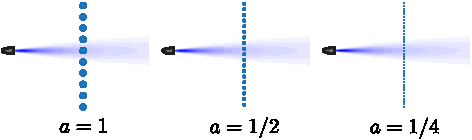
\includegraphics{decreasea.pdf}
\caption{An illustration of the continuum limit: measuring the observable $\phi^{(a)}( f_x)$. Here the quantum lattice is illustrated for several different values of the lattice spacing $a$. As $a$ gets smaller any fixed measurement of the quantum spin centred on $x$ will necessarily address more and more spins. The continuum limit is given by a limiting value $\phi(f_x)$}
\end{figure}
\paragraph{The classical continuum limit}\hspace{-1em}.---The key to understanding how to take a continuum limit is to work out an operationally meaningful way to compare states $\rho_a$ and $\rho_{a'}$ associated with \emph{different} lattice spacings $a\not=a'$. Naively this is impossible unless $a=a'$ because the quantum spins typically live at different locations. The core idea is to compare states by agreeing on a family of \emph{observables} $\{O_a\}_{a\in\mathbb{R}^+}$, indexed by $a$, which are understood to refer to the \emph{same} experiment, only discretised on a lattice with spacing $a$. If $\rho_a(O_a) \approx \rho_{a'}(O_{a'})$ for all observables $O_a$ then we declare the two states to be close. A physical justification for this notion is as follows. Imagine we have a quantum spin chain and we perform a neutron scattering experiment to measure, for example, the $z$-component of a spin at physical position $x$. The impinging beam of neutrons, even if well collimated, will inevitably spread as it travels toward the spin chain \footnote{Admittedly this analogy is a little stretched; real neutron scattering experiments cannot usually address single spins.}. Thus the observable measured by this scattering experiment is, instead of $\sigma^z_{\lfloor x/a \rfloor}$, rather $\phi^{(a)}(f_x) \equiv a\sum_{j\in\mathbb{Z}} f_x(aj) \sigma_j^z$, where $f_x$ is the \emph{beam shape} (for example, a gaussian centred at $x$: $f_x(y) \approx e^{-(y-x)^2}$). Thus the beam addresses approximately $1/a$ spins. Even though the lattice spacing $a$ of the quantum lattice system isn't precisely known, we declare that $\phi^{(a)}(f_x)$ corresponds the same experimental setup, i.e., the ``measurement of the spin at location $x$''. 

Motivated by this example we declare the family of observables given by
\begin{equation}
	\phi^{(a)}(f) \equiv a\sum_{j\in\mathbb{Z}} \sum_{\alpha=0}^{d^2-1} [f]_\alpha(aj) \lambda_j^\alpha,
\end{equation}
where $f$ is a $d^2$-dimensional vector-valued function \footnote{Suppose that $v$ is a $d$ dimensional vector. We exploit the notation $[v]_\alpha$, $\alpha=0,1,\ldots, d-1$ for the components of the vector.}, and all products and linear combinations thereof, to be the correct method to compare states on quantum lattices with different lattice spacings. That is, we say $\rho_a$ and $\rho_{a'}$ are close if $\tr(\rho_a \phi^{(a)}(f_1)\cdots \phi^{(a)}(f_m)) \approx \tr(\rho_{a'} \phi^{(a')}(f_1)\cdots \phi^{(a')}(f_m))$ for all possible choices of local rapidly decaying continuous vector-valued functions $f_l$, $l= 1, 2, \ldots, m$, with components $[f_l]_{\alpha}(x)$, for $\alpha = 0, 1, \ldots d^2-1$. {\color{red} Note open issue \#1 in the github issue queue: observables in $O_a$ given as smeared-out single-site observables are legitimate enough observables, however, \emph{products} of them are not necessarily hermitian. What is desirable here is a nice locally defined CP map which would yield a reasonable definition for multi-spin observables at scale $a$.}

The terminology ``classical continuum limit'' is justified upon noting the important fact that the operators $\phi^{(a)}(f)$ commute with each other in the limit $a\rightarrow 0$: $\lim_{a\rightarrow 0}\|[\phi^{(a)}(f), \phi^{(a)}(g)]\| =  0$. Thus, in the limit $a\rightarrow 0$, the observables $\phi^{(a)}(f)$ may be jointly measured; the set of limiting observables forms a commutative algebra and therefore models an effective classical system \footnote{If, instead, we worked with a lattice of fermions instead of quantum spins we would see that the operators $\phi_{A}^{(a)}(f)$ \emph{anticommute} with each other in the limit $a\rightarrow 0$, i.e., they give a representation of the grassmann numbers.}.

The classical continuum limit is then \emph{defined} by the expectation values of $\phi^{(a)}(f)$ for $a\rightarrow 0$, as $f$ runs over all possible ``beam shapes'':
\begin{equation}
	\left\langle\prod_{l=1}^m\phi(f_l)\right\rangle \equiv \lim_{a\rightarrow 0} \tr\left(\rho_a \prod_{l=1}^m\phi^{(a)}(f_l)\right),
\end{equation}
provided this limit exists. We say that $\{\rho_a\}_{a\in\mathbb{R}^+}$ \emph{admits a classical continuum limit} if these expectation values are finite for all rapidly decaying vector-valued functions $f_l$ \footnote{By ``rapidly decaying function'' we mean \emph{tempered distribution}.}. Note the relation $\phi(f+g) = \phi(f) + \phi(g)$.

It is worth pausing to explore a couple of simple examples to get a feeling for the classical continuum limit construction. Consider the case where $\mathcal{A} = M_2(\mathbb{C})$, i.e., our system is a chain of qubits, and $\rho_a = \bigotimes_{j\in\mathbb{Z}} \varrho$, where $\varrho$ is some single-qubit state. That is, $\rho_a$ is a mean-field ansatz independent of lattice spacing. In this case it is relatively easy to show that $\left\langle\prod_{l=1}^m\phi(f_l)\right\rangle = \prod_{l=1}^m\left\langle\phi(f_l)\right\rangle$ and $\left\langle\phi(f)\right\rangle = \sum_{\alpha=0}^3\tr(\lambda^\alpha\varrho) \int [f]_\alpha(x) \, dx$.

The second example is hardly different from the first, except that we now set $\rho_a = \bigotimes_{j\in\mathbb{Z}} \varrho(ja)$, with $\varrho(x) \equiv \frac{1}{2}\sum_{\alpha=0}^3r_{\alpha}(x)\sigma^\alpha$, where $r_\alpha(x) = (1, r_1(x), r_2(x), r_3(x))$  is some continuous vector-valued function of $x\in \mathbb{R}$ and $\sigma^0 \equiv \mathbb{I}$, $\sigma^1 \equiv \left(\begin{smallmatrix}0 & 1\\ 1 & 0\end{smallmatrix}\right)$, $\sigma^2 \equiv  \left(\begin{smallmatrix}0 & -i\\ i & 0\end{smallmatrix}\right)$, and  $\sigma^3 \equiv \left(\begin{smallmatrix}1 & 0\\0 & -1\end{smallmatrix}\right)$. In this case we again find that $\left\langle\prod_{l=1}^m\phi(f_l)\right\rangle = \prod_{l=1}^m\left\langle\phi(f_l)\right\rangle$. However, we now have that $\left\langle\phi(f)\right\rangle =  \sum_{\alpha=0}^3\int [f]_\alpha(x) r_\alpha(x) \, dx$.

We now implicitly define the (vector) \emph{field operator} $\phi(x)$ to be that object which gives $\phi(f)$ according to the relation 
\begin{equation}
	\phi(f) = \sum_{\alpha=0}^{d^2-1}\int f_\alpha(x) [\phi]_\alpha(x)\,dx, 
\end{equation}
for all $f$. For the first example above we find that  $\phi(x)$ takes a constant definite value: $[\phi]_\alpha(x) = \tr(\sigma^\alpha \varrho)$. In the second example the field takes a nonconstant definite value: $[\phi]_\alpha(x) = r_\alpha(x)$, with $r_0(x) = 1$.  In both cases the observable $\phi(x)$ takes some definite value.

However, the field operator $\phi(x)$ is not a simple function. We emphasise that $\phi(x)$ is, rather, a classical \emph{observable} and, in the case where $\rho_a$  yields a statistical ensemble in the classical continuum limit --- an example is $\rho_a = \frac12 \rho_a' + \frac12 \rho_a''$, with $\rho_a'$ and $\rho_a''$ taking different classical continuum limits --- we see that $\phi(x)$ doesn't always take a definite value. 

\paragraph{Fluctuations: the quantum continuum limit}\hspace{-1em}.---The classical continuum limit construction is essentially a law of large numbers result: the operators $\phi^{(a)}$ are the (weighted) arithmetic mean of roughly $1/a$ independent observables so that if the sequence $\{\rho_a\}_{a\in\mathbb{R}^+}$ is sufficiently well behaved we are guaranteed the existence of the limit. To see any quantum structure in the continuum we need to analyse and model the \emph{fluctuations} around the mean value of the observables $\phi^{(a)}(f)$ as the lattice spacing is decreased. Such fluctuations are detected by observables of the form
\begin{equation}
	\widetilde{\phi}^{(a)}(f) \equiv Z_f(a)\left( a\sum_{\alpha=0}^{d^2-1}\sum_{j\in \mathbb{Z}} [f]_\alpha(aj) \lambda^\alpha_j - \langle\phi(f)\rangle\mathbb{I}\right),
\end{equation}
where $Z_f(a)$ is a \emph{renormalisation} chosen to amplify the fluctuations. Central limit theorem considerations strongly suggests that these fluctuations will typically be on the order of $\sqrt{a}$; so we tentatively choose $Z_f(a) = 1/\sqrt{a}$ in order to ensure the fluctuations remain present in the limit $a\rightarrow 0$. From the perspective of a scattering experiment interpretation what we are doing is increasing the sensitivity of our detection apparatus to amplify the fluctuations due to microscopic features: if the experimentalist leaves the sensitivity of the detector constant then this experiment will only be sensitive to the bulk classical fields $\phi(x)$ and the experimentalist is content with a classical model for the statistical fluctuations in $\phi(x)$ due to the ensemble of classical limits. If, however, the experimentalist improves the detector to be sensitive to fluctuations of the order of $\sqrt{a}$ then, on top of the original statistical fluctuations, \emph{additional} fluctuations will emerge, now with a possibly quantum explanation. We now make this precise. 

Analogous to the classical case, the quantum continuum limit is defined by the expectation values of $\widetilde{\phi}^{(a)}(f)$ for $a\rightarrow 0$, as $f$ runs over all rapidly decaying vector-valued functions:
\begin{equation}\label{eq:qctslimit}
	\langle\Omega|\left(\prod_{l=1}^m\widehat{\phi}(f_l)\right)|\Omega\rangle \equiv \lim_{a\rightarrow 0} \tr\left(\rho_a \prod_{l=1}^m\widetilde{\phi}^{(a)}(f_l)\right),
\end{equation}
provided this limit exists \footnote{Here the order of the products matters; we henceforth take all product symbols as running from left to right: $\prod_{l=1}^m M_l \equiv M_1M_2\cdots M_m$.}. Thus $\{\rho_a\}_{a\in\mathbb{R}^+}$ is said to admit a \emph{quantum continuum limit} if these expectation values are finite for all rapidly decaying functions $f_l$. It is sometimes necessary in the sequel to relax this requirement and only demand that a subset of the limits exist, typically for operators admitting an interpretation as canonical field amplitude observables (in such a case we obtain a \emph{singular} state, in the sense of operator algebras). This innocuous-seeming condition is deeply nontrivial; one of the main contributions of this paper is to show that there are families of tensor network states for which this condition is fulfilled. 

The expectation value in Eq.~(\ref{eq:qctslimit}) is taken with respect to a \emph{pure state} $|\Omega\rangle$; we now show how this state is constructed and justify the notation $\langle\Omega|\cdot |\Omega\rangle$ for the limiting functional. Because $\lim_{a\rightarrow0} \tr(\rho_a) = 1$ we have that the limiting functional is normalised: $\langle\Omega| \mathbb{I} |\Omega\rangle = 1$. Secondly, we inherit linearity in the limit: $\langle \Omega| (\alpha \widehat{\phi}(f) + \beta\widehat{\phi}(g))|\Omega\rangle = \lim_{a\rightarrow 0} \tr\left(\rho_a \left(\alpha \widetilde{\phi}^{(a)}(f) + \beta \widetilde{\phi}^{(a)}(g)\right) \right)$ $= \alpha\lim_{a\rightarrow 0} \tr\left(\rho_a  \widetilde{\phi}^{(a)}(f)\right)$ + $\beta\lim_{a\rightarrow 0} \tr\left(\rho_a \widetilde{\phi}^{(a)}(g)) \right)$ $=  \alpha \langle \Omega| \widehat{\phi}(f) |\Omega\rangle+ \beta\langle \Omega|\widehat{\phi}(g)|\Omega\rangle$. Finally we have that the limiting functional is positive: $\langle\Omega | \widehat{\phi}(f)^\dag \widehat{\phi}(f) |\Omega\rangle$ $= \lim_{a\rightarrow 0} \tr(\rho_a (\widetilde{\phi}^{(a)}(f)^\dag \widetilde{\phi}^{(a)}(f))) \ge 0$. (These arguments remain true for products of the fluctuation operators.) Thus the limiting object is a state. Further, we can always purify the limiting state to $|\Omega\rangle$, justifying the notation $\langle \Omega|\cdot|\Omega\rangle$.

Using the state $|\Omega\rangle$ we now describe the hilbert space $\mathcal{H}$ of quantum field fluctuations: this is simply the hilbert space built from $|\Omega\rangle$ and all vectors of the form $\left(\prod_{l=1}^m\widehat{\phi}(f_l)\right)|\Omega\rangle$. (It is a nontrivial fact that this construction leads to a separable hilbert space.) In terms of these vectors a fluctuation operator $\widehat{\phi}(f)$ acts as
\begin{equation}	
	\widehat{\phi}(f) \left(\prod_{l=1}^m\widehat{\phi}(f_l)\right)|\Omega\rangle \equiv \widehat{\phi}(f) \widehat{\phi}(f_1)\cdots \widehat{\phi}(f_m)|\Omega\rangle.
\end{equation}

A remarkable consequence --- similar to the original quantum fluctuation construction \cite{hepp:1973b, verbeure:2011a} --- of the fluctuation field construction is that the limiting objects obey the bosonic canonical commutation relations: as long as $Z_f(a)Z_g(a) = 1/a$ we have that $[\widehat{\phi}(f), \widehat{\phi}(g)] = \langle \phi(f\wedge g)\rangle \mathbb{I}$ \footnote{The wedge product between two vector-valued functions $f$ and $g$ is defined as follows. First write $\lambda^\alpha\lambda^\beta =  \frac12{d^{\alpha\beta}}_\gamma \lambda^\gamma + \frac{i}{2}{f^{\alpha\beta}}_{\gamma}\lambda^\gamma$ for the structure constants of the operator basis $\lambda^\alpha$, where ${d^{\alpha\beta}}_\gamma$ (respectively, ${f^{\alpha\beta}}_{\gamma}$) are the completely symmetric (respectively, antisymmetric) structure constants. The wedge product of two vectors $u$ and $v$  is then defined to be the vector with components $[u\wedge v]_{\gamma} = \sum_{\alpha,\beta=0}^{d^2 -1}[u]_\alpha[v]_\beta {f^{\alpha\beta}}_\gamma$. Thus the wedge product $f\wedge g$ of two vector-valued functions is the vector-valued function $f(x)\wedge g(x)$.}. This surprising fact is proved as follows.  Consider
\begin{equation}
	\begin{split}
		[\widetilde{\phi}^{(a)}(f), \widetilde{\phi}^{(a)}(g)] &= a^2Z_f(a)Z_g(a)\sum_{j\in\mathbb{Z}} [f\wedge g]_\gamma(aj) \lambda^\gamma_j \\
		&= \phi^{(a)}(f\wedge g).
	\end{split}
\end{equation} 
this expression may be rewritten as a local fluctuation operator:
\begin{equation}
	[\widetilde{\phi}^{(a)}(f), \widetilde{\phi}^{(a)}(g)] = \langle\phi(f\wedge g)\rangle \mathbb{I} + Z_{f\wedge g}^{-1}(a)\widetilde{\phi}^{(a)}(f\wedge g).
\end{equation}
Assuming that ${Z_{f\wedge g}^{-1}(a)} \underset{a\rightarrow 0}{\rightarrow} 0$ we have that $[\widetilde{\phi}^{(a)}(f), \widetilde{\phi}^{(a)}(g)]$ is given by a constant term plus an operator decaying to $0$ on the hilbert space of fluctuations. Thus, in any expectation value, we can replace any commutator $[\widehat{\phi}(f), \widehat{\phi}(g)]$ with the number $\langle \phi(f\wedge g)\rangle \mathbb{I}$, i.e., 
\begin{equation}\label{eq:ccr}
	[\widehat{\phi}(f), \widehat{\phi}(g)] = \langle \phi(f\wedge g)\rangle \mathbb{I}.
\end{equation}
We now identify this algebraic structure with the canonical commutation relations. 

To understand the algebraic properties of the operators $\widehat{\phi}(f)$ it is convenient (but not necessary) to specialise to the translation invariant case. Here we have that 
\begin{equation}
	\langle \phi(f\wedge g)\rangle = \lim_{a\rightarrow 0} \tr(\rho_a [\lambda^\alpha,\lambda^\beta]) ([\overline{f}]_\alpha,[g]_\beta), 
\end{equation}
where $(f,g) = \int \overline{f}(x)g(x)\,dx$.
 Form the hermitian antisymmetric matrix $\Theta$ with matrix elements $[\Theta]_{\alpha\beta}  \equiv \lim_{a\rightarrow 0} \tr(\rho_a [\lambda^\alpha,\lambda^\beta])$. The matrix $\Theta$ induces an antisymmetric form $\Theta(A,B) \equiv \sum_{\alpha,\beta} a_\alpha b_\beta [\Theta]_{\alpha\beta}$ for $A = \sum_{\alpha=0}^{d^2-1} a_\alpha \lambda^\alpha$ and  $B = \sum_{\alpha=0}^{d^2-1} b_\beta \lambda^\beta$. Applying the symplectic Gram-Schmidt procedure (see Appendix) to this symplectic form produces a list of three hermitian operators $\{\mu^{j}, \nu^{j}\}_{j=1}^m$ and  $\{\xi^{j}\}_{j = 1}^{D^2-2m}$ such that $\Theta(\mu^j, \nu^k) = i\delta^{jk}$ and $\Theta(\xi^j, M) = 0$ for any $M$ which is a linear combination of $\mu^j$ and $\nu^j$. Let $f$ be a function with rapid decay and define $[a_j]_\alpha(x) \equiv f(x) \tr(\lambda^\alpha\mu^j)$, $[b_j]_\alpha(x) \equiv f(x) \tr(\lambda^\alpha\nu^j)$, and $[c_j]_\alpha(x) \equiv f(x) \tr(\lambda^\alpha\xi^j)$ We then define $\widehat{\varphi}_j(f) \equiv \widehat{\phi}(a_j)$ and $\widehat{\pi}_j(f) \equiv \widehat{\phi}(b_j)$, and $\widehat{\xi}_j(f) \equiv \widehat{\phi}(c_j)$. According to Eq.~(\ref{eq:ccr}) we then have that
\begin{equation}
	[\widehat{\varphi}_j(f), \widehat{\pi}_k(g)] = i (\overline{f},g)\delta^{jk} \mathbb{I}.
\end{equation}
Both of the operators $\widehat{\varphi}_j$ and $\widehat{\pi}_j$ are hermitian.
Finally, we implicitly define the quantum field operator $\widehat{\varphi}_j(x)$ via
\begin{equation}
	\widehat{\varphi}_j(f) \equiv \int f(x)\widehat{\varphi}_j(x)\,dx,
\end{equation}
and similarly for $\widehat{\pi}_j(x)$. In the case where the original lattice system was fermionic we obtain the canonical anticommutation relations instead.

Let's now apply the quantum continuum limit construction to some examples. The first is the product-state example $\rho_a = \bigotimes_{j\in\mathbb{Z}}\varrho$. We first construct the matrix $\Theta(\sigma^\alpha,\sigma^\beta) \equiv \frac12\sum_{\gamma=0}^3 r_\gamma \tr([\sigma^\alpha,\sigma^\beta]\sigma^\gamma)$. We assume, for simplicity, that $r = (0,0,0,1)$. (The general case is discussed in the Appendix.) In this case we find that $\mu^0 = \mathbb{I}$, $\mu^1 = \sigma^z$, $\nu^1 = \sigma^x$, and $\xi^1 = \sigma^y$. We thus recover standard fock space with vacuum state $|\Omega\rangle$.

The second example we study is that of a sequence of matrix product states $|\psi_a\rangle = \sum\langle \omega_L| \cdots A^{z_{-1}}_aA^{z_{0}}_a A^{z_{1}}_a\cdots |\omega_R\rangle |\cdots z_{-1}z_0z_{1} \cdots \rangle$
with the prescription $A^0_a \equiv \mathbb{I} + a Q$ and $A^1_a \equiv \sqrt{a} R$, where $Q$ and $R$ are $D\times D$ complex matrices. In this case we again find that the classical limit is a trivial product. The theta matrix is identical to the product state case, and we obtain the same quantum fluctuation operators. Thus the quantum field modelling the fluctuations around an MPS is precisely that of a single bosonic degree of freedom. However, in contrast to the product state case, the continuum limit state $|\Omega\rangle$ is \emph{not} the fock vacuum and nor is it generically gaussian. Indeed, it is precisely a continuous matrix product state $|\Omega\rangle \equiv \langle\omega_L|\mathcal{P}e^{\int_{-\infty}^\infty Q\otimes\mathbb{I} + R\otimes \widehat{\psi}^\dag(s)\,ds}|0\rangle|\omega_R\rangle$,  where $|0\rangle$ is the fock vacuum. 

\paragraph{Dynamics of quantum fluctuations}\hspace{-1em}.---Suppose we have a sequence $\rho_a$ giving rise to a quantum continuum limit and suppose, further, that we have a sequence  of hamiltonians $H_a\ge 0$ such that $\tr(H_a\rho_a) = 0$, $\forall a$. We can study the dynamics $U_a(t) = e^{itH_a}$ this sequence of hamiltonians generates for fluctuations around the continuum limit as follows. If $H_a$ is a sequence of nearest-neighbour hamiltonians for a quantum spin system then simple dimensional analysis leads requires that we must scale time via $t\mapsto t/a$. Thus we study the dynamics generated by the unitary $U_a(t/a)$ in the continuum limit. It is natural to expect that there is a continuum hamiltonian $\widehat{H}$ which generates the limiting dynamics. A useful mnemonic to derive this hamiltonian is that we can identify $\lambda^{\alpha}_{j} \equiv {Z_{\lambda^\alpha}^{-1}}\widetilde{\phi}^{(a)}(\delta_{\alpha\beta}\delta(ja))$. 

Rather astonishingly it turns out that the dynamics generated by $\widehat{H}$ obeys strict causality: there is an \emph{exact} lightcone for the propagation of information through the continuous system. This is a consequence of the Lieb-Robinson bound  \cite{lieb:1972a,bratteli:1997a,nachtergaele:2010b}: we have that there is a universal constant $c$ for all $A$ and $B$ such that
\begin{equation}
	[\widehat{\phi}(f), e^{-it\widehat{H}} \widehat{\phi}(g)e^{it\widehat{H}} ] = 0
\end{equation}
whenever $\dist(\supp(f) , \supp(g)) < ct$. However, we don't generally obtain Poincar\'e invariance of the quantum continuum limit unless the excitation structure of $H$ exhibits more structure (rotation invariance is typically broken in most lattice models --- an effect that persists in the continuum limit.) 

As a simple application of this prescription we study the continuum limit of the product states $\rho_a = \bigotimes |0\rangle\langle 0|$ with corresponding hamiltonian given by the ferromagnetic $XY$ model, i.e., $H_a = \frac{1}{a}\sum_{j} \mathbb{I} - \sigma^x_j\sigma_{j+1}^x - \sigma^y_j\sigma_{j+1}^y$. Following the identification $\sigma^x_j \equiv \sqrt{a}\widetilde{\varphi}^{(a)}(\delta(ja))$, $\sigma^y_j \equiv \sqrt{a}\widetilde{\pi}^{(a)}(\delta(ja))$, and $\sigma^z_j \equiv \sqrt{a}\widetilde{\xi}^{(a)}(\delta(ja))$ we find
\begin{equation}
	\widehat{H} = \int \widehat{\varphi}(x) \partial_x\widehat{\varphi}(x) + \widehat{\pi}(x) \partial_x\widehat{\pi}(x) \, dx.
\end{equation}
We thus recover the result that, in the heisenberg picture, the fluctuation field obeys the wave equation:
\begin{equation}
	\partial_{tt}\widehat{\varphi}(x,t) = \partial_{xx}\widehat{\varphi}(x,t).
\end{equation}
Solutions to this equation obey strict causality, in accordance with the argument above.

\paragraph{Strings: extending the observable algebra}\hspace{-1em}.---As is now well understood, especially in higher dimensions, there is the possibility for quantum systems to exhibit stringlike excitations in different superselection sectors This naturally occurs in a symmetry broken phase where kinklike solutions interpolating between different ground states are possible particles. In many cases we have a characterisation of the corresponding string operators, for example for matrix product states \cite{perez-garcia:2008a}, and we can extend the continuum limit construction to incorporate these observables \footnote{This limitation can also be lifted by employing the ``wedge algebra'' construction: fix a cone $\Lambda$ in the lattice system and construct, for each $a$, the \emph{bicommutant} $\mathcal{M}_a(\Lambda) \equiv \mathcal{A}_a(\lambda)''$ of the algebra of all discretised field operators whose support functions $f$ lie totally within the cone $\Lambda$.  This gives, in the limit $a\rightarrow 0$, a von Neumann algebra of observables on the cone $\Lambda$.}. In this case we observe a transmutation of statistics where fermionic and anyonic excitations can emerge. 

\paragraph*{Conclusions}\hspace{-1em}.---We have introduced a procedure, based on the \emph{fluctuation construction} of Hepp and Lieb, Verbeure and coworkers, which takes a sequence of states of a quantum lattice system and produces a corresponding list of quantum field data for the limiting state. This method was applied to several natural tensor network classes yielding their well-known (and not so well-known) continuous analogues. In combination with the tensor network sequence developed in the companion paper to this one we are able to obtain nontrivial states of continuous quantum Yang-Mills theory.

\acknowledgments{This work was supported by the ERC grants QFTCMPS and SIQS, and by the cluster of excellence EXC 201 Quantum Engineering and Space-Time Research.}

\bibliography{clqls}

\widetext
\appendix
\section{$\star$-vector spaces and the Gram-Schmidt procedure}\label{app:ags}
In this appendix we review the elements of $\star$-vector spaces, skew-symmetric maps, and the Gram-Schmidt procedure.

\begin{definition}
	A \emph{$\star$-vector space} consists of a complex vector space $V$ and an involutive conjugate linear map $\star:V\rightarrow V$, i.e., $(\lambda v + w)^\star = \overline{\lambda}v^\star + w^\star$ for all $\lambda \in \mathbb{C}$ and $v,w \in V$. If $V$ is a $\star$-vector space then we denote by $V_h$ the \emph{hemitian elements} of $V$, which is the set given by
	\begin{equation}
		V_h \equiv \{x\in V\,|\, x^\star = x\}.
	\end{equation}
\end{definition}

The subspace $V_h$ is a real subspace of the complex vector space $V$. There is always a decomposition of any $v\in V$ via
\begin{equation}
	v = x+iy, 
\end{equation}
where $x,y \in V_h$ are given by 
\begin{equation}
	x = \frac{v+v^\star}{2},\quad\text{and}\quad y = \frac{v-v^\star}{2i}.
\end{equation} 
The vectors $x$ and $y$ are called the \emph{real} and \emph{imaginary} parts of $v$. Thus we have the decomposition
\begin{equation}
	V \cong V_h\oplus iV_h,
\end{equation}
as real vector spaces.

Suppose we have a sesquilinear inner product $(\cdot ,\cdot )$ on $V$. In terms of the real and imaginery parts we have
\begin{equation}
	(v,w) = (x+iy, x'+iy') = (x,x') - i(y,x') + i(x,y') + (y,y'),
\end{equation}
i.e., the inner product is determined by its values on $V_h$.

\begin{example}
	Let $\mathcal{H}$ be a finite-dimensional hilbert space and $V \equiv \mathcal{B}(\mathcal{H})$ the set of bounded operators on $\mathcal{H}$. The vector space $V$ is naturally a $\star$-vector space according to the involution given by the hermitian conjugate operation $A\mapsto A^\dag$. It is easy to check that $V_h$ is exactly the space of hermitian operators. The space 
	
	Let $\rho$ be a density operator on $\mathcal{H}$ and endow $V$ with the inner product 
	\begin{equation}
		\langle A, B\rangle \equiv \tr(\rho A^\dag B).
	\end{equation}
	We consider the alternating form $\Omega$ on $V_h$ given by
	\begin{equation}
		\Omega(A,B) \equiv \tr(\rho [A,B]) = \langle A, B\rangle-\langle B, A\rangle.
	\end{equation}
	This may be extended to $V \cong V_h\oplus iV_h$ by defining
	\begin{equation}
		\Omega(iA,iB) \equiv -\Omega(A,B),
	\end{equation}
	and
	\begin{equation}
		\Omega(A,iB) \equiv i\Omega(A,B) = \Omega(iA,B)
	\end{equation}
	for all $A,B\in V_h$ and extending by linearity.
\end{example}


Let $V$ be an $m$-dimensional real vector space and let $\Omega:V\times V \rightarrow \mathbb{R}$ be a skew form, i.e., a bilinear map such that
\begin{equation}
	\Omega(u, v) = -{\Omega(v,u)},
\end{equation}
for all $u, v\in V$.
\begin{theorem}[Standard form]
	Let $\Omega$ be a skew-symmetric bilinear form on $V$. Then there is a basis $u_1, \ldots, u_k$, $e_1, \ldots, e_n$, $f_1, \ldots, f_n$ of $V$ such that
	\begin{equation}
		\begin{split}
			\Omega(u_j, v) = 0, \quad &\text{for all $j$ and $v\in V$}, \\
			\Omega(e_j, e_k) = 0 = \Omega(f_j, f_k), \quad &\text{for all $j$ and $k$, and}, \\
			\Omega(e_j, f_k) = \delta_{jk},\quad &\text{for all $j$ and $k$.} \\
		\end{split}
	\end{equation}
\end{theorem}
\begin{proof}
	Let $U \equiv \{u\in V\,|\, \Omega(u,v) = 0, \forall v\in V\}$. Choose a basis $u_1, \ldots, u_k$ of $U$, and choose a complementary space $W$ to $U$ in $V$, i.e., 
	\begin{equation}
		V = U\oplus W.
	\end{equation}
		
	Take a nonzero $e_1\in W$. Then there is an $f_1\in W$ such that $\Omega(e_1, f_1) \not= 0$. Rescale $e_1$ and $f_1$ so that $\Omega(e_1,f_1) = 1$. Let 
	\begin{equation}
		\begin{split}
			W_1 &= \langle e_1, f_1 \rangle, \quad \text{and} \\
			W_1^{\Omega} &= \{w\in W\,|\, \Omega(w, v) = 0, \forall v\in W_1\}.
		\end{split}
	\end{equation}

We now argue that $W_1\cap W_1^{\Omega}= \{0\}$. Suppose that $v = ae_1 + bf_1 \in W_1\cap W_1^{\Omega}$. Then we have that
\begin{equation}
	0 = \Omega(v,e_1) = -b, \quad \text{and} \quad 0 = \Omega(v, f_1) = a.
\end{equation}
But this means that $v=0$.

Next we argue that $W = W_1\oplus W_1^{\Omega}$. Suppose that $v\in W$ has $\Omega(v, e_1) = c$ and $\Omega(v, f_1)= d$. Then
\begin{equation}
	v = v_{\|} + v_{\perp},
\end{equation}
with $v_{\|} = -cf_1 + d e_1 \in W_1$ and $v_{\perp} = v+cf_1-de_1 \in W_1^\Omega$.

Repeat this process by choosing $e_j\in W_j^\Omega$, $e_j\not=0$. Then there is $f_j$ such that $\Omega(e_j,f_j) = 1$. Let $W_j$ be span of $e_j$ and $f_j$.

Because $V$ is assumed finite dimensional this process terminates and we obtain
\begin{equation}
	V = U\oplus W_1\oplus W_2 \oplus \cdots \oplus W_n.
\end{equation}
\end{proof}

\section{The spacetime continuum limit}
So far the continuum limit construction has been limited to the discussion of \emph{kinematics}, i.e., we only discuss the hilbert-space structure for the continuous limit. In this appendix we extend the continuum limit construction to accommodate dynamics. 

The natural setting here is then that of a quantum lattice system in $D$ dimensions with hamiltonian 
\begin{equation}
	H_a \equiv \sum_{\langle j,k\rangle } h_{j,k}(a),
\end{equation}
where the sum is over all neighbouring spins. We allow the hamiltonian to possibly depend on the lattice spacing $a$, however, the norm $\|h_{j,k}(a)\|$ is required to be bounded by a constant for all sites $j$ and $k$ in the lattice. 

As we'll see later, such an identification leads to a definition of the dynamics for the continuum limit which obeys strict causality. This argument is essentially conditioned on the existence of a \emph{spacetime} quantum continuum limit which is defined in the following. First introduce the classical \emph{spacetime} discretised field operators via
\begin{equation}
	\phi^{(a)}(f) \equiv a^{D+1}\sum_{\alpha = 0}^{d^2-1}\sum_{j\in\mathbb{Z}^D} \int_{-\infty}^\infty f_\alpha(at, aj) e^{-itH_a}\lambda^\alpha_je^{itH_a} \, dt,
\end{equation}
where now $f$ is a rapidly decaying function on spacetime $\mathcal{M}_{D+1}\equiv\mathbb{R}\times \mathbb{R}^D$. We say that the sequence 
$\{\rho_a\}_{a\in\mathbb{R}^+}$ admits a \emph{classical spacetime continuum limit} if 
\begin{equation}
	\left\langle\prod_{l=1}^m\phi(f_l)\right\rangle \equiv \lim_{a\rightarrow 0} \tr\left(\rho_a \prod_{j=l}^m\phi^{(a)}(f_l)\right)
\end{equation}
for all rapidly decaying $f_l$ on $\mathcal{M}_{D+1}$.

We define the spacetime quantum fluctuation operators via
\begin{equation}
	\widetilde{\phi}^{(a)}(f) \equiv Z_f(a)\left( \int_{-\infty}^\infty  a^{D+1}\sum_{\alpha = 0}^{d^2-1}\sum_{j\in \mathbb{Z}^D} f_\alpha(at, aj) e^{-itH_a}\lambda^\alpha_je^{itH_a} \,dt - \langle\phi(f)\rangle\mathbb{I}\right).
\end{equation}
Correspondingly, the \emph{quantum spacetime continuum limit} is defined by the expectation values of products of $\widetilde{\phi}^{(a)}(f)$ for $a\rightarrow 0$, as $f$ runs over all rapidly decaying functions on $\mathcal{M}_{D+1}$:
\begin{equation}\label{eq:qsctslimit}
	\langle\Omega|\left(\prod_{l=1}^m\widehat{\phi}(f_l)\right)|\Omega\rangle \equiv \lim_{a\rightarrow 0} \tr\left(\rho_a \prod_{l=1}^m\widetilde{\phi}^{(a)}(f_l)\right),
\end{equation}
provided this limit exists.
(At this point it is worth noting that we can also obtain continuum limits for dynamics generated by discrete groups, e.g., quantum cellular automata, by replacing the integral over $t$ with a sum.)



%\section{The GNS construction}
%In this appendix we collect some basic results concerning $*$-algebras and representations. The presentation here can be found in many standard texts, e.g., \cite{dixmier:1977a} and \cite{kadison:1997a}. In contrast to usual presentations we quote our results for $*$-algebras rather than $C^*$-algebras.
%\begin{definition}
%	An associative algebra $\mathcal{A}$ over $\mathbb{C}$ is called a $*$-algebra if it is equipped with a map $A\mapsto A^*$ which is anti-linear, involutive, and an anti-automorphism. 
%\end{definition}
%
%\begin{definition}
%	Let $\mathcal{A}$ be a $*$-algebra over $\mathbb{C}$. A linear functional $\omega:\mathcal{A}\rightarrow \mathbb{C}$ is called \emph{positive} if
%	\begin{equation}
%		\omega(A^*A) \ge 0, \quad \forall A\in\mathcal{A}.
%	\end{equation}
%If $\mathcal{A}$ is \emph{unital} (i.e., it has an identity element $\mathbb{I}$) we say that $\omega$ is a \emph{state} if $\omega(\mathbb{I}) = 1$. An element $A\in\mathcal{A}$ is \emph{algebraically positive} if we can write
%\begin{equation}
%	A = \sum_{j=1}^n b_j B^*_jB_j,
%\end{equation}
%with $b_j>0$ and $B_j\in \mathcal{A}$. An element $A \in \mathcal{A}$ is called positive if for all positive functionals $\omega:\mathcal{A}\rightarrow \mathbb{C}$ we have that $\omega(A)\ge 0$.
%\end{definition}
%The algebraically positive elements $\mathcal{A}^{++}$ are a subset of the positive elements $\mathcal{A}^+$, and both subsets are convex cones in $\mathcal{A}$. We have the \emph{Cauchy-Schwarz} inequality
%\begin{equation}
%	\omega(A^*B)\overline{\omega(A^*B)} \le \omega(A^*A)\omega(B^*B),
%\end{equation}
%for all $A,B\in \mathcal{A}$.
%
%\begin{definition}
%	Let $\mathcal{A}$ be a $*$-algebra over $\mathbb{C}$. A $*$-representation $\pi$ of $\mathcal{A}$ on a hilbert space $\mathcal{H}$ is a $*$-homomorphism $\pi:\mathcal{A}\rightarrow \mathcal{B}(\mathcal{H})$.
%\end{definition}
%
%\begin{definition}
%	Let $\omega:\mathcal{A}\rightarrow \mathbb{C}$ be a positive linear functional and define
%	\begin{equation}
%		\mathcal{J}_\omega = \{A\in \mathcal{A}\,|\, \omega(A^*A) = 0\}.
%	\end{equation}
%\end{definition}
%The Cauchy-Schwarz inequality shows that $\mathcal{J}_\omega$ is a left ideal, called the \emph{Gel'fand ideal of $\omega$}. The quotient
%\begin{equation}
%	\mathcal{H}_\omega = \mathcal{A}/\mathcal{J}_\omega
%\end{equation}
%is an $\mathcal{A}$-module with left action written $\pi_\omega(A) |B\rangle = |AB\rangle$, where $|A\rangle \in \mathcal{H}_\omega$ denotes the equivalence class of $A \in \mathcal{A}$ in the quotient. The space $\mathcal{H}_\omega$ becomes a pre-Hilbert space by
%\begin{equation}
%	\langle A|B\rangle_\omega = \omega(A^*B).
%\end{equation}
%One can verify that $\pi_\omega(A)\in \mathcal{B}(\mathcal{H}_\omega)$ and $\pi_\omega(A^*) = \pi_\omega(A)^*$, so that $\pi_\omega$ is a $*$-representation, the \emph{GNS}-representation induced by $\omega$. In the unital case one obtains a \emph{cyclic vector} $|\Omega\rangle \equiv |\mathbb{I}\rangle$, and $\pi_\omega$ is a \emph{cyclic $*$-representation} and is 
%\begin{equation}
%	\omega(A) = \langle\Omega|\pi_\omega(A)|\Omega\rangle.
%\end{equation} 

\section{Fermions}
In this appendix we generalise the continuum limit construction to the fermionic case. Our setting is again that of a regular lattice $a\mathbb{Z}^D$ embedded in $\mathbb{R}^D$, where $a>0$ is the lattice spacing. However, we now assume that, instead of a distinguishable quantum spin being attached to each site, we have a family of fermions hopping on the lattice. We describe this with a collection of operators $a_{j,\sigma}$ and $a^{\dag}_{j,\sigma}$, where $j\in a\mathbb{Z}^D$ and $\sigma \in \{1,2, \ldots, s\}$ labels some internal degrees of freedom, obeying the canonical anticommutation relations
\begin{equation}
	\{a_{j,\sigma}, a^{\dag}_{k,\tau}\} = \delta_{j,k}\delta_{\sigma\tau}.
\end{equation}

\subsection{The classical continuum limit}
We again start in one spatial dimension and employ the following natural generalisation of our classical smeared field operators for the fermionic setting
\begin{equation}
	\phi^{(a)}(f) \equiv a\sum_{j\in\mathbb{Z}} \sum_{\alpha=0}^{2^s-1} [f]_\alpha(aj) \lambda_j^\alpha,
\end{equation}
where now $f$ is a function from $a\mathbb{Z}$ to bounded operators on the space of fermions of $s$ species at a single site, i.e., $\lambda^{\alpha}_j$ runs over all suitably normalised polynomials of $a_{j,\sigma}$ and $a_{j,\sigma}^\dag$ in normal order. E.g., in the case where $s=0$,
\begin{equation}
	\lambda^0_j = \frac{1}{\sqrt{2}}\mathbb{I}_j, \quad \lambda^{1}_j = a_j, \quad \lambda^{2}_j = a_j^\dag, \quad\text{and}\quad \lambda^{3}_j = \frac{1}{\sqrt{2}}(a_j^\dag a_j - a_j a_j^\dag).
\end{equation}
The fermion algebra is $\mathbb{Z}/2\mathbb{Z}$ graded according to whether there are an even (respectively, odd) product of fermion operators.

Now it is easy to see that our classical smeared field observables also become $\mathbb{Z}/2\mathbb{Z}$ graded, according to whether they contain an even (respectively, odd) number of fermion operators. In the case of two odd smeared classical field operators we find that their commutator \emph{does not vanish} in the limit $a\rightarrow 0$. Instead, their \emph{anticommutator} vanishes according to
\begin{equation}
	\lim_{a\rightarrow 0}\|\{\phi^{(a)}(f), \phi^{(a)}(g)\}\| = 0,
\end{equation}
i.e., they become \emph{Grassmann number valued}. We define the classical limit in the fermionic case as in the bosonic case by requiring that the following limits exist
\begin{equation}
	\left\langle\prod_{l=1}^m\phi(f_l)\right\rangle \equiv \lim_{a\rightarrow 0} \tr\left(\rho_a \prod_{l=1}^m\phi^{(a)}(f_l)\right),
\end{equation}
as $f$ runs over all rapidly decaying functions. Notice that, in contrast to the bosonic case, the order of the products of the argument does, in general, matter in this expression. However, because physical states any microscopic theory must obey superselection rules, i.e., they are linear functions vanishing on odd operators, the expectation values of odd operators vanish and hence the order with respect to even operators is irrelevant.

The functional $\langle \cdot \rangle$ is a positive linear functional on the algebra of all rapidly decaying grassmann number valued functions from $\mathbb{R}$ to $\mathcal{G}_n$.

Let's study a simple example. We consider two species of fermion, spin up $a_{j,\uparrow}$ and spin down $a_{j,\downarrow}$, hopping on an infinite chain. Our reference state is given by the ground state $|\Omega\rangle$ of the simple model 
\begin{equation}
	H = \sum_{j\in\mathbb{Z}} a_{j,\uparrow}^\dag a_{j,\uparrow} - a_{j,\downarrow}^\dag a_{j,\downarrow}.
\end{equation}
This state is simply the half-filled state where there is a spin-down particle at each site:
\begin{equation}
	|\Omega\rangle \equiv \prod_{j\in\mathbb{Z}} a_{j,\downarrow}^\dag|\text{vac}\rangle,
\end{equation}
where $|\text{vac}\rangle$ is the empty vacuum state. The configuration space is $16$ dimensional and the local observable algebra has dimension $256$ and is built from the four odd operators $a_{j,\sigma}$ and $a_{j,\sigma}^\dag$, $\sigma = \uparrow, \downarrow$, and quadratic, cubic, and quartic combinations thereof.  The expectation value of the four odd field operators built from $a_{j,\sigma}$ and $a_{j,\sigma}^\dag$, $\sigma = \uparrow, \downarrow$ vanish, and hence also when they appear in any product. We are left with two nonzero classical field operators, the identity operator and the magnetisation field
\begin{equation}
	\phi(x) \equiv -1.
\end{equation}

\subsection{The quantum continuum limit}
The fermionic quantum continuous limit is derived analogously to the bosonic case: here the fermionic field fluctuation operators are by
\begin{equation}
	\widetilde{\phi}^{(a)}(f) \equiv Z_f(a)\left( a\sum_{\alpha=0}^{d^2-1}\sum_{j\in \mathbb{Z}} [f]_\alpha(aj) \lambda^\alpha_j - \langle\phi(f)\rangle\mathbb{I}\right).
\end{equation}
In contrast to the bosonic case, as we'll see, we obtain a \emph{graded} antisymmetric form for the anticommutator. 

Suppose that $Z_f(a)Z_g(a) = 1/a$ and that $f$ and $g$ are both \emph{odd} fermionic lattice operators. We now show that $\{\widehat{\phi}(f), \widehat{\phi}(g)\} \propto \mathbb{I}$. The proof of this closely follows the bosonic case.  Consider first
\begin{equation}
			\{\widetilde{\phi}^{(a)}(f), \widetilde{\phi}^{(a)}(g)\} = a^2Z_f(a)Z_g(a)\sum_{j\in\mathbb{Z}} \sum_{\alpha,\beta,\gamma=0}^{2^s-1} [f]_\alpha(aj)[g]_\beta(aj) \tr(\lambda^{\gamma}_j\{\lambda_j^\alpha, \lambda_j^\beta\})  \lambda^\gamma_j. \\
\end{equation} 
we first rewrite this expression as 
\begin{equation}
	\begin{split}
		\{\widetilde{\phi}^{(a)}(f), \widetilde{\phi}^{(a)}(g)\} &= \langle\phi(f\star g)\rangle\mathbb{I} + a\sum_{j\in\mathbb{Z}} \sum_{\alpha,\beta,\gamma=0}^{2^s-1} [f]_\alpha(aj)[g]_\beta(aj) \tr(\lambda^{\gamma}_j\{\lambda_j^\alpha, \lambda_j^\beta\})  \lambda^\gamma_j - \langle \phi(f\star g)\rangle\mathbb{I}, \\
		&= \langle\phi(f\star g)\rangle\mathbb{I} + Z^{-1}_{f\star g}(a)\widetilde{\phi}^{(a)}(f\star g),
	\end{split}
\end{equation}
where we've introduced the \emph{star product}: let $v$ and $w$ be two vectors in $\mathbb{C}^{2^s}$ and define the vector $v\star w$ via
\begin{equation}
	[v\star w]_\alpha \equiv \sum_{\beta,\gamma = 0}^{2^s-1}\tr(\lambda^{\alpha}\{\lambda^\beta, \lambda^\gamma\})[v]_\beta[w]_\gamma.
\end{equation}
The star product is extended pointwise to functions via
\begin{equation}
	(f\star g)(x) \equiv f(x)\star g(x).
\end{equation}
Thus, as long as $\lim_{a\rightarrow 0} Z^{-1}_{f\star g}(a) = 0$, we can replace, in the limit $a\rightarrow 0$, the anticommutator of $\widetilde{\phi}^{(a)}(f)$ and $\widetilde{\phi}^{(a)}(g)$ with a multiple of the identity inside any expectation value. Hence we deduce the anticommutation relations for the odd quantum field fluctuation  operators
\begin{equation}
	\{\widehat{\phi}(f), \widehat{\phi}(g)\} = \langle\phi(f\star g)\rangle\mathbb{I}.
\end{equation}

\subsection{The tight-binding model}
The simplest nontrivial model of local fermions is the spinless tight-binding model in one dimension:
\begin{equation}
	H = -\frac12\sum_{j\in \mathbb{Z}} c_{j+1}^\dag c_j + \text{h.c.}
\end{equation}
The ground state of this model is a fermi sea and the low-energy large-scale physics is understood to be described by the massless Dirac field, a fact we'll establish here. We explicitly obtain the ground state by first making a canonical rotation to fourier variables
\begin{equation}
	\begin{split}
		\widehat{c}(k) &\equiv \sum_{j\in\mathbb{Z}} e^{2\pi i jk} c_j, \quad \text{and} \\
		\widehat{c}^\dag(k) &\equiv \sum_{j\in\mathbb{Z}} e^{-2\pi i jk} c_j^\dag,
	\end{split}
\end{equation}
which obey the canonical anticommutation relations
\begin{equation}
	\{\widehat{c}(k), \widehat{c}^\dag(k')\} = \sum_{j\in\mathbb{Z}} e^{2\pi i j(k-k')}\mathbb{I} = \delta(k-k')\mathbb{I}.
\end{equation}
Inverting this relationship we find 
\begin{equation}
	c_j = \int_{-\frac12}^{\frac12} dk\, e^{-2\pi ijk} \widehat{c}(k).
\end{equation}
In terms of the fourier variables the hamiltonian is diagonal:
\begin{equation}
	\begin{split}
		H &= -\frac12\sum_{j\in \mathbb{Z}} c_{j+1}^\dag c_j + \text{h.c.} \\
		&= -\frac12\sum_{j\in \mathbb{Z}}\int_{-\frac12}^\frac12 \int_{-\frac12}^\frac12 dkdk'\, e^{2\pi i (j+1)k- 2\pi i j k'} \widehat{c}^\dag(k) \widehat{c}(k') + \text{h.c.} \\ 
		&= -\frac12\int_{-\frac12}^\frac12 \int_{-\frac12}^\frac12 dkdk'\, \delta(k-k') e^{2\pi i k} \widehat{c}^\dag(k) \widehat{c}(k') + \text{h.c.} \\ 
		&= -\int_{-\frac12}^\frac12 dk\, \cos(2\pi k) \widehat{c}^\dag(k) \widehat{c}(k).
	\end{split}
\end{equation}
The ground state $|\Omega\rangle$ is then determined by the condition that 
\begin{equation}
\langle \Omega|\widehat{c}^\dag(k) \widehat{c}(k')|\Omega\rangle = \delta(k-k')\times \begin{cases}
	0, &\quad k \not\in (-\frac14, \frac14), \\
	1, &\quad k \in (-\frac14, \frac14).
\end{cases}
\end{equation}
This is a one-dimensional fermi sea. We take for our reference sequence of states $|\Omega_a\rangle$, $a\ge 0$, the constant ground state $|\Omega\rangle$ of the tight-binding model, i.e.\ $|\Omega_a\rangle \equiv |\Omega\rangle$.

We first build the classical continuum limit: using the basis 
\begin{equation}
	\lambda^0_j = \frac{1}{\sqrt{2}}\mathbb{I}_j, \quad \lambda^{1}_j = c_j, \quad \lambda^{2}_j = c_j^\dag, \quad\text{and}\quad \lambda^{3}_j = \frac{1}{\sqrt{2}}(c_j^\dag c_j - c_j c_j^\dag),
\end{equation}
we see that 
\begin{equation}
	\langle \lambda_j^0\rangle = \frac{1}{\sqrt2},
\end{equation}
\begin{equation}
	\langle \lambda_j^1\rangle = \langle \lambda_j^2\rangle = 0,
\end{equation}
and
\begin{equation}
	\begin{split}
		\langle \lambda_j^3\rangle &= \frac{1}{\sqrt2}\int_{-\frac12}^{\frac12}\int_{-\frac12}^{\frac12} dkdk'\, e^{2\pi ij (k-k')} \langle \widehat{c}^\dag(k)\widehat{c}(k')\rangle - \frac{1}{\sqrt2}\int_{-\frac12}^{\frac12}\int_{-\frac12}^{\frac12} dkdk'\, e^{2\pi ij (k'-k)} \langle \widehat{c}(k)\widehat{c}^\dag(k')\rangle \\
		&= \frac{1}{\sqrt2}\int_{-\frac12}^{\frac12} dk\,  \langle \widehat{c}^\dag(k)\widehat{c}(k)\rangle - \frac{1}{\sqrt2}\int_{-\frac12}^{\frac12} dk\, \langle \widehat{c}(k)\widehat{c}^\dag(k)\rangle = 0.
	\end{split}
\end{equation}
The remaining expectation values follow a similar pattern. Firstly, the number operator for site $l$ is simply given by
\begin{equation}
	\begin{split}
		\langle c_0^\dag c_0\rangle &= \int_{-\frac14}^{\frac14} dk\,  \langle \widehat{c}^\dag(k)\widehat{c}(k)\rangle = \frac12.
	\end{split}
\end{equation}

 The classical two-point function may be found via a similar calculation: 
\begin{equation}
	\begin{split}
		\langle c_0^\dag c_l\rangle &= \int_{-\frac12}^{\frac12}\int_{-\frac12}^{\frac12} dkdk'\, e^{-2\pi ilk'} \langle \widehat{c}^\dag(k)\widehat{c}(k')\rangle \\
		&= \int_{-\frac12}^{\frac12} dk\, e^{-2\pi ilk} \langle \widehat{c}^\dag(k)\widehat{c}(k)\rangle \\
		&= \int_{-\frac14}^{\frac14} dk\, e^{-2\pi ilk}\\ 
		&= \frac{e^{-2\pi ilk}}{-2\pi i l}\bigg|_{k=-\frac14}^{k=\frac14} \\
		&= \frac{\sin(\frac{\pi }{2}l)}{\pi  l}.
	\end{split}
\end{equation}


The correlation function will average to zero according to the standard continuum limit built around lattice momentum $k=0$. However, the quantum correlation function will be \emph{nontrivial} for a continuum limit built around lattice momenta $k=\pm\frac14$. Thus the tight-binding model exposes a feature that we have hitherto neglected, namely, that we can build different \emph{inequivalent} continuum limits around \emph{different} lattice momenta. This becomes a necessity when the low-energy physics is determined by a minimum in the dispersion relation occurring at nonzero lattice momenta --- a generic situation for fermion models. What this means in the present context is as follows. Write
\begin{equation}
	\phi^{(a)}_k(f) \equiv a\sum_{j\in\mathbb{Z}} \sum_{\alpha=0}^{2^s-1} e^{2\pi i jk}[f]_\alpha(aj) \lambda_j^\alpha,
\end{equation}
where $k \in [-\frac12, \frac12)$. This is intended to be a classical observable based around lattice momentum $k$, engineered via the addition of the fourier-like phase factor. We also introduce the quantum fluctuation operator around lattice momentum $k$:
\begin{equation}
	\widetilde{\phi}^{(a)}_k(f) \equiv Z_f(a)\left( a\sum_{\alpha=0}^{d^2-1}\sum_{j\in \mathbb{Z}} e^{2\pi i jk}[f]_\alpha(aj) \lambda^\alpha_j - \langle\phi_k(f)\rangle\mathbb{I}\right).
\end{equation}
The functions $f$ appearing in the field observables range, as before, over schwartz functions.

For the tight-binding model we now choose $k = \pm\frac14$ and build the classical fields 
\begin{equation}
	\psi^{(a)}_{\pm\frac{1}{4}}(f) \equiv a\sum_{j\in\mathbb{Z}} e^{\pm\frac{\pi}{2} i j}f(aj) c_j, \quad \text{and} \quad {\psi^\dag}^{(a)}_{\pm\frac{1}{4}}(f) \equiv a\sum_{j\in\mathbb{Z}} e^{\mp \frac{\pi}{2} i j}f(aj) c_j^\dag.
\end{equation}
The classical continuum limit of these fields is zero. However, their quantum correlation function will be nontrivial.

We study the quantum fluctuations around the $k=\pm \frac14$ limits, i.e., the edges of the fermi sea. To this end we study the fluctuation operators
\begin{equation}
	\widetilde{\psi}^{(a)}_{\pm\frac14}(f) \equiv \sqrt{a}\sum_{j\in \mathbb{Z}} e^{\pm\frac{\pi}{2} i j}f(aj) c_j, \quad \text{and} \quad {\widetilde{\psi}^\dag}{}^{(a)}_{\pm\frac{1}{4}}(f) \equiv \sqrt{a}\sum_{j\in\mathbb{Z}} e^{\mp \frac{\pi}{2} i j}f(aj) c_j^\dag.
\end{equation}
The functions $f$ appearing in the field observables range, as before, over schwartz functions.

The fluctuation operators exhibit nontrivial correlations in the continuum limit:
\begin{equation}
	\begin{split}
		\langle {\widetilde{\psi}^\dag}{}^{(a)}_{k_0}(f)\widetilde{\psi}^{(a)}_{k_0'}(g) \rangle &= a\sum_{j,j'}f(aj)g(aj')\int_{-\frac12}^{\frac12}\int_{-\frac12}^{\frac12} dkdk'\, e^{2\pi i (jk-j'k')}e^{2\pi i (-jk_0+j'k_0')} \langle \widehat{c}^\dag(k)\widehat{c}(k')\rangle \\
		&= \frac{1}{a}\int_{-\frac12}^{\frac12}\int_{-\frac12}^{\frac12} dkdk'\, \widehat{f}(\tfrac1a (k-k_0))\widehat{g}(\tfrac1a (k'-k_0')) \langle \widehat{c}^\dag(k)\widehat{c}(k')\rangle + O(a),\\
		&= \frac{1}{a}\int_{-\frac14}^{\frac14} dk\, \widehat{f}(\tfrac1a (k-k_0))\widehat{g}(\tfrac1a (k_0'-k)) + O(a),
	\end{split}
\end{equation}
where 
\begin{equation}
	\widehat{f}(k) \equiv \int_{-\infty}^\infty e^{2\pi i x k}f(x) \, dx.
\end{equation}
Thus, in order for the correlation function to be nontrivial, we require $k_0 = k_0'$ and we find
\begin{equation}
	\frac{1}{a}\int_{-\frac14}^{\frac14} dk\, \widehat{f}(\tfrac1a (k-k_0))\widehat{g}(\tfrac1a (k_0'-k)) \rightarrow \int_\alpha^{\beta} \widehat{f}(k)\widehat{g}(-k) \, dk,
\end{equation}
where $\alpha = \frac1a(-\frac14-k_0)$ and $\beta = \frac1a(\frac14-k_0)$. The standard zero lattice momentum correlation functions, for $k_0 = 0$, are hence determined by
\begin{equation}
	\langle {\widehat{\psi}^\dag}{}^{(a)}(f)\widehat{\psi}^{(a)}(g) \rangle \rightarrow \int_{-\infty}^{\infty} \widehat{f}(k)\widehat{g}(-k) \, dk.
\end{equation}
Similarly, for $k_0 = \frac14$, we find 
\begin{equation}
	\langle {\widehat{\psi}^\dag}{}^{(a)}_{\frac14}(f)\widehat{\psi}^{(a)}_{\frac14}(g) \rangle \rightarrow \int_{-\infty}^{0} \widehat{f}(k)\widehat{g}(-k) \, dk,
\end{equation}
and for $k_0 = -\frac14$:
\begin{equation}
	\langle {\widehat{\psi}^\dag}{}^{(a)}_{-\frac14}(f)\widehat{\psi}^{(a)}_{-\frac14}(g) \rangle \rightarrow \int_{0}^{\infty} \widehat{f}(k)\widehat{g}(-k) \, dk.
\end{equation}
The zero-momentum limit turns out to be trivial when we consider the dynamics of a fluctuation centred around momentum zero as it rapidly averages to zero.

We also study the equal-time anticommutator:
\begin{equation}
	\begin{split}
		\{ {\widetilde{\psi}^\dag}{}^{(a)}_{k_0}(f),\widetilde{\psi}^{(a)}_{k_0'}(g) \} &= a\sum_{j,j'}f(aj)g(aj')\int_{-\frac12}^{\frac12}\int_{-\frac12}^{\frac12} dkdk'\, e^{2\pi i (jk-j'k')}e^{2\pi i (-jk_0+j'k_0')} \{\widehat{c}^\dag(k),\widehat{c}(k')\} \\
		&= \frac{1}{a}\int_{-\frac12}^{\frac12}\int_{-\frac12}^{\frac12} dkdk'\, \widehat{f}(\tfrac1a (k-k_0))\widehat{g}(\tfrac1a (k'-k_0')) \delta(k-k') \mathbb{I} + O(a),\\
		&= \frac{1}{a}\int_{-\frac12}^{\frac12} dk\, \widehat{f}(\tfrac1a (k-k_0))\widehat{g}(\tfrac1a (k_0'-k)) \mathbb{I} + O(a),
	\end{split}
\end{equation}
which is nonzero only when $k_0=k_0'$; changing variables we find
\begin{equation}
	\{ {\widetilde{\psi}^\dag}{}^{(a)}_{k_0}(f),\widetilde{\psi}^{(a)}_{k_0}(g) \} 
	= \int_{-(\frac12+k_0)/a}^{(\frac12-k_0)/a} dk\, \widehat{f}(k)\widehat{g}(-k) \mathbb{I} + O(a).
\end{equation}
For the $k_0 = 0,\frac14$, and $-\frac14$ limits we have 
\begin{equation}
	\{ {\widetilde{\psi}^\dag}{}^{(a)}_{k_0}(f),\widetilde{\psi}^{(a)}_{k_0}(g) \} 
	= \int_{-\infty}^{\infty} dk\, \widehat{f}(k)\widehat{g}(-k) \mathbb{I} + O(a).
\end{equation}


\subsubsection{The spacetime continuum limit}
Here we study the spacetime continuum limit for the tight-binding model. For the sequence of hamiltonians $H_a$ we simply take the tight-binding model itself:
\begin{equation}
	H_a \equiv -\frac12 \sum_{j\in\mathbb{Z}} c_{j+1}^\dag c_j + \text{h.c.}
\end{equation}

We first consider the standard continuous limit centred on lattice momenta $0$. Let's begin by looking at the classical field operators 
\begin{equation}
	\psi^{(a)}(f) \equiv a^2\sum_{j\in\mathbb{Z}} \int_{-\infty}^\infty f(at, aj) e^{-itH_a}c_j e^{itH_a} \, dt.
\end{equation}
This expression can simplified somewhat by moving to momentum space
\begin{equation}
	\begin{split}
		\psi^{(a)}(f) &\equiv a^2\sum_{j\in\mathbb{Z}} \int_{-\infty}^\infty \int_{-\frac12}^{\frac12} f(at, aj) e^{-2\pi i jk} e^{-itH_a}\widehat{c}(k) e^{itH_a} \, dkdt \\
		&= a^2\sum_{j\in\mathbb{Z}} \int_{-\infty}^\infty \int_{-\frac12}^{\frac12} f(at, aj) e^{-2\pi i jk} e^{it \cos(2\pi k)} \widehat{c}(k)  \, dkdt \\
		&= \int_{-\frac12}^{\frac12}\widehat{f}\left(\frac{\cos(2\pi k)}{2\pi a}, -\frac{k}{a}\right) \widehat{c}(k)\, dk + O(a),
	\end{split}
\end{equation}
where
\begin{equation}
	\widehat{f}(\omega,k) \equiv \int_{-\infty}^{\infty} \int_{-\infty}^{\infty} e^{2\pi i (\omega t + xk)}f(t,x)\, dtdx.
\end{equation}

Now because the smearing function $f$ is a Schwartz function we know that $\widehat{f}$ decays faster than any polynomial of its argument. A good example to keep in mind is the simple gaussian $f(t,x) \propto e^{-\frac12(t^2+x^2)}$, where we see that
\begin{equation}
		\lim_{a\rightarrow 0} \widehat{f}\left(\frac{\cos(2\pi k)}{2\pi a}, -\frac{k}{a}\right)  = \lim_{a\rightarrow 0} e^{-\frac{1}{2a^2}( \frac{\cos^2(2\pi k)}{4\pi^2} + k^2)} 
			= 0.
\end{equation}
This holds in general: inside any expectation value we see that $\psi(f)$ is equivalent to multiplication by zero. 

Physically this result is to be expected: a (classical) fluctuation with a lattice momenta $ka$ centred around $0$ will oscillate extremely rapidly on the timescale $t/a$ relevant for the continuous limit (it has energy $E(ka) \approx -1$). The physical interpretation of the spacetime limit is that a smearing function $f$ both represents the physical extent of a localised detector and its finite bandwidth: when a fluctuation oscillates too rapidly the detector sees only the averaged value (zero). 

We now take a look at the quantum continuous limit:
\begin{equation}
	\widetilde{\psi}^{(a)}(f) \equiv a\sum_{j\in\mathbb{Z}} \int_{-\infty}^\infty f(at, aj) e^{-itH_a}c_j e^{itH_a} \, dt.
\end{equation}
Consider the anticommutator
\begin{equation}
	\begin{split}
		\{\widetilde{\psi}^{(a)}(f), {\widetilde{\psi}^{\dag (a)}}(g)\} &= a^2\sum_{j\in\mathbb{Z}} \int_{-\infty}^\infty \int_{-\infty}^\infty f(at, aj)g(at', aj') \{e^{-itH_a}c_j e^{itH_a},  e^{-it'H_a}c_{j'}^\dag e^{it'H_a}\} \, dt \\
		&= \int_{-\frac12}^{\frac12}\int_{-\frac12}^{\frac12}\widehat{f}\left(\frac{\cos(2\pi k)}{2\pi a}, -\frac{k}{a}\right)\widehat{g}\left(-\frac{\cos(2\pi k')}{2\pi a}, \frac{k'}{a}\right) \{\widehat{c}(k), \widehat{c}^\dag(k') \}\, dkdk' + O(a) \\
		&= \int_{-\frac12}^{\frac12}\widehat{f}\left(\frac{\cos(2\pi k)}{2\pi a}, -\frac{k}{a}\right)\widehat{g}\left(-\frac{\cos(2\pi k)}{2\pi a}, \frac{k}{a}\right) \, dk + O(a).
	\end{split}
\end{equation}
(Here the $O(a)$ means that the correction is $O(a)$ when evaluated inside an expectation value.)


An identical argument to the classical case shows us that
\begin{equation}
	\{\widehat{\psi}(f), \widehat{\psi}^\dag(g)\} = 0,
\end{equation}
for all Schwartz functions $f$ and $g$ on spacetime. That is, the field operators anticommute for all times, i.e., the continuous quantum limit is trivial. The physical basis for this is easy to justify: because we are looking at the large-scale low-energy dynamics of the tight-binding model any fluctuation centred on lattice momentum $0$ will oscillate extremely rapidly (any such fluctuation actually has a large energy) so that, as we zoom out, any degrees of freedom at two different instants of time will be completely uncorrelated in the limit. 

Of course this is just telling us that we are looking at fluctuations which are \emph{not} low energy. To see quantum fluctuations we need to focus on low-energy fluctuations: these are precisely fluctuations with a lattice momentum close to $k=\pm \frac14$. Here the classical spacetime field operators are described by
\begin{equation}
	\psi^{(a)}_{\pm\frac{1}{4}}(f) \equiv a^2\sum_{j\in\mathbb{Z}}\int_{-\infty}^{\infty} e^{\pm\frac{\pi}{2} i j}f(at,aj) e^{-itH_a}c_j e^{itH_a} \, dt = \int_{-\frac12}^{\frac12}\widehat{f}\left(\frac{\cos(2\pi k)}{2\pi a}, -\frac{k\mp \frac14}{a}\right) \widehat{c}(k)\, dk + O(a),
\end{equation}
Now, as $a\rightarrow 0$, we can obtain nontrivial results:
\begin{equation}
	\widehat{f}\left(\frac{\cos(2\pi k)}{2\pi a}, -\frac{k\mp \frac14}{a}\right) \approx \widehat{f}\left(\frac{\mp k+\frac14}{a}, -\frac{k\mp \frac14}{a}\right).
\end{equation}

Let's now look at the continuous limit around lattice momentum $k_0=\pm1/4$:
\begin{equation}
	\begin{split}
		\{\widetilde{\psi}_{k_0}^{(a)}(f), {\widetilde{\psi}^{\dag (a)}_{k_0}}(g)\} &= a^4Z^2(a)\sum_{j,j'\in\mathbb{Z}} \int_{-\infty}^\infty \int_{-\infty}^\infty e^{2\pi i (-jk_0+j'k_0')}f(at, aj)g(at', aj') \{e^{-itH_a}c_j e^{itH_a},  e^{-it'H_a}c_{j'}^\dag e^{it'H_a}\} \, dt \\
		&= a^2Z^2(a)\int_{-\frac12}^{\frac12}\int_{-\frac12}^{\frac12}\widehat{f}\left(\frac{\cos(2\pi k)}{2\pi a}, -\frac{k-k_0}{a}\right)\widehat{g}\left(-\frac{\cos(2\pi k')}{2\pi a}, \frac{k'-k_0'}{a}\right) \{\widehat{c}(k), \widehat{c}^\dag(k') \}\, dkdk' + O(a) \\
		&= a^2 Z^2(a)\int_{-\frac12}^{\frac12}\widehat{f}\left(\frac{\cos(2\pi k)}{2\pi a}, -\frac{k-k_0}{a}\right)\widehat{g}\left(-\frac{\cos(2\pi k)}{2\pi a}, \frac{k-k_0'}{a}\right) \, dk + O(a).
	\end{split}
\end{equation}
We immediately deduce that $k_0 = k_0'$; now change variables to $l = (k-k_0)/a$:
\begin{equation}
	\begin{split}
		\{\widetilde{\psi}_{k_0}^{(a)}(f), {\widetilde{\psi}^{\dag (a)}_{k_0}}(g)\} 
		&= a Z^2(a)\int_{-\infty}^{\infty}\widehat{f}\left(\frac{\cos(2\pi (al + k_0))}{2\pi a}, -l\right)\widehat{g}\left(-\frac{\cos(2\pi (al + k_0))}{2\pi a}, l\right) \, dl + O(a).
	\end{split}
\end{equation}
To understand this expression suppose that, e.g., $f(t,x) = \frac{e^{-t^2-x^2}}{\pi}$. In this case we have that
\begin{equation}
	\widehat{f}\left(\frac{\cos(2\pi (al + k_0))}{2\pi a}, -l\right)\widehat{g}\left(-\frac{\cos(2\pi (al + k_0))}{2\pi a}, l\right) \underset{a\rightarrow 0}{\rightarrow} e^{-4l^2} + 
\end{equation}
For general $f$ and $g$ and $k_0 = \pm \frac14$ we have, via 
\begin{equation}
	\frac{\cos(2\pi (al + k_0))}{2\pi a} \underset{a\rightarrow 0}{\rightarrow} = \frac{\cos(2\pi k_0)}{2\pi a} -l \sin(2\pi k_0) + O(a)
\end{equation}
that
\begin{equation}
	\widehat{f}\left(\frac{\cos(2\pi (al + k_0))}{2\pi a}, -l\right)\widehat{g}\left(-\frac{\cos(2\pi (al + k_0))}{2\pi a}, l\right) \underset{a\rightarrow 0}{\rightarrow} \widehat{f}\left(\mp l, -l\right)\widehat{g}\left(\pm l, l\right). 
\end{equation}
Thus we see we need to choose $Z(a) = \frac1{\sqrt{a}}$ to obtain nontrivial fluctuation dynamics; we find
\begin{equation}
	\{\widetilde{\psi}_{\pm \frac14}^{(a)}(f), {\widetilde{\psi}^{\dag (a)}_{\pm \frac14}}(g)\} \underset{a\rightarrow 0}{\rightarrow} \int_{-\infty}^{\infty} \widehat{f}\left(\mp l, -l\right)\widehat{g}\left(\pm l, l\right) \,dl.
\end{equation}

\section{String operators}
In this appendix we discuss how to generalise and apply the continuous limit construction to find the continuous limit of stringlike operators occurring in the discussion of symmetry breaking transitions. 

So far our discussion has focussed on the observable algebra given by the quasi-local algebra $\mathcal{A}(\mathbb{Z}^D)$. This is generically the most appropriate collection of observables for a local quantum system: suppose that $|\Omega\rangle$ is the ground state of some local quantum system and let $A$ be some \emph{extensive} string-like observable, i.e., $M = \bigotimes_{j} A_j$, $A_j\in \mathcal{A}$. Then we generically expect $M|\Omega\rangle$ to lie in another hilbert space. Ordinarily, on energy grounds, we are free to ignore the hilbert space built from $M|\Omega\rangle$ as irrelevant to low-energy physics. However, there are situations where we must include this hilbert space in the discussion of low-energy large-scale physics, namely, when the system is at a symmetry breaking transition. 

A complete mathematical treatment of this problem would bring us to the discussion of superselection sectors. We'll evade this topic somewhat by specialising to (a) one spatial dimension; and (b) the case of systems invariant under local symmetry actions. Let's begin with a fairly general class of examples. Suppose $|\Omega_a\rangle$, $a>0$, is a sequence of states of a one-dimensional chain of qudits of dimension $d$. We further assume that this sequence of states admits a local action of a symmetry group $G$. What this means is that $G$ acts on $|\Omega_a\rangle$ via the representation
\begin{equation}
	\pi(g) \equiv \bigotimes_{j\in\mathbb{Z}} U_g,
\end{equation}
where $U_g$ is a unitary representation of $G$ on $\mathbb{C}^d$. Using $\pi(g)$ we can build a sequence of convex sets $\mathcal{C}_a$ of states by simply taking the convex hull of all the states $\pi(g)|\Omega_a\rangle$. What we have in mind throughout this discussion is that there is some sequence of hamiltonians $H_a$ for which the $|\Omega_a\rangle$ are the corresponding ground states and that $[H_a, \pi(g)] = 0$, $g\in G$. We want to specifically deemphasise the role $H_a$ here as the key point is that the continuum limit construction is agnostic concerning the source of the sequence $|\Omega_a\rangle$. 

We can capture this situation operationally by requiring that all valid observables commute with $\pi(G)$, i.e., we restrict our allowed observables from the quasi-local algebra $\mathcal{A}(\mathbb{Z})$ to the subalgebra 
\begin{equation}
	\mathcal{O}(\mathbb{Z}) \equiv \{A\in \mathcal{A}(\mathbb{Z})\,|\, [\pi(g),A] = 0, g \in G\}.
\end{equation}

When $|\Omega_a\rangle$ is \emph{invariant} under the action of $G$ the convex set $\mathcal{C}_a$ consists of only the state $|\Omega_a\rangle$. If, however, the states $|\Omega_a\rangle$ are not invariant we say the symmetry is \emph{broken} and the set $\mathcal{C}_a$ becomes nontrivial. 

We can still use $\mathcal{O}(\mathbb{Z})$ to build a continuum limit however there are new riches awaiting us here: by throwing out some observables we allow for the possibility of \emph{nonlocal} transformations of the sequence $|\Omega_a\rangle$ which are only locally different as determined by observables in $\mathcal{O}(\mathbb{Z})$: consider the string-like operators
\begin{equation}
	S_j(g) \equiv \bigotimes_{k\le j} U_g.
\end{equation}
Even though $S_j(g)$ acts extensively, i.e., it is \emph{not} an element of $\mathcal{A}(\mathbb{Z})$ as it acts, for all practical purposes, as a \emph{local} operator. This is because 
\begin{equation}
	[O, S_j(g)] = 0,
\end{equation}
for all $O\in \mathcal{O}(\mathbb{Z})$ with $\supp(O) \cap \{j\} = \emptyset$.
Given this observation it is plausible to demand that the continuum limit of $S_j(g)$ \emph{whatever that might be}, should at least correspond to the action of something field-like. 

Notice that there is now separation between two notions which were previously implicitly identified: on one hand we have the \emph{observables} we are allowed to use to distinguish states in the continuous limit and on the other we have the set of \emph{transformations} we are allowed to apply. So far we have left the second set essentially implicit, however, we are now forced to spell out the separation more carefully. In doing so we will discover that when we restrict our observables it is natural to \emph{add} in new transformations. Remarkably these new transformations admit a \emph{fermionic}, or even {anyonic} explanation.




\section{Systems with edges}
In this appendix we discuss the continuum limit of systems with edges. This setting is particularly pertinent to the discussion of impurity physics and the Kondo effect as well as the discussion of edge physics. 


\section{Strict causality for the quantum continuum limit}
In this appendix we argue that the dynamics of the quantum continuum limit obey strict causality. 

The continuum limit of any tensor network (or indeed, of any equilibrium state) with a local parent hamiltonian satisfies the following causality condition: there exists a constant velocity $c$ such that for all $f$ and $g$ are two functions on $\mathcal{M}_{D+1}$ whose supports are spacelike separated (with respect to the velocity $c$) we have that
\begin{equation}
	[\widehat{\phi}(f), \widehat{\phi}(g)]  = 0.
\end{equation}

To obtain this result we exploit the Lieb-Robinson bound
\begin{equation}
	\| [A(t), B] \|_{\infty} \le C_0 \|A\|_\infty \|B\|_\infty e^{-{\tau} d(A,B) + \ell |t|}
\end{equation}
where
\begin{equation}
	A(t) \equiv e^{-itH_a} A e^{itH_a},
\end{equation} 
$d(A,B)$ is the number of edges in the shortest path through the lattice connecting the supports $\supp(A)$ and $\supp(B)$, and $C_0$, $\ell$, and $\tau$ are constants depending only $\sup \|h_{j,k}(a)\|_\infty$ and the maximum vertex degree of the lattice.

Consider 
\begin{equation}
	[\widetilde{\phi}^{(a)}(f), \widetilde{\phi}^{(a)}(g)] \equiv a^{2D+2} Z_f(a)Z_g(a) \sum_{\alpha,\beta=0}^{d^2-1}\sum_{j,k\in \mathbb{Z}^D}\int_{-\infty}^\infty\int_{-\infty}^\infty   f_\alpha(as, aj)g_\beta(at,ak) [e^{-isH_a}\lambda^\alpha_je^{isH_a}, e^{-itH_a}\lambda^\beta_ke^{itH_a} ] \,dsdt.
\end{equation}
We can bound this quantity according to
\begin{equation}
	\begin{split}
	\|[\widetilde{\phi}^{(a)}(f), \widetilde{\phi}^{(a)}(g)]\|_{\infty} &\le a^{2D+2} Z_f(a)Z_g(a) \sum_{\alpha,\beta=0}^{d^2-1}\sum_{j,k\in \mathbb{Z}^D}\int_{-\infty}^\infty\int_{-\infty}^\infty   |f_\alpha(as, aj)||g_\beta(at,ak)| \|[e^{-i(s-t)H_a}\lambda^\alpha_je^{i(s-t)H_a}, \lambda^\beta_k]\|_{\infty} \,dsdt \\
	&\le C_0 a^{2D+2} Z_f(a)Z_g(a)  \sum_{\alpha,\beta=0}^{d^2-1}\sum_{j,k\in \mathbb{Z}^D}\int_{-\infty}^\infty\int_{-\infty}^\infty   |f_\alpha(as, aj)||g_\beta(at,ak)| e^{-{\tau} d(j,k) + \ell |s-t|}\,dsdt,
	\end{split}
\end{equation}
where we've absorbed the constant $\max_{\alpha}\|\lambda^\alpha\|_\infty$ into $C_0$.
Changing variables we find
\begin{equation}
	\|[\widetilde{\phi}^{(a)}(f), \widetilde{\phi}^{(a)}(g)]\|_{\infty} \le C_0 d^4a^{2D} Z_f(a)Z_g(a)  \sum_{x_j,y_k\in a\mathbb{Z}^D}\int_{-\infty}^\infty\int_{-\infty}^\infty   f^\star(s', x_j)g^\star(t',y_k) e^{\frac{-{\tau} d(x_j,y_k) +\ell |s'-t'|}{a}}\,ds'dt',
\end{equation}
where
\begin{equation}
	f^\star(t,x) = \max_{\alpha} |f_\alpha(t,x)|, \quad g^\star(t,x) = \max_{\alpha} |g_\alpha(t,x)|,
\end{equation}
and
\begin{equation}
	d(x,y) = \sum_{\alpha=1}^D |x_\alpha -y_\alpha|
\end{equation}
is the $1$-norm distance between the vectors $x, y \in \mathbb{R}^D$.

Suppose now that the support of $f$ is spacelike separated with respect to the support of $g$, i.e., $\supp(g)$ lies outside the lightcone of $\supp(f)$. This means that 
\begin{equation}
		\inf_{\substack{x\in \supp(f)\\ y\in \supp(g)}} d(x,y) > c|s-t|,
\end{equation}
where $c = \ell/\tau$. Note that in our setting the lightcones are diamond shaped  (i.e., the ``speed of light'' varies with direction). This means that
\begin{equation}
	c|s-t| -d(x,y) < 0, \quad (s,x)\in\supp(f)\quad \text{and} \quad (t,y)\in \supp(g).
\end{equation}
that is,
\begin{equation}
	(e^{c|s-t| - d(x,y)})^{\frac{\tau}{a}} \le 1, \quad (s,x)\in\supp(f)\quad \text{and} \quad (t,y)\in \supp(g),
\end{equation}
Thus we conclude that
\begin{equation}
	\lim_{a\rightarrow 0} a^{-m}e^{\frac{-{\tau} d(x,y) +\ell |s-t|}{a}} = 0, \quad m\in \mathbb{Z}^+,\quad (s,x)\in\supp(f),\quad \text{and} \quad (t,y)\in \supp(g), 
\end{equation}
From this we have that
\begin{equation}
	\begin{split}
	\lim_{a\rightarrow 0}\|[\widetilde{\phi}^{(a)}(f), \widetilde{\phi}^{(a)}(g)]\|_{\infty} &\le  d^4C_0 \|f\|_\infty \|g\|_\infty\lim_{a\rightarrow 0}\int_{\supp(f)}\int_{\supp(g)}   a^{-m} e^{\frac{-{\tau} d(x,y) +\ell |s-t|}{a}}\,dsdxdtdy = 0.
	\end{split}
\end{equation}
where $m$ is determined by the largest integer such that $Z_f(a)Z_g(a) \le a^{-m}$.
Therefore we conclude that
\begin{equation}
	[\widehat{\phi}(f), \widehat{\phi}(g)]  = 0.
\end{equation}

Obviously the existence of a spacetime continuum limit is a rather demanding restriction, but there is one general setting where it is fulfilled, namely the case where $\rho_a$ is an equilibrium state for $H_a$, i.e., either the ground state or a thermal state. (More generally, we expect that the causality argument will work when $\{\rho_a(t)\}_{a\in \mathbb{R}^+}$ consists of a finite density of excitations on top of the equilibrium state. 


\section{Field operators and distributions}
It is natural to want to define the field operator at a point $x$ in spacetime. Suppose that we have a sequence of states $\rho_a$ giving rise to a natural quantum continuum limit. Then, naively, all we have to do is choose ``$[f]_\beta(x) = \delta_{\alpha\beta}\delta(x)$'', where $\delta(x)$ is the dirac delta function and define
\begin{equation}
	\widehat{\phi}_\alpha(x) \equiv \widehat{\phi}(\delta_{\alpha\beta} \delta(x)).
\end{equation}
Basically this does work; the purpose of this appendix is merely to point out the context in which this identification makes sense.

When we work with the classical continuum limit we end up with a list of correlation functions:
\begin{equation}
	\left\langle\prod_{l=1}^m\phi(f_l)\right\rangle \equiv \lim_{a\rightarrow 0} \tr\left(\rho_a \prod_{j=l}^m\phi^{(a)}(f_l)\right)
\end{equation}
for all rapidly decaying continuously differentiable functions $f_l$. To define the field operator at a point, $\phi_\alpha(x)$, we introduce the following sequence of normalised smooth functions
\begin{equation}
	\chi_{x,\epsilon}(z) \equiv \frac{e^{-\frac{|z-x|^2}{\epsilon}}}{(\pi \epsilon)^{\frac{d}{2}}}.
\end{equation}
For all $\epsilon > 0$ we have, by assumption, that 
\begin{equation}
	\left\langle\phi(\delta_{\alpha\beta}\chi_{x,\epsilon})\prod_{l=1}^m\phi(f_l)\right\rangle \equiv \lim_{a\rightarrow 0} \tr\left(\rho_a \phi^{(a)}(\delta_{\alpha\beta}\chi_{x,\epsilon})\prod_{j=l}^m\phi^{(a)}(f_l)\right)
\end{equation}
exists. We obtain the classical field operator simply by taking the limit $\epsilon\rightarrow 0$ \emph{after} at the $a\rightarrow 0$ limit:
\begin{equation}
	\left\langle\phi_\alpha(x)\prod_{l=1}^m\phi(f_l)\right\rangle = \lim_{\epsilon\rightarrow 0}\left\langle\phi(\delta_{\alpha}\chi_{x,\epsilon})\prod_{l=1}^m\phi(f_l)\right\rangle.
\end{equation}
Note the order of the limits here: first the lattice-scale UV details are averaged out by the $a\rightarrow 0$ limit and \emph{then} the spatial extent of the field operator $\phi(\delta_{\alpha}\chi_{x,\epsilon})$ is taken to zero when $\epsilon\rightarrow 0$. Thus we should think of $\phi_\alpha(x)$ as being the average value of the corresponding lattice observable of a large number $N$ of sites of the underlying lattice where $N$ is, however, a vanishingly small fraction of the total number of sites in a unit physical distance for a given fixed lattice spacing $a$. With this interpretation we can provide a discretised approximation to the corresponding field operator $\phi_\alpha(x)$: choose $\epsilon = a^{2+\ell}$, for any $\ell>0$. Then we can assign the discretisation 
\begin{equation}
	\phi^{(a)}_\alpha(x) \equiv a^d\sum_{j\in L}\frac{e^{-\frac{|aj-x|^2}{a^{2+\ell}}}}{(\pi a^{2+\ell})^{\frac{d}{2}}} \lambda^{\alpha}_j
\end{equation}
to $\phi_\alpha(x)$. Derivatives are handled similarly, by replacing $\chi_{x,\epsilon}$ with a hermite function $H_n$.

In many applications, it can suffice to employ the ``naive'' discretisation of $\phi_\alpha(x)$ as
\begin{equation}
	\phi_\alpha^{(a)}(x) \equiv \lambda_{[x/a]}^\alpha,
\end{equation}
where $[x/a]$ denotes the nearest lattice point to $x/a\in \mathbb{R}^n$, and for derivatives, the discretisation
\begin{equation}
	\triangle^\mu \phi_\alpha^{(a)}(x) \equiv \triangle^\mu \lambda_{[x/a]}^\alpha,
\end{equation} 
where the discrete derivative operator acts on the subscript label of $\lambda^\alpha$. It is worth noting, however, that the naive discretisation is not sufficient for the discussion of the operator product expansion due to the fact that products tend to cancel spuriously. 

Quantumly when we carry out the above procedure we encounter distribution-valued operators: the quantum field fluctuation operator $\widehat{\phi}_{\alpha}(x)$ at a point $x$ is that object which yields the honest operator $\widehat{\phi}(f)$ whenever integrated against a test function $f$. That is, we define $\widehat{\phi}_{\alpha}(x)$ to be the object with matrix elements:
\begin{equation}\label{eq:qsctslimit}
	\langle\Omega|\left(\prod_{j=1}^l\widehat{\phi}(f_j)\right)\widehat{\phi}_\alpha(x)\left(\prod_{k=1}^m\widehat{\phi}(g_k)\right)|\Omega\rangle \equiv \lim_{\epsilon\rightarrow 0}\langle\Omega|\left(\prod_{j=1}^l\widehat{\phi}(f_j)\right)\widehat{\phi}(\delta_{\alpha}\chi_{x,\epsilon})\left(\prod_{k=1}^m\widehat{\phi}(g_k)\right)|\Omega\rangle.
\end{equation}


\section{General local field operators and derivatives}
In this appendix we discuss the continuum limit for more general local operators than single-spin observables. This discussion, in turn, will allow us to study the behaviour of $n$-point functions as two general local fields are brought together and consequently calculate the operator product expansion for our continuum limits. 

The first topic we cover is the continuum limit for general local observables. This is essentially a straightforward extension of the single-site construction to take account of the more general operators; we'll obtain a filtered sequence of quantum field algebras. 

We again focus on the translation-invariant case for simplicity; here $L\cong \mathbb{Z}^{D}$ is the regular integer lattice in $D$ dimensions where there is a $d$-dimensional spin at each site.  We introduce the following filtered sequence of origin-centred subsets of our lattice $L$:
\begin{equation}
	\Lambda_n \equiv \{j\in L\,|\, d(j,0) \le n\}, \quad n\in \mathbb{Z}^+,
\end{equation}
where $d(j,k)$ is a distance function; we take
\begin{equation}
	d(j,k) = \sum_{l=1}^D |[j]_l-[k]_l|
\end{equation}
for concreteness, for all $j,k\in \mathbb{Z}^D$. Let $\mathcal{A}(\Lambda_n)$ be the corresponding algebras of observables on the lattice. Note that we have the inclusions $\mathcal{A}(\Lambda_0)\subset\mathcal{A}(\Lambda_1)\subset \mathcal{A}(\Lambda_2) \subset \cdots$. Suppose that $f:\mathbb{R}^D\rightarrow \mathcal{A}(\Lambda_n)$. The classical limit is now given, as usual, by the limits of the observables
\begin{equation}
	\phi^{(a)}(f) \equiv a^D\sum_{j\in\mathbb{Z}^D} \sum_{\alpha} [f]_\alpha(aj) \lambda_j^\alpha,
\end{equation}
where $\lambda_j^\alpha \equiv \mathcal{T}_j(\lambda^\alpha)$, $\mathcal{T}_j$ is the map that implements the translate of the origin to site $j$, and $\lambda^\alpha$ is a basis for $\mathcal{A}(\Lambda_n)$. The quantum fluctuation fields are given by
\begin{equation}
	\widetilde{\phi}^{(a)}(f) \equiv Z_f(a)\left( a^D\sum_{\alpha}\sum_{j\in \mathbb{Z}^D} [f]_\alpha(aj) \lambda^\alpha_j - \langle\phi(f)\rangle\mathbb{I}\right).
\end{equation}
The commutation relations between these operators are found from 
\begin{equation}
	[\widetilde{\phi}^{(a)}(f), \widetilde{\phi}^{(a)}(g)] = a^{2D}Z_f(a)Z_g(a)\sum_{j,k\in\mathbb{Z}^D} [f]_\alpha(aj)[g]_\beta(ak) [\lambda_j^\alpha, \lambda_k^\beta]. 
\end{equation} 
Because the supports of $\lambda_j^\alpha$ and $\lambda_k^\beta$ are now larger than a single site the size of the support of $[\lambda_j^\alpha, \lambda_k^\beta]$ will typically be larger than that of $\Lambda_n$, the original size of the two operators. This means that, when we take the limit $a\rightarrow 0$, we need to be a little bit careful to ensure that a classical field operator arises. We have that, assuming $Z_f(a)Z_g(a) = a^{-D}$,
\begin{equation}
	\begin{split}
		[\widetilde{\phi}^{(a)}(f), \widetilde{\phi}^{(a)}(g)] &= a^{2D}Z_f(a)Z_g(a)\sum_{j\in\mathbb{Z}^D}\sum_{l\in \Lambda_{2n}} [f]_\alpha(aj)[g]_\beta(a(j+l)) [\lambda_j^\alpha, \lambda_{j+l}^\beta] \\
		&= a^{D}\sum_{l\in \Lambda_{2n}} [f]_\alpha(aj)\left([g]_\beta(aj) + a \left(l \cdot \nabla [g]_\beta(aj)\right) + \cdots \right) [\lambda_j^\alpha, \lambda_{j+l}^\beta] \\
		&= a^{D}\sum_{j\in\mathbb{Z}^D}\sum_{l\in \Lambda_{2n}} [f]_\alpha(aj)[g]_\beta(aj) [\lambda_j^\alpha, \lambda_{j+l}^\beta] + O(a) \\
		&= a^{D}\sum_{j\in\mathbb{Z}^D} [f]_\alpha(aj)[g]_\beta(aj) \left[\lambda_j^\alpha, \sum_{l\in \Lambda_{2n}}\lambda_{j+l}^\beta\right] + O(a) \\
		&= \phi^{(a)}(f\wedge g),
	\end{split}
\end{equation} 
where we extend the definition of the wedge product as follows. First consider two vectors $u$ and $v$ of size $d^{\vol(\Lambda_n)}$.  Define the antisymmetric bilinear vector product $w \equiv u\wedge v$, which is a vector of size $d^{\vol(\Lambda_{3n})}$, via 
\begin{equation}
[u\wedge v]_{\gamma} = \sum_{\alpha,\beta=0}^{d^{\vol(\Lambda_n)}-1}[u]_\alpha[v]_\beta {s^{\alpha\beta}}_\gamma,
\end{equation} 
where
\begin{equation}
	{s^{\alpha\beta}}_\gamma \equiv \tr\left(({\mu^\gamma})^\dag   \left[\lambda^\alpha_0, \sum_{l\in \Lambda_{2n}}\lambda_{l}^\beta\right]\right),
\end{equation}
where ${\mu^\gamma}$ is an orthonormal hermitian operator basis for $\mathcal{A}(\Lambda_{3n})$.
Thus the wedge product $f\wedge g$ of two vector-valued functions is the vector-valued function $f(x)\wedge g(x)$
\begin{equation}
	[f\wedge g]_\gamma(x) \equiv \sum_{\alpha,\beta} [f]_\alpha(x)[g]_\beta(x) {s^{\alpha\beta}}_\gamma.
\end{equation}
A peculiarity of the quantum continuum limit is that to calculate the fluctuation field for local operators supported in $\mathcal{A}(\Lambda_n)$ we need to know the \emph{classical continuum limit} for local operators supported in $\mathcal{A}(\Lambda_{3n})$.

To derive the bulk fields and the canonically conjugate pairs of field operators for the quantum continuum limit we need to diagonalise the symplectic theta matrix given by
\begin{equation}
	[\Theta]_{\alpha\beta}  \equiv \lim_{a\rightarrow 0} \tr\left(\rho_a \left[\lambda^\alpha_0, \sum_{l\in \Lambda_{2n}}\lambda_{l}^\beta\right] \right).
\end{equation}

Because the operators in $\mathcal{A}(\Lambda_n)$ naturally live in $\mathcal{A}(\Lambda_{n+1})$ the fluctuation fields identified with respect to $\mathcal{A}(\Lambda_n)$ can always be realised as linear combinations of the fluctuation fields with respect to $\mathcal{A}(\Lambda_{n+1})$. One might imagine that it is possible to extend the list of field operators in a way that naturally respects the canonical commutation relations, however, this is not the case because the isotropic subspace of bulk fields for the case $\mathcal{A}(\Lambda_n)$ may fail to be embedded in a natural way into the bulk fields for $\mathcal{A}(\Lambda_{n+1})$. That is, some bulk fluctuation fields may become linear combinations of the canonical quantum fluctuation fields when the space of local operators is enlarged. The total list of field operators, including the bulk fields, are filtered in a straightforward way. 

\subsection{Derivatives} 
Here we discuss how to realise \emph{derivatives} of field operators using the continuum limit construction. First some notation.
A $D$-dimensional multi-index is a $D$-tuple $\alpha = (\alpha_1, \alpha_2, \ldots, \alpha_D) \in \mathbb{N}_0^D$ of non-negative integers (i.e., $\mathbb{N}_0 \equiv \mathbb{N}\cup \{0\}$).
For multi-indices  $\alpha, \beta \in \mathbb{N}_0^D$ we define their componentwise sum and difference to be 
\begin{equation}
	\alpha\pm\beta \equiv (\alpha_1\pm \beta_1, \alpha_2\pm \beta_2, \ldots, \alpha_D\pm \beta_D).
\end{equation}
There is a natural partial order given by
\begin{equation}
	\alpha\le \beta \Leftrightarrow \alpha_j\le \beta_j, \quad j = 1,2, \ldots, D.
\end{equation}
The \emph{absolute value} of a multi index $\alpha\in \mathbb{N}_0^D$ is defined to be
\begin{equation}
	|\alpha| \equiv \sum_{j=1}^D \alpha_j.
\end{equation}
We extend this absolute value to a norm on the integer lattice $\mathbb{Z}^D$ via $|x| \equiv \sum_{j=1}^D |x_j|$ for all $x\in\mathbb{Z}^D$.

Let $\alpha\in \mathbb{N}_0^D$, then multi-index monomials are defined by
\begin{equation}
	x^\alpha \equiv \prod_{j=1}^{D} x_j^{\alpha_j}
\end{equation}
and higher-order partial derivatives are given by
\begin{equation}
	D^{\alpha} \equiv \prod_{j=1}^D \partial_j^{\alpha_j},
\end{equation}
where
\begin{equation}
	\partial_j^{\alpha_j} \equiv \frac{\partial^{\alpha_j}}{\partial x_j^{\alpha_j}}.
\end{equation}
(There is an unfortunate collision of notation here, we trust the reader will be able to distinguish, according to context, between $D$ as the lattice dimension and $D$ as a differential operator.)

We define the unit vectors $e_j \equiv (0_1, \ldots, 0_{j-1}, 1_j, 0_{j+1}, \ldots, 0_d) \in \mathbb{R}^D$. Using these unit vectors we define the \emph{forward difference operator with step size} $a\in \mathbb{R}^+$ on a function $f:\mathbb{R}^D\rightarrow \mathbb{C}^d$ to be
\begin{equation}
	\triangle_jf(x) \equiv \frac{f(x+ae_j)-f(x)}{a}.
\end{equation}
Higher-order difference operators are defined via powers of $\triangle$, e.g.,
\begin{equation}
	\triangle_j^2f(x) \equiv \triangle_j(\triangle_jf)(x).
\end{equation}
We exploit the notation $\triangle_j^{\alpha_j}$ to denote the difference operator of order $\alpha_j$ in the $j$th direction. Finally, for a multi index $\alpha$, we define
\begin{equation}
	\triangle^\alpha \equiv \prod_{j=1}^D \triangle_j^{\alpha_j}.
\end{equation}

Let $\mu$ be a multi-index. We introduce the discretised operators  
\begin{equation}
	\triangle^{\mu}\phi^{(a)}(f) \equiv a^D(-1)^{|\mu|}\sum_{j\in\mathbb{Z}^D} \sum_{\alpha} [\triangle^\mu(f)]_\alpha(aj) \lambda_j^\alpha,
\end{equation}
One can check that for any infinitely differentiable function $f$ of rapid decay these operators commute with each other in the limit $a\rightarrow0$. 

The continuum limit of these operators is defined, as usual, via their limit inside the expectation value symbol; this limit is denoted
\begin{equation}
	\left\langle\prod_{l=1}^m D^{\mu_l}\phi(f_l)\right\rangle \equiv \lim_{a\rightarrow 0} \tr\left(\rho_a \prod_{l=1}^m\triangle^{\mu_l}\phi^{(a)}(f_l)\right),
\end{equation}
where $\mu_l$ is a set of multi-indices.

Similarly, the quantum limit of the derivative field operators is found by introducing the fluctuation operators 
\begin{equation}
	\triangle^\mu\widetilde{\phi}^{(a)}(f) \equiv Z_f(a)\left( a^D(-1)^{|\mu|}\sum_{\alpha}\sum_{j\in \mathbb{Z}^D} [\triangle^\mu f]_\alpha(aj) \lambda^\alpha_j - \langle D^\mu\phi(f)\rangle\mathbb{I}\right)
\end{equation}
and defining the quantum limit via the limit of their expectation values 
\begin{equation}\label{eq:qctslimit}
	\langle\Omega|\left(\prod_{l=1}^m D^{\mu_l}\widehat{\phi}(f_l)\right)|\Omega\rangle \equiv \lim_{a\rightarrow 0} \tr\left(\rho_a \prod_{l=1}^m\triangle^{\mu_l}\widetilde{\phi}^{(a)}(f_l)\right).
\end{equation}

Intuitively we should be able to connect field operators for general local operators $\mathcal{A}(\Lambda_n)$ with \emph{products} of derivatives of local field operators $\widehat{\phi}(x)$ built using only the single-site local operators. Unfortunately this doesn't work in a completely naive sense because products of field operators are no longer always operators (or distribution-valued operators) on a hilbert space. In order to make sense of a composite field operator expression like $(\widehat{\phi} D^\mu\widehat{\phi})(x)$ we'll need to investigate the singular short-distance properties of the $n$-point functions. This topic will bring us to the operator product expansion.

\section{Distributions}
In this appendix we review the mathematical preliminaries required to discuss \emph{distributions} and \emph{Schwartz functions}. We follow Reed and Simon \cite{reed:1978a} closely throughout this appendix. We centre our discussion on vector-valued distributions. 

Many of our results concern \emph{Schwartz space} $\Schw$, which is given by the function space of all rapidly decreasing functions on $\mathbb{R}^d$:
\begin{equation}
	\Schw \equiv \{ f\in C^{\infty}(\mathbb{R}^d)\, |\, \|f\|_{\alpha,\beta} < \infty, \forall \alpha, \beta \in \mathbb{N}_0^d\},
\end{equation}
where $\alpha$ and $\beta$ are multi-indices, $C^{\infty}(\mathbb{R}^d)$ is the set of smooth functions from $\mathbb{R}^d$ to $\mathbb{C}$, and
\begin{equation}
	\|f\|_{\alpha,\beta} = \sup_{x\in\mathbb{R}^d} |x^\alpha D^{\beta} f(x)|.
\end{equation}
 One can check that $\|\cdot\|_{\alpha,\beta}$ is a seminorm. It is convenient to introduce the directed family of seminorms 
\begin{equation}
	\|f\|_{k,m} = \sum_{|\alpha|\le k} \sum_{|\beta|\le m} \|f\|_{\alpha,\beta},
\end{equation}
for multi-indices $k$ and $m$.

In discussing the continuum of a quantum lattice system we often encounter vector-valued functions $f:\mathbb{R}^d \rightarrow \mathbb{C}^k$, $k\in \mathbb{N}$. There is a natural way to extend the definition of Schwartz space to include such vector-valued functions (indeed, one can extend the definition to the case of functions taking their values in a locally convex space). Write $\|v\| = \left(\sum_{j=1}^k |v_j|^2\right)^{\frac12}$ for the standard norm on $\mathbb{C}^k$. Then the \emph{Schwartz space of vector-valued functions} on $\mathbb{R}^d$ is given by
\begin{equation}
	\mathscr{S}(\mathbb{R}^d,\mathbb{C}^k) \equiv \{f\in C^{\infty}(\mathbb{R}^d,\mathbb{C}^k) \, | \, \|f\|_{\alpha,\beta} < \infty, \forall \alpha, \beta \in \mathbb{N}_0^d\}, 
\end{equation}
where $\alpha$ and $\beta$ are multi-indices, $C^{\infty}(\mathbb{R}^d,\mathbb{C}^k)$ is the set of smooth functions from $\mathbb{R}^d$ to $\mathbb{C}^k$, and
\begin{equation}
	\|f\|_{\alpha,\beta} = \sup_{x\in\mathbb{R}^d} \|x^\alpha D^{\beta} f(x)\|.
\end{equation}
Henceforth, where there is no chance of confusion, we use the abbreviated notation $\mathscr{S}$ for $\Schw$ or $\mathscr{S}(\mathbb{R}^d,\mathbb{C}^k)$.

Convergence for a sequence $\{f_n\}$ in $\mathscr{S}$ is defined by the requirement that 
\begin{equation}
	\lim_{n\rightarrow \infty} \|f_n - f\|_{k,m} = 0,
\end{equation}
for all multi-indices $k$ and $m$.

\begin{definition}
	The topological dual space of $\mathscr{S}$, denoted by $\mathscr{S}'$, is called the space of \emph{tempered distributions}. 
A tempered distribution $T$ is thus a linear functional on $\mathscr{S}$ with the property that if
\begin{equation}
	\lim_{n\rightarrow\infty} \|f_n - f\|_{k,m} = 0, \quad \text{for all multi-indices $k$ and $m$,}
\end{equation}
then
\begin{equation}
	\lim_{n\rightarrow\infty}|T(f_n) - T(f)| = 0.
\end{equation}
\end{definition}

\begin{remark}
	An equivalent formulation of the previous definition is furnished by saying that a tempered distribution $T$ is continuous at $f$ if, for all $ \epsilon > 0$, there exist multi-indices $k$ and $m$ and a $\delta > 0$ such that 
	\begin{equation}
		\|g-f\|_{k,m} < \delta \quad \text{implies} \quad |T(g)-T(f)| < \epsilon.
	\end{equation}
	This criteria is equivalent to the existence of a seminorm $\|\cdot\|_{k,m}$ with 
	\begin{equation}\label{eq:tdcty}
		|T(f)| \le C\|f\|_{k,m}
	\end{equation}
	for all $f\in \mathscr{S}$.
\end{remark}

\begin{example}
	An important class of linear functionals satisfying the criteria (\ref{eq:tdcty}) are given by
	\begin{equation}
		T(f) = \sum_{0 \le |\alpha| \le k} \int dx\, F_\alpha(x_1, \ldots, x_n) D^\alpha f(x_1, \ldots, x_n),
	\end{equation}
	where
	\begin{equation}
		|F_\alpha(x_1, \ldots, x_n)| \le C_\alpha (1+|x|^j),
	\end{equation}
	for some $C_\alpha$ and $j$ depending on $\alpha$.
\end{example}

\subsubsection{The $N$-representation of $\mathscr{S}$ and $\mathscr{S}'$}
We distinguish the two classes of norms, namely 
\begin{equation}
	\|f\|_{\alpha,\beta,\infty} \equiv \|x^\alpha D^\beta f\|_{\infty} \equiv \sup_{x\in\mathbb{R}^d} \|x^\alpha D^{\beta} f(x)\|,
\end{equation}
which correspond to the previously defined norm $\|f\|_{\alpha,\beta}$, and 
\begin{equation}
	\|f\|_{\alpha,\beta,2} \equiv \|x^\alpha D^\beta f\|_{L^2(\mathbb{R}^n)} \equiv  \left(x^\alpha D^{\beta} f^\dag, x^\alpha D^{\beta} f \right)^{\frac12},
\end{equation}
where for any two $f,g \in L^2(\mathbb{R}^n, \mathbb{C}^k)$ we define
\begin{equation}
	(f,g) \equiv \int f^\dag(x) g(x) \, dx.
\end{equation}

These two classes turn out to define equivalent families of seminorms: {\color{red} (the extension of the following results to the vector-valued case is not yet complete)}
\begin{lemma}
	The families of seminorms $\{\|\cdot\|_{\alpha,\beta,\infty}\}$ and $\{\|\cdot\|_{\alpha,\beta,2}\}$ on $\mathscr{S}$ are equivalent.
\end{lemma}
\begin{proof}
	Only the $n=1$ case is presented for simplicity. Noting that $(1+x^2)^{-1} \in L^2(\mathbb{R})$ we have that $\|f\|_2 \le \|(1+x^2)^{-1}\|_2\|(1+x^2)f\|_{\infty}$. Thus
	\begin{equation}
		\|f\|_{\alpha,\beta,2} \le C(\|f\|_{\alpha,\beta,\infty} + \|f\|_{\alpha+2,\beta,\infty}).
	\end{equation}
	In the other direction we have that $f(x) = \int_{-\infty}^x f'(x)\, dx$, so
	\begin{equation}
		\|f\|_\infty \le \|f'\|_1 \le \|(1+x^2)f'\|_2\|(1+x^2)^{-1}\|_2.
	\end{equation}
	Since $(x^\alpha D^\beta f)' = \alpha x^{\alpha-1} D^\beta f + x^{\alpha} D^{\beta+1} f$, we have that
	\begin{equation}
		\|f\|_{\alpha,\beta,\infty} \le C(\alpha \|f\|_{\alpha-1,\beta,2} + \|f\|_{\alpha,\beta+1,2} + \alpha \|f\|_{\alpha+1,\beta,2} + \|f\|_{\alpha+2,\beta+1,2}).
	\end{equation}
\end{proof}

Now we exploit some special properties of Hermite functions. Consider the maps $a:\mathscr{S}(\mathbb{R})\rightarrow \mathscr{S}(\mathbb{R})$ and $a^\dag:\mathscr{S}(\mathbb{R})\rightarrow \mathscr{S}(\mathbb{R})$:
\begin{equation}
	a \equiv \frac{1}{\sqrt{2}}\left(x+ \frac{d}{dx}\right), \quad \text{and} \quad a^\dag \equiv \frac{1}{\sqrt{2}}\left(x- \frac{d}{dx}\right).
\end{equation}
Write $n = a^\dag a$ and define the seminorm $\|f\|_m \equiv \|(n+\mathbb{I})^m f\|_2$ on $\mathscr{S}(\mathbb{R})$.
\begin{lemma}
	The seminorms $\{\|\cdot\|_m\}$ are a directed family equivalent to the $\{\|\cdot\|_{\alpha,\beta,2}\}$ family on $\mathscr{S}(\mathbb{R})$.
\end{lemma}
\begin{proof}
	The key to the proof is to exploit the inequality
	\begin{equation}
		\|a_1^{\#}a_2^{\#}\cdots a_m^{\#}f\|_2 \le \|(n+m)^{\frac{m}{2}}f\|_2,
	\end{equation}
	where $a^{\#}$ stands for either $a$ or $a^\dag$.
\end{proof}

Write $\phi_0$ for the function defined by $a\phi_0 = 0$ and $\|\phi_0\|_2 = 1$, i.e., 
\begin{equation}
	\phi_0(x) = \frac{1}{\pi^{\frac14}} e^{-\frac12 x^2},
\end{equation} 
and define
\begin{equation}
	\phi_n(x) = \frac{1}{\sqrt{n!}} (a^\dag)^n \phi_0(x) = \frac{(-1)^n}{\pi^{\frac14}\sqrt{2^n n!}} e^{\frac12 x^2}\frac{d^n}{dx^n}e^{-\frac12 x^2},
\end{equation}
for the \emph{Hermite functions}.
\begin{lemma}
	The set $\{\phi_n\}_{n=0}^{\infty}$ is an orthonormal basis for $L^2(\mathbb{R})$.
\end{lemma}
\begin{proof}
	The first step is to note that 
	\begin{equation}
		e^{-\alpha^2+2\alpha x} = \frac{e^{\frac{1}{2}x^2}}{\sqrt{2^n n!}}\sum_{n=0}^{\infty} \phi_n(x)  \frac{\alpha^n}{n!},
	\end{equation}
	which can be proved by differentiating both sides $n$ times with respect to $x$.
\end{proof}

\section{The Borchers-Uhlmann algebra}
In this section we introduce the \emph{the Borchers-Uhlmann algebra}, which is the space from which the observables for a continuous quantum field are built. We need to extend and modify the standard definition somewhat in order to cover the more general continuum limits encountered here. In particular, the imposition of Lorentz invariance is not a requirement in many of our applications. 

{\color{red} This appendix is a building site; the definitions are not in their final form at the current time.}

\begin{definition}
The \emph{Borchers-Uhlmann algebra} is the tensor algebra over the space of Schwartz functions:
\begin{equation}
	\mathcal{S} \equiv \bigoplus_{n=0}^{\infty} \mathcal{S}_n,
\end{equation}
with 
\begin{equation}
	\mathcal{S}_0 \equiv \mathbb{C}, \quad \mathcal{S}_n \equiv \bigotimes_{m=1}^n \mathscr{S}(\mathbb{R}^{d}).
\end{equation}
Elements of $\mathcal{S}$ are \emph{sequences}:
\begin{equation}
	f  = (f_0, f_1, \ldots, f_N, 0, \ldots), \quad f_n\in \mathcal{S}_n, \quad N<\infty,
\end{equation}
and the product is the tensor product
\begin{equation}
	(f\otimes g)(x_1, \ldots, x_n) \equiv \sum_{l = 0}^{n} f_l(x_1, \ldots, x_l)g_{n-l}(x_{l+1},\ldots, x_n).
\end{equation}
\end{definition}
The involution is given by
\begin{equation}
	(f^*)_n(x_1, \ldots, x_n) = {f_n^\dag(x_1, \ldots, x_n)}.
\end{equation}

We isolate the maximal commutative $*$-subalgebra of $\mathcal{S}$ as follows.
\begin{definition}
Let $\mathcal{I}_{\text{cl}}$ be the two-sided ideal generated by
\begin{equation}
	f\otimes g - g\otimes f
\end{equation}
for all $f, g\in \mathcal{S}$. We call $\mathcal{I}_{\text{cl}}$ the \emph{classical limit ideal}. We define $\mathcal{I}_{C}$, the \emph{locality ideal}, to be the two-sided ideal generated by 
\begin{equation}
	f\otimes g - g\otimes f
\end{equation}
for all $f, g\in \mathcal{S}$ with $\supp(f)\cap \supp(g) = \emptyset$.
\end{definition}

\begin{remark}
Because $\mathcal{I}_C \subset \mathcal{I}_{\text{cl}}$ we have the following inclusion of $*$-algebras
\begin{equation}
	\mathcal{S}/\mathcal{I}_{\text{cl}} \subset \mathcal{S}/\mathcal{I}_C.
\end{equation}
\end{remark}

The $*$-algebra $\mathcal{O} = \mathcal{S}/\mathcal{I}_{\text{cl}}$ is commutative. We will obtain a representation of $\mathcal{O}$ via unbounded operators on a hilbert space via the classical continuum limit construction.

The $*$-algebra $\mathcal{S}$ may be topologised as follows. Write $P_n$ for the projection of $\mathcal{S}$ onto the $n$th component $\mathcal{S}_n$. Let $\|f_n\|_{k,m}^{(n)}$ denote the standard seminorm on $f_n\in\mathcal{S}_n$ for $k, m \in \mathbb{Z}^+$. Let $\{k_n\}_{n\in\mathbb{Z}^+}$, $\{m_n\}_{n\in\mathbb{Z}^+}$, and $\{\epsilon_n\}_{n\in\mathbb{Z}^+}$ be three sequences of numbers such that $k_n\ge k_{n-1}$, $m_n\ge m_{n-1}$, and $0<\epsilon_n \le \epsilon_{n-1}$, with $k_n \rightarrow \infty$, $m_n\rightarrow \infty$, and $\epsilon_n \rightarrow 0$. Define
\begin{equation}
	\|f\|^\star_{\{k\},\{m\},\{\epsilon\}} \equiv \sup_{n\ge 0} \epsilon_n^{-1}\|f_n\|_{k_n,m_n}^{(n)}.
\end{equation}
This non-denumerable set of seminorms defines a vector-space topology. {\color{red} check!}


\section{The engineering dimension}
Here we explain what is meant by the \emph{engineering dimension} or \emph{classical scaling dimension} of a field operator in the continuum limit. (As opposed to the \emph{quantum scaling dimension} which is introduced later in the discussion of tree tensor networks.) This number is defined by the total spatial dimension plus the number of derivatives, i.e., let $\mu$ be a multi index, then 
\begin{equation}
	[D^\mu \widehat{\phi}(f)] \equiv {d} - |\mu|. 
\end{equation}

\section{The operator product expansion}
Here we follow E.\ Witten's contribution, namely Lecture 3, to volume 1 of \cite{deligne:1999a}. Before we go into the details it is worth discussing in heuristic terms what the operator product expansion (OPE) is used for. The basic problem for which the OPE is intended is to make sense of \emph{composite field operators}. In the classical continuum limit this is easy enough because the field observable $\phi_\alpha(x)$ is (usually) a straightforward function of $x$ when the system is in a pure state, so we are free to write expressions such as $(\partial_\mu \phi_\alpha)^4(x)$ without encountering any difficulties -- the value of such a composite field observable is extended naturally to mixed states by taking convex linear combinations of its evaluation on the pure states. The difficulties begin when we consider the quantum continuum limit. Here the smoothed field operators $\widehat{\phi}(f)$ are already unbounded operators, so the field operator $\widehat{\phi}_\alpha(x)$ at a point $x$ is no longer an honest operator, but rather an \emph{operator-valued distribution}. Luckily we can still make sense of such things when we take linear combinations and derivatives. The problem is, however, that \emph{products} are not defined in a \emph{natural} way. 

To define products of field operators we therefore either need some as yet to be discovered mathematical formalism, or we need to seek additional insight from physics and \emph{change the problem}. We take the latter route. The core insight is that of Wilson, namely, that quantum field theories must be regarded as \emph{effective theories} valid only up to some cutoff scale $\Lambda$. Thus, all we really need to do is describe what we mean by a composite operator \emph{at a cutoff scale $\Lambda$}. At this point there are actually \emph{two} rather different looking natural answers: (a) a composite operator at cutoff $\Lambda$ is that thing you get when you take two separated field operators close together (i.e., to within a distance $1/\Lambda$); and (b) a composite operator at cutoff $\Lambda$ is any object you get when you simply multiply \emph{discretised} field operators, discretised to a scale $a = 1/\Lambda$. 

Notice the discrepancy in these two definitions? The difference between (a) and (b) is a commutation of limits. In the first interpretation we \emph{first} take the limit $a\rightarrow 0$ and \emph{then} we bring all the field operators involved in the composite operator close together by smearing them against smoothing functions localised within a region of width $1/\Lambda$ around the point $x$. In the second interpretation we refrain from taking the limit $a\rightarrow 0$ and instead fix $a= 1/\Lambda$. Now everything is finite again and we simply take the naive product of the discretisations of the field operators involved in the composite operator at the lattice point corresponding to $x$. But how do these prescriptions relate to each other? The OPE is precisely the object that connects these two procedures: it tells us how to relate, e.g., $\widehat{\phi}^2(x)$ defined, alternatively, as $\lim_{x\rightarrow y} \widehat{\phi}(\chi_{x,\Lambda})\widehat{\phi}(\chi_{y,\Lambda})$ or $\widetilde{\phi}^{(1/\Lambda)}(\delta_x)\widetilde{\phi}^{(1/\Lambda)}(\delta_x)$. Writing $\widetilde{\mathcal{O}}^{(a)}_\alpha(x)$ for a basis of cutoff composite operators at point $x$ we can express the OPE as
\begin{equation}
	\widetilde{\mathcal{O}}^{(a)}_\alpha(x)\widetilde{\mathcal{O}}^{(a)}_\beta(y) = \sum_{\gamma} c_{\alpha\beta}^\gamma(x-y) \widetilde{\mathcal{O}}^{(a)}_\gamma(z).
\end{equation}

The cutoff composite operators will typically experience a divergence inside expectation values as $a$ is taken to zero. We can subtract this divergence from the operator, defining the \emph{renormalised} composite operator
\begin{equation}
	R_\Lambda(\widetilde{\mathcal{O}}^{(a)}_\alpha(x)) = \widetilde{\mathcal{O}}^{(a)}_\alpha(x) - \sum_{\beta} r_\alpha^\beta(\Lambda) \widetilde{\mathcal{O}}^{(a)}_\beta(x).
\end{equation}
Although the map $R_\Lambda$ is not canonical, it is a remarkable fact that, in a renormalisable theory, all divergences in composite operators can be cancelled in terms of a \emph{finite} set of subtractions. One of the major contributions of this paper is to demonstrate that for several natural TNS classes composite operators can be regularised in a similar way.

The route taken in the quantitative expression of the OPE is to reify the definition of a cutoff composite operator at cutoff $\Lambda$ as a product of discretised fluctuation operators $\triangle^\mu \widetilde{\phi}(\delta_x)$ and then to quantify how such expressions decompose as a linear combination of composite operators as two such composite operators are brought close together. 

\subsection{Local functionals for the classical field}
Suppose we have a sequence $\rho_a$ giving rise to a well-defined classical limit. We write the corresponding classical field observables at spacetime location $x$ as $\phi_\alpha(x)$. 
\begin{definition}
	A \emph{local functional} at $x\in \mathcal{M}$ is a function of the fields, and finitely many derivatives, evaluated at $x$.
\end{definition}

\subsection{Quantising local functionals}
It is tempting to define quantum composite local field operators such as $\widehat{\phi}^2_\alpha(x)$ by employing the following simple strategy. Let 
\begin{equation}
	\chi_\epsilon(x) \equiv \frac{e^{-\frac{|x|^2}{2\epsilon}}}{(\pi\epsilon)^{\frac{d}{4}}}
\end{equation}
be a sequence of smooth approximations to ``$\sqrt{\delta(x)}$'' and let $\widehat{\phi}\otimes \widehat{\phi}$ be the standard distribution-valued operator defined by
\begin{equation}
	(\widehat{\phi}\otimes \widehat{\phi})(f_1\otimes f_2) \equiv \widehat{\phi}(f_1) \widehat{\phi}(f_2).
\end{equation}
It is natural to try and define $\widehat{\phi}^2(f)$ to be the limit, as $\epsilon\rightarrow 0$, of 
\begin{equation}
	(\widehat{\phi}\otimes \widehat{\phi})(f(x)\otimes \chi_\epsilon(x-y)) \equiv \widehat{\phi}(f(x)) \widehat{\phi}(\chi_\epsilon(x-y)).
\end{equation}
Unfortunately this limit usually does not exist!

So how do we make sense of a composite quantum field operator $\mathcal{O}(x)$? The idea, as originally proposed by Wilson \cite{wilson:1969a}, is to analyse the behaviour of a product of composite field operators $\mathcal{O}(x)\mathcal{O}'(x')$ as $x\rightarrow x'$. Classically this is easy; we just use a Taylor series. Quantumly the product $\widehat{\mathcal{O}}(x)\widehat{\mathcal{O}}'(x')$ can be singular at $x=x'$. A simple example is furnished by a single bosonic particle in the product vacuum: let $\widehat{\mathcal{O}}(x) = \widehat{\phi}(x)$. Then we see that
\begin{equation}
	\langle \Omega|\widehat{\phi}(x)\widehat{\phi}(x')|\Omega\rangle = \frac12\delta(x-x'),
\end{equation}
because 
\begin{equation}
	\langle \Omega|\widehat{\phi}(x)\widehat{\phi}(x')|\Omega\rangle = \frac12\langle \Omega|(\widehat{\psi}(x) + \widehat{\psi}^\dag(x))(\widehat{\psi}(x')+\widehat{\psi}^\dag(x'))|\Omega\rangle.
\end{equation}
In this case the singularity is easy to cure; we simply replace all monomials of field operators and their derivatives by their normal-ordered counterpart:
\begin{equation}
	\widehat{\mathcal{O}}(x) \mapsto {:}\widehat{\mathcal{O}}(x){:}.
\end{equation} 

In general there is some ambiguity in the order of the operators in the definition of $\widehat{\mathcal{O}}(x)$; we just pick an arbitrary order and write for concreteness
\begin{equation}
	\widehat{\mathcal{O}}(x) \equiv p_1(D^{\mu_1}\widehat{\phi}(x))\cdots p_m(D^{\mu_m}\widehat{\phi}(x)),
\end{equation}
where $\mu_j$ are multi indices and $p_1$ are multivariable polynomials (remember: $\widehat{\phi}(x)$ is a vector). Ordering ambiguities are cured in the sequel when we impose a cutoff.

So, for example, imagine we have a vector $\widehat{\phi}_\alpha(x)$ of field operators with $\alpha = 1, 2, \ldots, D$, and consider the polynomial 
\begin{equation}
	p(z_1, z_2, \ldots, z_D) \equiv \sum_{\alpha\not=\beta} z_\alpha z_\beta.
\end{equation}
Then we have that
\begin{equation}
	p(\widehat{\phi}(x)) \equiv \sum_{\alpha\not=\beta} \widehat{\phi}_\alpha(x) \widehat{\phi}_\beta(x).
\end{equation}



Quantumly we define a composite operator $\widehat{\mathcal{O}}$ by the collection of its matrix elements
\begin{equation}
	\langle \widehat{\phi}(f_1)\widehat{\phi}(f_2)\cdots \widehat{\phi}(f_l)|\widehat{\mathcal{O}}(x)|\widehat{\phi}(g_1)\widehat{\phi}(g_2)\cdots \widehat{\phi}(g_m)\rangle,
\end{equation}
as $f_j$ and $g_k$ range over all continuously differentiable functions of rapid decay. Unfortunately these matrix elements will, in general, diverge in the continuum limit. However, we can find a non-canonical $\Lambda$-dependent map $R_\Lambda$ which renders these values \emph{finite} for any fixed $\Lambda$. In the continuum limit construction this is naturally achieved by ``chasing the continuum'': set $\Lambda = \Lambda_0/a$ where 
$\Lambda_0$ is an arbitrary large but fixed number. Introduce the smoothing function
\begin{equation}
	\chi_{\Lambda, x}(aj) \equiv \frac{e^{-\Lambda^2{|aj-x|^2}}}{(\pi\Lambda^2)^{\frac{d}{2}}}.
\end{equation}
(When we want to deal with derivative operators we replace this function with a hermite function in the obvious way.)
This function is approximately zero outside of a region of width $1/\Lambda_0$ \emph{sites} around the site nearest to $x/a$. When we set $\Lambda_0 = a$ we recover the standard gaussian smoothing function. Here we have introduced a one-parameter family of arbitrariness in the definition of $\chi_{\Lambda, x}(j)$. (This arbitrariness is to be expected as there is a large amount of freedom in how we modify the wavefunction at the level of the cutoff: we are free to apply any irrelevant operator we like.) The reason for the $\Lambda_0$ is that for some tensor networks it is useful to average over a couple of sites to eliminate spurious broken translation symmetries. We now use this ``nearly discrete'' smoothing function to define a composite operator at cutoff $a$:
\begin{equation}
	\widetilde{\mathcal{O}}^{(a)}(x) \equiv p_1(\triangle^{\mu_1}\widetilde{\phi}^{(a)}(\chi_{\Lambda, x}))\cdots p_m(\triangle^{\mu_m}\widetilde{\phi}^{(a)}(\chi_{\Lambda, x})).
\end{equation}
In some applications (i.e., smooth cases where additionally the field-strength renormalisation $Z_f(a) = a^{\frac{d}{2}}$), it already suffices to use the naive discretisation
\begin{equation}
	\widetilde{\phi}^{(a)}(x) = \frac{1}{a^{\frac{d}{2}}}\lambda^\alpha_{[x/a]}.
\end{equation}

Using this we define the \emph{degree of divergence} of a monomial $\widehat{\mathcal{O}}(x)$ in the field operators and their derivatives: we study 
the divergence of the expressions 
\begin{equation}
	\tr\left(\rho_a \left[\prod_{j=1}^l\widetilde{\phi}^{(a)}(f_j)\right] \widetilde{\mathcal{O}}^{(a)}(x) \left[\prod_{k=1}^m\widetilde{\phi}^{(a)}(g_k)\right]\right)
\end{equation}
as $a\rightarrow 0$, which is done by substituting for $\widetilde{\mathcal{O}}^{(a)}(x)$ and writing the result as a series in $a$.

A simple example here might help to illustrate what is going on. Suppose we only have two (canonically conjugate) fields, $\widehat{\phi}(x)$ and $\pi(x)$. Consider the composite operator $\widehat{\mathcal{O}}(x) = \widehat{\phi}^2(x)$. Suppose, further, that the naive discretisation applies; we find
\begin{equation}
	\tr\left(\rho_a \left[\prod_{j=1}^l\widetilde{\phi}^{(a)}(f_j)\right] \widetilde{\mathcal{O}}^{(a)}(x) \left[\prod_{k=1}^m\widetilde{\phi}^{(a)}(g_k)\right]\right) = \frac{1}{a^d} \tr\left(\rho_a \left[\prod_{j=1}^l\widetilde{\phi}^{(a)}(f_j)\right] \lambda_{[x/a]} \left[\prod_{k=1}^m\widetilde{\phi}^{(a)}(g_k)\right]\right).
\end{equation}
 
The naive degree of divergence here is $-d$.


\section{Examples}
\subsection{Product state case}
Here we consider the case where our sequence $\rho_a$ is a product, i.e., $\rho_a = \bigotimes_{j\in\mathbb{Z}} \varrho$, where $\varrho$ is some constant single-qubit state $\varrho \equiv \frac{1}{2}\sum_{\alpha=0}^3r_\alpha \sigma^\alpha$. Because the identity factorises out of the continuum limit it is somewhat convenient to adopt a $3$-vector notation where $r = (r^0, \mathbf{r})$ and  $\sigma = (\sigma^0, \boldsymbol{\sigma})$, with $\sigma^0 \equiv \mathbb{I}$ and $\boldsymbol{\sigma} \equiv \left[ \left(\begin{smallmatrix} 0 &1\\ 1& 0\end{smallmatrix}\right),  \left(\begin{smallmatrix} 0 &-i\\ i& 0\end{smallmatrix}\right),  \left(\begin{smallmatrix} 1 & 0\\ 0& -1\end{smallmatrix}\right) \right]$ so that $\varrho = \frac{1}{2}(\mathbb{I} + \mathbf{r}\cdot \boldsymbol{\sigma})$. We find for the $\Theta$ matrix (omitting the identity) the expression $[\Theta]_{jk} = \Theta(\sigma^j,\sigma^k) \equiv \frac12\sum_{l=1}^3 r_l \tr([\sigma^j,\sigma^k]\sigma^l) = i\sum_{l=1}^3 r_l \epsilon_{jkl}$, which gives
\begin{equation}
	\Theta = i\begin{pmatrix} 0 & r_z & -r_y \\  -r_z & 0 & r_x \\ r_y & -r_x & 0 \end{pmatrix}.
\end{equation}
We assume that $\|\mathbf{r}\| \not= 0$ (in the case where $\|\mathbf{r}\| \not= 0$ the continuum limit is trivial and there are no quantum fluctuations).
The symplectic Gram-Schmidt procedure produces the following three vectors (here we assume that $r_j \not= 0$, $j=1,2,3$; there are obvious modifications in the general case):
\begin{equation}
	\begin{split}
	e &= \frac{1}{\sqrt{r_x^2+r_y^2}\|\mathbf{r}\|}\begin{pmatrix} r_y \\ -r_x \\ 0\end{pmatrix}, \\  \quad f &= \frac{1}{\sqrt{r_x^2+r_y^2}\|\mathbf{r}\|}\begin{pmatrix} -r_xr_z\\ -r_yr_z \\ r_x^2+ r_y^2\end{pmatrix}, \quad \text{and} \\ \quad v &= \frac{1}{\|\mathbf{r}\|}\begin{pmatrix}r_x \\ r_y \\ r_z\end{pmatrix}.
	\end{split}
\end{equation}
Using these three vectors we construct the operators
\begin{equation}\label{eq:mftsymp}
	\begin{split}
	\mu &= \frac{r_y}{\sqrt{r_x^2+r_y^2}\|\mathbf{r}\|} \sigma^x - \frac{r_x}{\sqrt{r_x^2+r_y^2}\|\mathbf{r}\|} \sigma^y, \\
	\nu &= \frac{-r_xr_z}{\sqrt{r_x^2+r_y^2}\|\mathbf{r}\|} \sigma^x - \frac{-r_yr_z}{\sqrt{r_x^2+r_y^2}\|\mathbf{r}\|} \sigma^y + \frac{\sqrt{r_x^2+r_y^2}}{\|\mathbf{r}\|}\sigma^z,\quad \text{and}\\
	\xi &= \frac{r_x}{\|\mathbf{r}\|^2} \sigma^x + \frac{r_y}{\|\mathbf{r}\|^2} \sigma^y +   \frac{r_z}{\|\mathbf{r}\|^2} \sigma^z,
	\end{split}
\end{equation}
which satisfy $\Theta(\mu,\nu) = 1$ and $\Theta(\nu,\xi) = \Theta(\mu,\xi) = 0$. We construct the classical operators via
\begin{equation}
	\begin{split}
		\langle \varphi(f)\rangle &\equiv \tr(\mu\varrho) \int f(x)\,dx = 0,\\
		\langle \pi(f) \rangle &\equiv \tr(\nu\varrho) \int f(x)\,dx = 0, \quad \text{and}\\
		\langle \xi(f) \rangle &\equiv \int f(x)\,dx,
	\end{split}
\end{equation}
and exploit the fact that the expectation value of any product factorises to infer that $\varphi(f) =  \pi(f) = 0$  and $\xi(f) = \int f(x)\,dx$ so that the classical field operators are given by $\varphi(x) = \pi(x) = 0$ and $\xi(x) = 1$. 

The quantum field operators according to the fluctuation field construction are derived from
\begin{equation}
	\begin{split}
		\widetilde{\varphi}^{(a)}(f) &\equiv aZ_{\mu}(a) \sum_{j\in \mathbb{Z}} f(aj) \mu_j,\\
		\widetilde{\pi}^{(a)}(f) &\equiv aZ_{\nu}(a) \sum_{j\in \mathbb{Z}} f(aj) \nu_j, \quad \text{and}\\
		\widetilde{\xi}^{(a)}(f) &\equiv aZ_{\xi}(a) \sum_{j\in \mathbb{Z}} f(aj) \xi_j - Z_{\xi}(a) \int f(x) \,dx\, \mathbb{I}.
	\end{split}
\end{equation}
We note that the choice $Z_A(a) \equiv 1/\sqrt{a}$ for all $A$ is sufficient to ensure that the limit Eq.~(\ref{eq:qctslimit}) always exists. The quantum limit factorises because the operator $\widehat{\xi}(f)$ always commutes with $\widehat{\varphi}(f)$ and $\widehat{\pi}(f)$. Accordingly we obtain a representation of the canonical commutation relations  
\begin{equation}
	[\widehat{\varphi}(f), \widehat{\pi}(g)] = i \int f(x)g(x)\,dx\, \mathbb{I}.
\end{equation}
When we define $\widehat{\psi}(f) = \frac{1}{\sqrt2}(\widehat{\varphi}(f) + i \widehat{\pi}(f))$ for all $f$ we obtain the standard commutation relations
\begin{equation}
	[\widehat{\psi}(f), \widehat{\psi}^\dag(g)] = (f,g)\mathbb{I}
\end{equation}
and learn that the vector $|\Omega\rangle$ is annihilated by $\widehat{\psi}(f)$ for all $f$:
\begin{equation}
	\widehat{\psi}(f)|\Omega\rangle = 0,
\end{equation}
thus we identify the quantum continuum limit as that of a single bosonic field in one spatial dimension. Note that, regardless of the value of $\mathbf{r}$, we obtain the \emph{same} continuum limit description for the quantum fluctuations. The physical intuition for this is relatively simple to explain: the state $\rho_a$ is actually a pure state of the classical continuum limit for all  $\mathbf{r}\not=\mathbf{0}$. (This seemingly paradoxical statement is easily justified: in the classical continuum limit we are focussing on a tiny subset of all observables; when restricting to a reduced set of observables it is the case that mixed states in the bulk of state space can end up on the \emph{boundary} of the effective state space for the reduced set of observables, and hence be effectively pure.) When we study quantum fluctuations we are focussing on an infinitesimal neighbourhood of the classical reference state. The local neighbourhood of any vector $\mathbf{r}\not=\mathbf{0}$ looks the same as any other: it is generically $\mathbb{R}^3$. The only difference is that the symplectic structure on the tangent space is rotated, and the identification of the canonical field operators is correspondingly rotated.

For a quantum spin chain comprised of a chain of $D$-dimensional quantum spins we generically find the quantum continuum limit is given by $\binom{D}{2}$ bosonic quantum fields, $D-1$ classical fields, and the identity field. The explanation for this is relatively easy to understand: first work in the eigenbasis $|j\rangle$ of $\rho$ and construct the single-site hermitian operator basis $\lambda^{(jk)} \equiv \frac12(|j\rangle\langle k|+|k\rangle\langle j|)$, $j,k = 1, 2, \ldots, D$. Next form the $\Theta$ matrix with matrix elements 
\begin{equation}
	[\Theta]_{jk;j'k'} = \delta_{j'k}\delta_{jk'}( r_j - r_k),
\end{equation}
where $r_j$ is the $j$th eigenvalue of $\rho$. Writing $\Theta$ in bra-ket form we find 
\begin{equation}
	\Theta  = \sum_{j\not= k} (r_j-r_k) |jk\rangle\langle kj|.
\end{equation}
In the generic case where all the differences $r_j-r_k \not=0$, $j\not=k$, the kernel of such a matrix is given by all vectors of the form $|jj\rangle$. Thus the rank of such an antisymmetric matrix is generically $D^2-D$ and hence there are $\binom{D}{2}$ canonically conjugate pairs of fluctuation fields $\{(\widehat{\varphi}_j, \widehat{\pi}_j)\,|\, j= 1, 2, \ldots, \binom{D}{2}\}$ obeying the standard canonical commutation relations. 

\subsubsection{The operator product expansion}
In this subsection we discuss the renormalisation of composite operators and the OPE for product states. As we'll see the renormalisation of a composite operator corresponds simply to normal ordering and the OPE reproduces the standard form coming from Wick's theorem. We again focus on the spin-$1/2$ case for simplicity.

Let's begin with an example. Consider the composite operator $\widehat{\phi}^2(x)$. We first employ the lattice cutoff to write
\begin{equation}
	(\widetilde{\phi}^{(a)})^2(x) \equiv  \sum_{j,k} \chi_{x,a}(aj)\chi_{x,a}(ak) \mu_j\mu_k,
\end{equation}
where, e.g.,
\begin{equation}
	\chi_{x,a}(z) = \begin{cases} 1/\sqrt{c_0a}, & \quad |x-z|\le c_0a/2 \\ 0, & \quad |x-z| > c_0a/2,\end{cases}
\end{equation}
where $c_0$ is some constant, e.g., $c_0 = 10$.
Thus
\begin{equation}
	(\widetilde{\phi}^{(a)})^2(x) \equiv \frac{1}{c_0 a} \sum_{|j-x/a|\le c_0/2}\sum_{|k-x/a|\le c_0/2} \mu_j\mu_k.
\end{equation}
When evaluated in an expectation value this quantity diverges as $a^{-1}$. We can regularise this divergence by simply defining
\begin{equation}
	R_\Lambda[(\widetilde{\phi}^{(a)})^2] \equiv \frac{1}{c_0 a} \sum_{|j-x/a|\le c_0/2}\sum_{|k-x/a|\le c_0/2} \mu_j\mu_k - \frac{1}{2a}\mathbb{I}. 
\end{equation}
But this is just a discretisation of normal ordering:
\begin{equation}
	\begin{split}
	{:}\widehat{\phi}^2(x){:} &= \widehat{\phi}^2(x) - \langle \Omega|\widehat{\phi}^2(x)|\Omega\rangle \mathbb{I}\\
	&= \widehat{\phi}^2(x) - \frac12\langle \Omega|[\widehat{\psi}(x)+\widehat{\psi}^\dag(x)][\widehat{\psi}(x)+\widehat{\psi}^\dag(x)]|\Omega\rangle \mathbb{I} \\
	&= \widehat{\phi}^2(x) - \frac12 \delta(x) \mathbb{I}.
	\end{split}
\end{equation}
Consider a more complicated example, e.g., $\widehat{\phi}^2(\partial_x\widehat{\phi}) \partial_x^2\widehat{\phi}$. We discretise this as 
\begin{equation}
	\begin{split}
	\widehat{\phi}^2(\partial_x\widehat{\phi}) \partial_x^2\widehat{\phi} \equiv  \frac{1}{a^{3}}\sum_{j,k,l,m} \chi_{x,a}(aj)\chi_{x,a}(ak)(\chi_{x,a}(al)-\chi_{x,a}(a(l+1)))\times \\ (-\chi_{x,a}(a(m+1)+ 2\chi_{x,a}(am)-\chi_{x,a}(a(m-1)) ) \mu_j\mu_k\mu_l\mu_m,
	\end{split}
\end{equation}
When evaluated in an expectation this quantity diverges as $a^{-5}$:
\begin{equation}
	\begin{split}
	\widehat{\phi}^2(\partial_x\widehat{\phi}) \partial_x^2\widehat{\phi} \equiv  \frac{1}{a^{3}}\sum_{j,k,l,m}\big[ -\chi_{x,a}(aj)\chi_{x,a}(ak)\chi_{x,a}(al)\chi_{x,a}(a(m+1))+\\ \chi_{x,a}(aj)\chi_{x,a}(ak)\chi_{x,a}(a(l+1))\chi_{x,a}(a(m+1))+2\chi_{x,a}(aj)\chi_{x,a}(ak)\chi_{x,a}(al)\chi_{x,a}(am)\\ -2\chi_{x,a}(aj)\chi_{x,a}(ak)\chi_{x,a}(a(l+1))\chi_{x,a}(am) -\chi_{x,a}(aj)\chi_{x,a}(ak)\chi_{x,a}(al)\chi_{x,a}(a(m-1))\\ + \chi_{x,a}(aj)\chi_{x,a}(ak)\chi_{x,a}(a(l+1))\chi_{x,a}(a(m-1))\big](\delta_{jk}\delta_{lm} + \delta_{jl}\delta_{km} + \delta_{jm}\delta_{kl}),
	\end{split}
\end{equation}
however, the divergence cancels in this case. We consider a final example before we summarise the general result. Consider $\widehat{\phi}^2(\partial_x\widehat{\phi})^2$. Here the divergence is $a^{-4}$ and can be regularised by subtracting $\frac{1}{c_0a^4}\mathbb{I}$. It is not too difficult to see that the general procedure is equivalent to normal ordering, i.e., the renormalised operators map $R_{\Lambda}$ via 
\begin{equation}
	\lim_{\Lambda\rightarrow \infty}R_\Lambda[\widetilde{\mathcal{O}}^{a}] \equiv {:}\widehat{\mathcal{O}}{:}
\end{equation}

In the generic case of a lattice quantum spins with spin greater than $1/2$ we always obtain a representation of the canonical commutation relations and, hence, the resulting operator product product expansion is always obtained using normal ordering. 

 
%\begin{equation}
%	\begin{split}
%	\widehat{\phi}(\partial_x\widehat{\phi}) \partial_x^2\widehat{\phi} \equiv  \frac{1}{a^{4}}\sum_{j,k,l} \chi_{x,a}(aj)(\chi_{x,a}(ak)-\chi_{x,a}(a(k+1))))(-\chi_{x,a}(a(l+1)+ 2\chi_{x,a}(al)-\chi_{x,a}(a(l-1)) ) \mu_j\mu_k\mu_l,
%	\end{split}
%\end{equation}



\subsubsection{The variational method and the continuum limit}

In the nongeneric case some of the differences $r_j-r_k = 0$, signalling the appearance of one or more \emph{symmetries}. These symmetries manifest themselves as algebraic constraints on the field operators. To give a classic example of this phenomena (and to also give simple illustration of how to use the continuum limit construction in combination with the variational principle) we study the antiferromagnetic heisenberg model
\begin{equation}
	H \equiv \sum_{j\in \mathbb{Z}} \boldsymbol{\sigma}_{j}\cdot \boldsymbol{\sigma}_{j+1}.
\end{equation}
We are going to investigate the continuum limit for this model by first variationally finding an approximation to the ground state and then identifying the fluctuations, and their dynamics, according to the quantum continuum limit. 

An application of the variational method to a mean-field, or product-state, ansatz quickly reveals that the variationally determined minimum breaks translation symmetry (it is a N\'eel state). This state also breaks the $\textsl{SU}(2)$ invariance of $H$. We could proceed with such an ansatz but we prefer, instead, to work with a slightly improved ansatz which doesn't break either of these symmetries. This can be achieved by blocking pairs of sites into superspins. Now a variational minimum is given by a translation-invariant product state of the form
\begin{equation}
	|\omega\rangle = \bigotimes_{j\in 2\mathbb{Z}} |\psi^{-}\rangle,
\end{equation}
where
\begin{equation}
	|\psi^{-}\rangle = \frac{1}{\sqrt{2}} (|01\rangle -|10\rangle).
\end{equation}
The local spin algebra is now $\mathcal{A}\cong M_2(\mathbb{C})\otimes M_2(\mathbb{C})$. The classical limit is easy to calculate using the identity
\begin{equation}
	\langle \psi^{-}|A\otimes B|\psi^{-}\rangle = \frac12\tr(A \widetilde{B}), 
\end{equation}
where 
\begin{equation}
	\widetilde{B} = \sigma^y B^{*} \sigma^y.
\end{equation}
Anticipating the construction of the fluctuation fields we introduce the $16$ classical fields
\begin{equation}
	\begin{split}
	\phi_l^{(a)}(f) &\equiv a\sum_{j\in 2\mathbb{Z}} f(aj) \mu^l_{j,j+1}, \quad l = 1,2,3,\\
	\pi_l^{(a)}(f) &\equiv a\sum_{j\in 2\mathbb{Z}} f(aj)  \nu^l_{j,j+1}, \quad l = 1,2,3, \\
	\xi_\alpha^{(a)}(f) &\equiv 2a\sum_{j\in 2\mathbb{Z}} f(aj) \sigma^{\alpha}_j\otimes \sigma^{\alpha}_{j+1},\quad \alpha = 0,1,2,3, \\
	\chi_l^{(a)}(f)&\equiv a\sum_{j\in 2\mathbb{Z}} f(aj) (\sigma^{l}_j\otimes \mathbb{I}_{j+1}+\mathbb{I}_{j}\otimes \sigma^{l}_{j+1}), \quad l = 1,2,3,\\
	\zeta_l^{(a)}(f) &\equiv a\sum_{j\in 2\mathbb{Z}} f(aj) (\sigma^{l}_j\otimes \sigma^{l}_{j+1}+\sigma^{l}_{j}\otimes \sigma^{l}_{j+1}), \quad l = 1,2,3, 
	\end{split}
\end{equation}
where 
\begin{equation}
	\mu^l \equiv \frac{1}{2}(\sigma^{l}\otimes \mathbb{I}-\mathbb{I}\otimes \sigma^{l}), \quad l = 1, 2,3,
\end{equation}
and
\begin{equation}
	\begin{split}
		\nu^1 &\equiv  \frac12(\sigma^{1}\otimes \sigma^{2}-\sigma^{2}\otimes \sigma^{1}), \\
		\nu^2 &\equiv \frac12(-\sigma^{1}\otimes \sigma^{3}+\sigma^{3}\otimes \sigma^{1}),  \\
		\nu^3 &\equiv \frac12(\sigma^{2}\otimes \sigma^{3}-\sigma^{3}\otimes \sigma^{2}).  \\
	\end{split}
\end{equation}
We find that of the $16$ linearly independent operators $\sigma^\alpha \otimes \sigma^\beta$ only four have a nonzero expectation value, namely,
\begin{equation}
	\mathbb{I}\otimes \mathbb{I}, \quad \sigma^1 \otimes \sigma^1, \quad \sigma^2 \otimes \sigma^2, \quad \text{and} \quad \sigma^3 \otimes \sigma^3.
\end{equation}

These local operators give rise to the following classical fields with expectation values
\begin{equation}
	\langle\xi_\alpha(f)\rangle = \frac12\tr(\sigma^\alpha \widetilde{\sigma^\alpha}) \int f(x)\,dx = \begin{cases} \int f(x)\,dx, &\quad \alpha=0,\\-\int f(x)\,dx, &\quad \alpha\not=0.\end{cases}
\end{equation}
The remaining $12$ classical fields all have zero expectation value. 

We now determine the theta matrix for the fluctuation fields; using the fact that
\begin{equation}
	\begin{split}
	\tr(\rho_{0} [\sigma^\alpha \otimes \sigma^\beta,\sigma^{\alpha'} \otimes \sigma^{\beta'}]) &= \langle \psi^{-}|([\sigma^\alpha, \sigma^{\alpha'}]\otimes \sigma^\beta\sigma^{\beta'} +\sigma^\alpha\sigma^{\alpha'} \otimes [\sigma^\beta, \sigma^{\beta'}])|\psi^{-}\rangle \\
	&= \frac12\tr([\sigma^\alpha, \sigma^{\alpha'}]\widetilde{\sigma^\beta\sigma^{\beta'}}) + \frac12\tr(\sigma^\alpha\sigma^{\alpha'}\widetilde{[\sigma^\beta, \sigma^{\beta'}]}),
	\end{split}
\end{equation}
or otherwise, one can obtain that the only nonzero matrix elements of $\Theta$ are between the fields $\phi$ and $\pi$; restricting to the corresponding  $6\times 6$ matrix we see that
\begin{equation}
	\Theta(\mu^l, \nu^m) \equiv 2i\delta_{l,m},
\end{equation}
with all other entries zero. Hence we identify 
\begin{equation}
	\begin{split}
		\widetilde{\varphi}_l^{(a)}(f) &\equiv \sqrt{a} \sum_{j\in2\mathbb{Z}} f(aj) \mu_j^l, \\
		\widetilde{\pi}_l^{(a)}(f) &\equiv \sqrt{a} \sum_{j\in2\mathbb{Z}} f(aj) \nu_j^l,
	\end{split}
\end{equation}
as a vector of fluctuation fields and their conjugate momenta.

We now turn to the dynamics of the quantum fluctuation fields. To work out the generator of time evolution we need to understand how to express 
\begin{equation}
	\frac{1}{a}[H_a, \widetilde{\varphi}_l^{(a)}(f)] 
\end{equation}
in terms of fluctuation fields. 

\subsection{The fluctuation construction and mean-field theory}
In the previous section we saw how to construct the quantum field fluctuation observables in the case where the sequence $\rho_a$ are product states. Here we exploit this construction to construct a continuous limit for the dynamics of an interacting quantum spin system in the scaling limit. 

We first consider the example of the transverse Ising model in one dimension,
\begin{equation}
	H = -\sum_{j\in\mathbb{Z}} \sigma^x_j\sigma_{j+1}^x + \lambda\sum_{j\in\mathbb{Z}} \sigma_j^z.
\end{equation}
This model is studied via the variational method; we exploit the variational class $\rho  = \bigotimes_{j\in\mathbb{Z}} \varrho(\theta)$, where
\begin{equation}
	\varrho(\theta) = \frac{\mathbb{I} + \sin(\theta)\sigma^x + \cos(\theta)\sigma^z}{2},
\end{equation}
which corresponds to a pure state $\varrho(\theta) = |\psi(\theta)\rangle\langle\psi(\theta)|$, with
\begin{equation}
	|\psi(\theta)\rangle = \cos(\tfrac{\theta}{2})|0\rangle+\sin(\tfrac{\theta}{2})|1\rangle.
\end{equation}
The energy density for this class is 
\begin{equation}
	e(\theta) = -\sin^2(\theta) + \lambda\cos(\theta),
\end{equation}
and the variational minima are determined by
\begin{equation}
	\sin(\theta)(2\cos(\theta) + \lambda) = 0,
\end{equation}
i.e., either $\theta = 0$ or $\theta  = \pi$, or, when $\lambda \in [-2,2]$, 
\begin{equation}
	\theta = \arccos(-\tfrac{\lambda}{2}).
\end{equation}
We note that $\cos(\arccos(-\tfrac{\lambda}{2})) = -\tfrac{\lambda}{2}$ and $\sin(\arccos(-\tfrac{\lambda}{2})) = \sqrt{1-\tfrac{\lambda^2}{4}}$.

In the first two cases we have that 
\begin{equation}
	e(0) = \lambda, \quad \text{and} \quad e(\pi) = -\lambda,
\end{equation}
and in the third case we have
\begin{equation}
	\begin{split}
	e(\arccos(-\tfrac{\lambda}{2})) &= -\sin^2(\arccos(-\tfrac{\lambda}{2})) - \frac{\lambda^2}{2} \\
	&= -\left(1+\frac{\lambda^2}{4}\right).
	\end{split}
\end{equation}
Summarising, we have that the variationally determined energy density is
\begin{equation}
	e(\lambda) = \begin{cases} -\left(1+\frac{\lambda^2}{4}\right), &\quad |\lambda|<2 \\
	-|\lambda|, &\quad |\lambda| \ge 2. \end{cases}
\end{equation}
The variationally determined ground state is given, for $\lambda \in [-2, 2]$ by
\begin{equation}
	\varrho(\lambda) = \frac{\mathbb{I} + \sqrt{1-\tfrac{\lambda^2}{4}}\sigma^x - \tfrac{\lambda}{2}\sigma^z}{2},
\end{equation}
and by
\begin{equation}
	\varrho(\lambda) = \frac{\mathbb{I} - \sigma^z}{2}
\end{equation}
otherwise.

Using these expressions, and Eq.~(\ref{eq:mftsymp}) from the previous appendix, we find for $\lambda \in [-2, 2]$
\begin{equation}
	\begin{split}
		\mu(\lambda) &=  -\sigma^y, \\
		\nu(\lambda) &= \frac{\lambda}{2} \sigma^x+  \sqrt{1-\tfrac{\lambda^2}{4}}\sigma^z,\quad \text{and}\\
		\xi(\lambda) &= \sqrt{1-\tfrac{\lambda^2}{4}}\sigma^x -  \frac{\lambda}{2} \sigma^z.
	\end{split}
\end{equation}
For the region $|\lambda| > 2$ these operators are given by
\begin{equation}
	\begin{split}
		\mu(\lambda) &=  -\sigma^y, \\
		\nu(\lambda) &=  \sigma^x,\quad \text{and}\\
		\xi(\lambda) &=  -  \sigma^z.
	\end{split}
\end{equation}
It is useful to rewrite the hamiltonian in terms of this symplectic basis via 
\begin{equation}
	\begin{split}
		\sigma^x &= \frac{\lambda}{2}\nu(\lambda) +  \sqrt{1-\tfrac{\lambda^2}{4}}\xi(\lambda),\\
		\sigma^y &=  -\mu(\lambda), \quad \text{and}\\
		\sigma^z &= \sqrt{1-\tfrac{\lambda^2}{4}}\nu(\lambda) -  \frac{\lambda}{2} \xi(\lambda),
	\end{split}
\end{equation}
for $\lambda \in [-2, 2]$ and 
\begin{equation}
	\begin{split}
		\sigma^x &=\nu(\lambda) , \\
		\sigma^y &=  -\mu(\lambda),\quad \text{and}\\
		\sigma^z &=  -\xi(\lambda),
	\end{split}
\end{equation}
otherwise.
Thus
\begin{equation}
	H = -\sum_{j\in\mathbb{Z}} \left(\frac{\lambda}{2}\nu_j(\lambda) +  \sqrt{1-\tfrac{\lambda^2}{4}}\xi_j(\lambda)\right)\left(\frac{\lambda}{2}\nu_{j+1}(\lambda) +  \sqrt{1-\tfrac{\lambda^2}{4}}\xi_{j+1}(\lambda)\right)  + \lambda\sum_{j\in\mathbb{Z}} \sqrt{1-\tfrac{\lambda^2}{4}}\nu_j(\lambda) -  \frac{\lambda}{2} \xi_j(\lambda).
\end{equation}

We now variationally determine the low-lying excitations. To do this we exploit the ansatz
\begin{equation}
	|W(k)\rangle = \sum_{j\in\mathbb{Z}} e^{ijk} |j\rangle,
\end{equation}
where
\begin{equation}
	|j\rangle \equiv \mu_j(\lambda) |\Psi(\lambda)\rangle,
\end{equation}
and $|\Psi(\lambda)\rangle \equiv \bigotimes_{j\in\mathbb{Z}} |\psi(\lambda)\rangle$.  These states obey the delta normalisation
\begin{equation}
	\langle W(k)|W(k')\rangle = 2\pi\delta(k'-k).
\end{equation}
The variational energy of $|W(k)\rangle$ is given by
\begin{equation}
	\frac{1}{2\pi}\langle W(k)|H|W(k)\rangle = \frac{1}{2\pi}\sum_{a,b\in\mathbb{Z}} e^{i(b-a)k} \langle a| H|b\rangle.
\end{equation}
The action of $H$ on $|a\rangle$ is determined as follows. Consider
\begin{equation}
	h_{j,j+1}|a\rangle \equiv \left[-\left(\frac{\lambda}{2}\nu_j +  \sqrt{1-\tfrac{\lambda^2}{4}}\xi_j\right)\left(\frac{\lambda}{2}\nu_{j+1} +  \sqrt{1-\tfrac{\lambda^2}{4}}\xi_{j+1}\right) + \frac{\lambda}{2}\left( \sqrt{1-\tfrac{\lambda^2}{4}}(\nu_j+\nu_{j+1}) -  \frac{\lambda}{2}( \xi_j+\xi_{j+1})\right)\right] |a\rangle
\end{equation}
When $a \le j-1$ or $a\ge j+2$ this simplifies dramatically to
\begin{equation}
	\left[-\frac{\lambda^2}{4}\nu_j\nu_{j+1} + \left(-1-\tfrac{\lambda^2}{4}\right)\right] |a\rangle.
\end{equation}
To deal with the remaining two cases it is sufficient to note that there are only $4$ possible matrix elements that need to be computed, namely $\langle j|h_{j,j+1}|j\rangle$, $\langle j+1|h_{j,j+1}|j+1\rangle$, $\langle j|h_{j,j+1}|j+1\rangle$, and $\langle j+1|h_{j,j+1}|j\rangle$. The first two are determined by
\begin{equation}
	\langle \psi\psi|\left[-\left(\frac{\lambda}{2}\mu\nu\mu +  \sqrt{1-\tfrac{\lambda^2}{4}}\mu\xi\mu\right)\otimes\left(\frac{\lambda}{2}\nu +  \sqrt{1-\tfrac{\lambda^2}{4}}\xi\right) + \frac{\lambda}{2}\left( \sqrt{1-\tfrac{\lambda^2}{4}}(\mu\nu\mu\otimes \mathbb{I}+\mathbb{I}\otimes\nu) -  \frac{\lambda}{2}( \mu\xi\mu\otimes \mathbb{I}+\mathbb{I}\otimes\xi)\right)\right]|\psi\psi\rangle
\end{equation}
which simplifies to
\begin{equation}
	\langle \psi\psi|\left[\left(\frac{\lambda}{2}\nu+  \sqrt{1-\tfrac{\lambda^2}{4}}\right)\otimes\left(\frac{\lambda}{2}\nu +  \sqrt{1-\tfrac{\lambda^2}{4}}\right) \right]|\psi\psi\rangle = 1-\frac{\lambda^2}{4}.
\end{equation}
The remaining two terms are found from
\begin{equation}
	\langle \psi\psi|\left[-\left(\frac{\lambda}{2}\mu\nu +  \sqrt{1-\tfrac{\lambda^2}{4}}\mu\xi\right)\otimes\left(\frac{\lambda}{2}\nu\mu +  \sqrt{1-\tfrac{\lambda^2}{4}}\xi\mu\right) + \frac{\lambda}{2}\left( \sqrt{1-\tfrac{\lambda^2}{4}}(\mu\nu\otimes \mu+\mu\otimes\nu\mu) -  \frac{\lambda}{2}( \mu\xi\otimes\mu+\mu\otimes\xi\mu)\right)\right]|\psi\psi\rangle
\end{equation}
which simplifies to
\begin{equation}
	\langle \psi\psi|\left[-\left(\frac{\lambda}{2}\mu\nu +  \sqrt{1-\tfrac{\lambda^2}{4}}\mu\right)\otimes\left(\frac{\lambda}{2}\nu\mu +  \sqrt{1-\tfrac{\lambda^2}{4}}\mu\right) \right]|\psi\psi\rangle = -\frac{\lambda^2}{4} |\langle \psi|\mu\nu|\psi\rangle|^2
\end{equation}
The coefficient here is calculated via
\begin{equation}
	\begin{split}
	\langle \psi|\mu\nu|\psi\rangle &= -\frac12\tr\left[\sigma^y\left(\frac{\lambda}{2} \sigma^x+  \sqrt{1-\tfrac{\lambda^2}{4}}\sigma^z\right)\left({ \sqrt{1-\tfrac{\lambda^2}{4}}\sigma^x - \tfrac{\lambda}{2}\sigma^z}\right)\right] \\
	&= -\frac12\tr\left[\sigma^y\sigma^z\sigma^x\right] = -i.
	\end{split}
\end{equation}
Now we have enough information to calculate the expectation value $\frac{1}{2\pi}\langle W(k)|H|W(k)\rangle$; actually we calculate
\begin{equation}
	\frac{1}{2\pi}\langle W(k)|\sum_{l\in\mathbb{Z}}\left( h_{l,l+1} + \left(1+\frac{\lambda^2}{4}\right)\mathbb{I}\right)|W(k)\rangle
\end{equation}
\begin{equation}
	\begin{split}
	\frac{1}{2\pi}\langle W(k)|H|W(k)\rangle &= \frac{1}{2\pi}\sum_{a,b\in\mathbb{Z}} e^{i(b-a)k} \langle a| (h_{b-1,b}+h_{b,b+1}) |b\rangle + \frac{1}{\pi}\sum_{a\in\mathbb{Z}}\left(1+\frac{\lambda^2}{4}\right) \\
	&= \frac{1}{2\pi}\sum_{b\in\mathbb{Z}}  (e^{ik}\langle b-1|+\langle b|)h_{b-1,b}|b\rangle +(\langle b|+e^{-ik}\langle b+1|)h_{b,b+1}) |b\rangle + \frac{1}{\pi}\sum_{a\in\mathbb{Z}}\left(1+\frac{\lambda^2}{4}\right)  \\
	&= \frac{1}{2\pi}|\mathbb{Z}| \left(4-\frac{\lambda^2}{2}\cos(k) \right).
	\end{split}
\end{equation}
The gap for $|W(k)\rangle$ does not close in the $|\lambda| <2$; this is the symmetry broken phase and it is the domain-wall excitations which become gapless at $\lambda = 2$. 

Here we should discuss how to obtain the continuum limit of string operators. This will lead to a transmutation of statistics, i.e., the Ising model will become a theory of fermions.

\subsection{Matrix product states}
In this subsection we study the continuum limit of the matrix product state (MPS) class. We find that our continuum limit construction produces the \emph{continuous matrix product state} class. An infinite chain of spin-$\frac12$ particles is considered for simplicity; the extension to the general case is sketched afterward. 

Our states $\rho_a$ are given by the sequence
\begin{equation}
	\rho_a = |\psi_a\rangle\langle \psi_a|,
\end{equation}
of translation invariant states, where
\begin{equation}
	|\psi_a\rangle = \sum_{\cdots z_{-1}z_0z_{1} \cdots = 0}^{1}\langle \omega_L| \cdots A^{z_{-1}}_aA^{z_{0}}_a A^{z_{1}}_a\cdots |\omega_R\rangle |\cdots z_{-1}z_0z_{1} \cdots \rangle,
\end{equation}
with the prescription
\begin{equation}
	\begin{split}
		A^0_a &= \mathbb{I} + a Q, \quad \text{and} \\
		A^1_a &= \sqrt{a} R.
	\end{split}
\end{equation}

Define the transfer operator
\begin{equation}
	\mathcal{E}_a(\cdot) = \sum_{z=0}^1 (A^z_a)^\dag (\cdot) A^z_a.
\end{equation}
Expectation values of local observables $M$ are computed according to
\begin{equation}
	\langle M \rangle = \lim_{n\rightarrow \infty}\langle \omega_R| \mathcal{E}^{(n)}_a(\mathcal{F}_a^{M}(\mathcal{E}^{(n)}_a(|\omega_L\rangle \langle \omega_L|)))|\omega_R\rangle / \langle \omega_R| \mathcal{E}^{(2n+1)}_a(|\omega_L\rangle \langle \omega_L|)|\omega_R\rangle,
\end{equation}
where
\begin{equation}
	\mathcal{F}_a^{M}(\cdot) = \sum_{z,z'=0}^1 \langle z|M|z'\rangle  (A^z_a)^\dag (\cdot) A^{z'}_a.
\end{equation}

The state $|\psi_a\rangle$ is invariant under the gauge transformation 
\begin{equation}
A^z \mapsto \sqrt{X} A^{z} \frac{1}{\sqrt{X}}.
\end{equation}
With a judicious choice of $X$ we can always arrange for $\mathcal{E}_a(\mathbb{I}) = \mathbb{I}$ whence the expression for expectation values is simplified to
\begin{equation}
	\langle M \rangle = \tr(\rho_a \mathcal{F}_a^{M}(\mathbb{I})),
\end{equation}
where $\mathcal{E}_a^{\times} (\rho_a) = \rho_a$ and 
\begin{equation}
	\mathcal{E}_a^\times(\cdot) = \sum_{z=0}^1 A^z_a (\cdot) (A^z_a)^\dag.
\end{equation}

The condition $\mathcal{E}_a(\mathbb{I}) = \mathbb{I}$ implies that, to first order in $a$, $Q+Q^\dag + R^\dag R = 0$, so that 
\begin{equation}
	Q = -iK -\frac12 R^\dag R.
\end{equation}
In this case we find that 
\begin{equation}
	\mathcal{E}_a = \mathcal{I} + a \mathcal{L} + O(a^2),
\end{equation}
where
\begin{equation}
	\mathcal{L}(\cdot) = -i[K, \cdot] - \frac12\{R^\dag R, \cdot \} + R (\cdot) R^\dag.
\end{equation}
In this way we see that for $n\lesssim 1/a$:
\begin{equation}
	\mathcal{E}_a^{(n)}(\cdot) \approx e^{an \mathcal{L}} (\cdot).
\end{equation}

We find the classical limit by first computing 
\begin{equation}
	\begin{split}
	\lim_{a\rightarrow 0}\langle M_x \rangle_a &=  \lim_{a\rightarrow 0}\tr(\rho_a \mathcal{F}_a^{M}(\mathbb{I})) =  \lim_{a\rightarrow 0}\sum_{z,z'=0}^1 \langle z|M|z'\rangle  \tr(\rho_a(A^z_a)^\dag A^{z'}_a) \\
	&= \lim_{a\rightarrow 0}  \langle 0|M|0\rangle  + \sqrt{a}[\langle 0|M|1\rangle\tr(\rho_a R) + \langle 1|M|0\rangle \tr(\rho_a R^\dag)] +  a[\langle 1|M|1\rangle  -\langle 0|M|0\rangle]\tr(\rho_a R^\dag R) + O(a^{\frac32}) \\
	&= \langle 0|M|0\rangle.
	\end{split}
\end{equation}
The correlation functions of the classical continuum limit are inferred from
\begin{equation}
	\begin{split}
	\lim_{a\rightarrow 0}\langle M_x M'_y \rangle_a &=  \lim_{a\rightarrow 0}\tr(\rho_a \mathcal{F}_a^{M_x}(\mathcal{E}_a^{\lfloor (y-x)/a \rfloor}((\mathcal{F}_a^{M_y'}(\mathbb{I})))))  \\
	&= \lim_{a\rightarrow 0} \langle 0|M'|0\rangle\tr(\rho_a \mathcal{F}_a^{M_x}(\mathcal{E}_a^{\lfloor (y-x)/a \rfloor}(\mathbb{I}))) + O(\sqrt{a}) \\
	&= \lim_{a\rightarrow 0} \langle 0|M'|0\rangle\tr(\rho_a \mathcal{F}_a^{M_x}(\mathbb{I})) + O(\sqrt{a}) \\
	&= \lim_{a\rightarrow 0} \langle 0|M|0\rangle\langle 0|M'|0\rangle + O(\sqrt{a}) \\
	&= \langle 0|M|0\rangle\langle 0|M'|0\rangle. 
	\end{split}
\end{equation}
All the higher-order correlation functions factorise similarly. Thus the classical continuum limit gives us a pure factorised state. The continuum-limit fields are then simply given by $\phi_x(x) = 0 = \phi_y(x)$ and $\phi_z(x) = 1$.

To construct the quantum continuum limit we need to calculate the $\Theta$ matrix:
\begin{equation}
	\Theta = i\begin{pmatrix} 0 & 1 & 0 \\ -1 & 0 & 0  \\ 0 & 0 & 0  \end{pmatrix}.
\end{equation}
The quantum field operators are then, according to the fluctuation construction, derived from
\begin{equation}
	\begin{split}
		\widetilde{\varphi}^{(a)}(f) &\equiv Z_{\sigma^x}(a) \sum_{j\in \mathbb{Z}} f(aj) \sigma^x_j,\\
		\widetilde{\pi}^{(a)}(f) &\equiv Z_{\sigma^y}(a) \sum_{j\in \mathbb{Z}} f(aj) \sigma^y_j, \quad \text{and}\\
		\widetilde{\xi}^{(a)}(f) &\equiv Z_{\sigma^z}(a) \sum_{j\in \mathbb{Z}} f(aj) \sigma^z_j - Z_{\sigma^z}(a) \int f(x) \,dx\, \mathbb{I}.
	\end{split}
\end{equation}
We note that the choice $Z_A(a) \equiv \sqrt{a}$ for all $A$ is again sufficient to ensure that the limit Eq.~(\ref{eq:qctslimit}) always exists. The quantum limit factorises with respect to $\widehat{\xi}$ because, again, the operator $\widehat{\xi}(f)$ always commutes with $\widehat{\varphi}(f)$ and $\widehat{\pi}(f)$. Accordingly we obtain a representation of the canonical commutation relations  
\begin{equation}
	[\widehat{\varphi}(f), \widehat{\pi}(g)] = i \int f(x)g(x)\,dx\, \mathbb{I}.
\end{equation}
When we define $\widehat{\psi}(f) = \frac{1}{\sqrt2}(\widehat{\varphi}(f) + i \widehat{\pi}(f))$ for all $f$ we again obtain the standard commutation relations
\begin{equation}
	[\widehat{\psi}(f), \widehat{\psi}^\dag(g)] = (f,g)\mathbb{I}.
\end{equation}
However, in contrast to the product-state case,  the vector $|\Omega\rangle$ is not annihilated by $\widehat{\psi}(f)$ for all $f$. Instead, we find that $|\Omega\rangle$ exhibits nontrivial nongaussian correlations. For example, assume that $\supp(f)\cap \supp(g) = \emptyset$ and that the support of $g$ lies to the right of that of $f$.
\begin{equation}
	\begin{split}
	\langle\widehat{\psi}^\dag(f)\widehat{\psi}(g)\rangle &= \lim_{a\rightarrow 0} a\sum_{j,k\in\mathbb{Z}} f(aj)g(ak)\langle \sigma^+_j \sigma^-_k \rangle_a, \\
	&= \lim_{a\rightarrow 0}a\sum_{j,k\in\mathbb{Z}} f(aj)g(ak)\tr(\rho_a \mathcal{F}_a^{ \sigma^+_j}(\mathcal{E}_a^{\lfloor (k-j)/a \rfloor}(\mathcal{F}_a^{ \sigma^-_k}(\mathbb{I})))) \\
	&= \lim_{a\rightarrow 0}a \sqrt{a}\sum_{j,k\in\mathbb{Z}} f(aj)g(ak)\tr(\rho_a \mathcal{F}_a^{ \sigma^+_j}(\mathcal{E}_a^{\lfloor (k-j)/a \rfloor}(R)) + O(a^{\frac{1}{2}})\\
	&= \lim_{a\rightarrow 0}a^2\sum_{j,k\in\mathbb{Z}} f(aj)g(ak)\tr(\rho_a R^\dag (\mathcal{E}_a^{\lfloor (k-j)/a \rfloor}(R)) + O(a^{\frac{1}{2}}) \\
	&= \int f(x) g(y) \tr(\rho_{\text{ss}} R^\dag e^{(y-x)\mathcal{L}}(R))\,dxdy,
	\end{split}
\end{equation}
where $\mathcal{L}^\times(\rho_{\text{ss}}) = 0$. The constraint on the supports of $f$ and $g$ can be lifted upon noticing that
\begin{equation}
	\begin{split}
	\langle\widehat{\psi}^\dag(f)\widehat{\psi}(g)\rangle &= \lim_{a\rightarrow 0} a\sum_{j,k\in\mathbb{Z}} f(aj)g(ak)C_2^{(a)}(j,k), \\
	&= \int f(x) g(y) C_2(x,y)\,dxdy,
	\end{split}
\end{equation}
where 
\begin{equation}
	C_2^{(a)}(\lfloor x/a \rfloor,\lfloor y/a \rfloor) = \langle \sigma^+_{\lfloor x/a \rfloor} \sigma^-_{\lfloor y/a \rfloor} \rangle_a = C_2(x,y) + O(\sqrt{a}),
\end{equation}
with
\begin{equation}
	C_2(x,y) = \begin{cases} \tr(\rho_{\text{ss}} R^\dag e^{(y-x)\mathcal{L}}(R)), \quad &x<y, \\ \tr(\rho_{\text{ss}} R e^{(x-y)\mathcal{L}}(R^\dag)), \quad &x>y. \end{cases}
\end{equation}


Similarly, we obtain the expression
\begin{equation}
	\langle \widehat{\psi}^{\#}(f_1)\widehat{\psi}^{\#}(f_2)\cdots \widehat{\psi}^{\#}(f_n)\rangle = \int f_1(x_1)\cdots f_n(x_n) C_n(x_1^\#, \ldots, x_n^\#)\, dx_1\cdots dx_n,
\end{equation}
where $A^\#$ stands for either $A$ or $A^\dag$ and 
\begin{equation}
	C_n(x_1^\#, \ldots, x_n^\#) \equiv \tr(\rho_{\text{ss}} R^\# e^{(x_1-x_{2})\mathcal{L}}( R^\# e^{(x_{2}-x_{3})\mathcal{L}}(\cdots R^\#)\cdots)),
\end{equation}
for $x_1 \le x_2 \le \cdots \le x_n$. The $n$-point correlation function is extended symmetrically to all other values of the tuple $(x_1, \ldots, x_n)$, i.e., $C_n(x_1^\#, \ldots, x_n^\#) = C_n(x_{\pi^{-1}(1)}^\#, \ldots, x_{\pi^{-1}(n)}^\#)$, where $\pi$ is the permutation that brings the tuple $(x_1, \ldots, x_n)$ into ascending order.

We can now obtain a representation of the quantum field operator $\widehat{\psi}(x)$ by taking for $f$ a sequence of functions tending to a delta function, e.g., $f \equiv \{\chi_\alpha(x)\}$, with 
\begin{equation}
	\chi_\alpha(x) = \begin{cases} 1/\alpha, \quad &x \in [-\alpha, \alpha]\\
	0, \quad &|x| > \alpha.\end{cases}
\end{equation}
In this way we obtain the $n$-point correlation functions
\begin{equation}
	\langle \widehat{\psi}^\#(x_1), \ldots, \widehat{\psi}^\#(x_n)) \equiv \tr(\rho_{\text{ss}} R^\#_1 e^{(x_1-x_{2})\mathcal{L}}( R^\#_{2} e^{(x_{2}-x_{3})\mathcal{L}}(\cdots R_n^\#)\cdots)).
\end{equation}

\subsubsection{The operator product expansion} 
Here we sketch the derivation of the OPE for (c)MPS. To do this we exploit the regularised quantum field operator 
\begin{equation}
	\widetilde{\phi}^{(a)}(x) \equiv  \sum_{j\in\mathbb{Z}} \chi_{x,a}(aj) \sigma^x_j,
\end{equation}
where,
\begin{equation}
	\chi_{x,a}(z) = \begin{cases} 1/\sqrt{c_0a}, & \quad |x-z|\le c_0a/2 \\ 0, & \quad |x-z| > c_0a/2,\end{cases}
\end{equation}
where $c_0$ is some constant, e.g., $c_0 = 10$.
Thus
\begin{equation}
	(\widetilde{\phi}^{(a)})^2(x) \equiv \frac{1}{c_0 a} \sum_{|j-x/a|\le c_0/2}\sum_{|k-x/a|\le c_0/2} \sigma^x_j\sigma^x_k.
\end{equation}
When evaluated in an expectation value this quantity diverges as $a^{-1}$: we have that
\begin{equation}
	\begin{split}
	\langle (\widetilde{\phi}^{(a)})^2(x)\rangle \approx \frac{1}{2c_0a} \sum_{|j-x/a|\le c_0/2}\sum_{|k-x/a|\le c_0/2} \mathbf{I}[j<k]\tr\left(\rho_{\text{ss}}(R+R^\dag)e^{(k-j)a \mathcal{L}}(R+R^\dag)\right) + \\ \frac{1}{2c_0a} \sum_{|j-x/a|\le c_0/2}\sum_{|k-x/a|\le c_0/2} \mathbf{I}[j\ge k]\tr\left(\rho_{\text{ss}}(R+R^\dag)e^{(j-k)a \mathcal{L}}(R+R^\dag)\right).
	\end{split}
\end{equation}
The coefficient of the leading order divergence is 
\begin{equation}
	c_0\tr\left(\rho_{\text{ss}}(R+R^\dag)(R+R^\dag)\right),
\end{equation}
so that the composite operator is regularised inside expectation values once we apply the subtraction
\begin{equation} 
	R_{\Lambda}[(\widetilde{\phi}^{(a)})^2] \equiv \frac{1}{c_0 a} \sum_{|j-x/a|\le c_0/2}\sum_{|k-x/a|\le c_0/2} \sigma^x_j\sigma^x_k - c_0\tr\left(\rho_{\text{ss}}(R+R^\dag)(R+R^\dag)\right)\mathbb{I}.
\end{equation}
We deduce, in a similar fashion, that all composite operators are regularised once we subtract their vacuum expectation value; which is equivalent, again, to normal ordering, i.e.,
\begin{equation} 
	R_{\Lambda}[\widetilde{\mathcal{O}}^{(a)}(x)] \equiv \widetilde{\mathcal{O}}^{(a)}(x) - \langle \widetilde{\mathcal{O}}^{(a)}(x)\rangle\mathbb{I}.
\end{equation}

 The OPE is now readily obtained: we use a Taylor series expansion and define
 \begin{equation}
 	R_{\Lambda}[\widetilde{\mathcal{O}}^{(a)}(x)]R_{\Lambda}[\widetilde{\mathcal{O}}^{(a)}(x')] \equiv \sum_{l=0}^\infty \frac{1}{l!}(x-x')^l R_{\Lambda}[\widetilde{\mathcal{O}}^{(a)}(x) \partial_x^l\widetilde{\mathcal{O}}^{(a)}(x)].
\end{equation}
In this way we learn, e.g., that
\begin{equation}
 	R_{\Lambda}[\widetilde{\phi}^{(a)}(x)]R_{\Lambda}[\widetilde{\phi}^{(a)}(x')] \equiv \sum_{l=0}^\infty \frac{1}{l!}(x-x')^l R_{\Lambda}[\widetilde{\phi}^{(a)}(x) \partial_x^l\widetilde{\phi}^{(a)}(x)].
 \end{equation}
 

\subsection{Projected entangled-pair states}
In this subsection we investigate the continuum limit of a nontrivial two-dimensional tensor network, namely, the Projected entangled-pair states (PEPS). Rather than detail the general derivation, we focus on one tractable example \cite{verstraete:2006a} which exemplifies the features of the generic case. This example relies on a mapping to the classical Ising model and allows us exploit classical results for the Ising model. Unfortunately there are still several open questions concerning the detailed properties of the Ising model, some of which we require for the continuum limit construction. Thus the discussion in this subsection must be regarded as heuristic.

Consider an infinite two-dimensional lattice of spin-$\frac12$ particles. Initialise the lattice in the state $|\omega\rangle = \bigotimes_{j\in \mathbb{Z}^2} |+\rangle$, where $|+\rangle = \frac{1}{\sqrt{2}}(|1\rangle + |-1\rangle)$. Let $h_{j,k}$ be the operator acting on sites $j, k\in \mathbb{Z}^2$ as 
\begin{equation}
	h_{j,k}|z_j\rangle_j|z_k\rangle_k = -z_jz_k|z_j\rangle_j|z_k\rangle_k.
\end{equation}
Using these operators we build 
\begin{equation}
	H = \sum_{\langle j, k\rangle} h_{j,k}.
\end{equation}
Now construct the state
\begin{equation}
	|\phi_{\beta}\rangle \equiv \frac{1}{\sqrt{\mathcal{Z}}} e^{-\frac{\beta}{2} H} |\omega\rangle,
\end{equation}
where $\mathcal{Z} = \sum_{z} e^{\beta \sum_{\langle j, k\rangle} z_jz_k}$ is the partition function for the \emph{classical} Ising model at inverse temperature $\beta$. One can check that $\langle \phi_\beta|\phi_\beta\rangle = 1$. It turns out \cite{verstraete:2006a} that $|\phi_\beta\rangle$ is a PEPS with bond dimension $2$. This construction has appeared in the literature in various guises.

All of the $n$-point correlation functions are determined in terms of classical expectation values. Firstly, the $1$-point functions are given by
\begin{equation}
	\langle \phi_\beta|\sigma^z_l|\phi_\beta\rangle = \frac{1}{\mathcal{Z}}\sum_{z} z_le^{\beta \sum_{\langle j, k\rangle} z_jz_k}.
\end{equation}
Similarly,
\begin{equation}
	\langle \phi_\beta|\sigma^x_l|\phi_\beta\rangle = \frac{1}{\mathcal{Z}}\sum_{z}  e^{\beta\sum_{\langle l,m\rangle} z_lz_m} e^{\beta \sum_{\langle j, k\rangle} z_jz_k},
\end{equation}
and
\begin{equation}
	\langle \phi_\beta|\sigma^y_l|\phi_\beta\rangle = -\frac{i}{\mathcal{Z}}\sum_{z} z_l e^{\beta\sum_{\langle l,m\rangle} z_lz_m} e^{\beta \sum_{\langle j, k\rangle} z_jz_k}.
\end{equation}
The calculation of $n$-point functions proceeds similarly.

The correlation length for the class $|\phi_\beta\rangle$ is determined by the correlation length of the classical Ising model. In order to construct the sequence $|\psi_a\rangle$ for the continuum limit construction we need to determine the appropriate lengthscale $a(\beta)$ corresponding to inverse temperature $\beta$. This lengthscale converges to zero as the critical inverse temperature 
\begin{equation}
	\beta_c = \frac{\ln(1+\sqrt{2})}{2}
\end{equation}
is approached. We calculate $a(\beta)$ by first working out the correlation length $\xi$ for the classical Ising model as $\beta_c$ is approached from above/below. The value of $\xi$ is well known:
\begin{equation}
	\xi \sim \frac{1}{1-t},
\end{equation}
with $t = \sinh^4(2\beta)$. Thus we find
\begin{equation}
	a(\beta) = a_0(1-\sinh^4(2\beta)),
\end{equation}
where $a_0$ is an initial lattice spacing.

Now we proceed to the classical continuum limit construction: define for $A\in \mathcal{M}_2(\mathbb{C})$ 
\begin{equation}
	\phi_A^{(a)}(f) = a^2\sum_{j\in \mathbb{Z}^2} f(aj) A_j.
\end{equation}
Taking the limit $\beta \rightarrow \beta_c$ we find the expectation values
\begin{equation}
	\begin{split}
		\phi_A^{(a)}(f) &= \lim_{a\rightarrow0}a^2 \langle \psi_a|A_j|\psi_a\rangle \sum_{j\in \mathbb{Z}^2} f(aj) \\
		&= \left(\lim_{\beta\rightarrow\beta_c} \langle \phi_\beta|A_j|\phi_\beta\rangle\right) \int f(x,y)\,dxdy.
	\end{split}
\end{equation}
We now discuss the quantity $\lim_{\beta\rightarrow\beta_c} \langle \phi_\beta|A_j|\phi_\beta\rangle$. For the case where $A_j = \sigma^z_j$ or $\sigma^y_j$ the spin-flip symmetry $|\psi_\beta\rangle = \bigotimes_{j\in \mathbb{Z}^2} \sigma^x_j|\psi_\beta\rangle$ implies that
\begin{equation}
	\lim_{\beta\rightarrow\beta_c} \langle \phi_\beta|\sigma^z_j|\phi_\beta\rangle = \lim_{\beta\rightarrow\beta_c} \langle \phi_\beta|\sigma^y_j|\phi_\beta\rangle = 0.
\end{equation}
The expectation value of $\sigma_j^x$ is a little more involved. Here we see that the classical observable
\begin{equation}
	S_j^x(z) =  \prod_{\langle j,k\rangle}e^{\beta z_jz_k}
\end{equation} 
which determines $\langle \phi_\beta|\sigma^x_l|\phi_\beta\rangle$ is given, at $\beta\rightarrow \beta_c$ by
\begin{equation}
	S_j^x(z) = \prod_{\langle j,k\rangle}e^{\frac{\ln(1+\sqrt{2})}{2}z_jz_k} = \prod_{\langle j,k\rangle}\sqrt{1+\sqrt{2}}^{z_jz_k}.
\end{equation} 
We note that, crucially, $S_j(z)$ is a \emph{positive} and \emph{bounded} quantity so that the following limit (assumed to exist) is nonzero 
\begin{equation}
	r_x = \lim_{\beta\rightarrow\beta_c} \langle \phi_\beta|\sigma^x_j|\phi_\beta\rangle > 0.
\end{equation}
We now have enough information to calculate the $\Theta$ matrix; we find that $[\Theta]_{jk} = \lim_{\beta\rightarrow\beta_c} \langle \phi_\beta| [\sigma^j, \sigma^k]|\phi_\beta\rangle$ which, in matrix form, is
\begin{equation}
	\Theta = i\begin{pmatrix} 0 & 0 & 0 \\ 0 & 0 & r_x \\ 0 & -r_x & 0\end{pmatrix}.
\end{equation}
The symplectic Gram-Schmidt process immediately delivers $\xi = \sigma^x$, $\mu = -\sqrt{r_x}\sigma^z$, and $\nu = \sqrt{r_x}\sigma^y$.

The quantum continuum limit is determined by the \emph{scaling limit} of the classical Ising model. Thus the result of the continuum limit construction depends on the way the critical point is approached. In this case we obtain a different quantum continuum limit if we approach $T_c$ from above than if we approach it from below. This phenomena is not at all unusual in continuum limits: when approaching a critical point one can obtain many different limits depending on how many relevant operators there are.

The quantum field operators are then, according to the fluctuation construction, derived from
\begin{equation}
	\begin{split}
		\widetilde{\varphi}^{(a)}(f) &\equiv Z_{\mu}(a) \sum_{j\in \mathbb{Z}^2} f(aj) \mu_j,\\
		\widetilde{\pi}^{(a)}(f) &\equiv Z_{\nu}(a) \sum_{j\in \mathbb{Z}^2} f(aj) \nu_j, \quad \text{and}\\
		\widetilde{\xi}^{(a)}(f) &\equiv Z_{\xi}(a) \sum_{j\in \mathbb{Z}^2} f(aj) \xi_j - r_xZ_{\xi}(a) \int f(x,y) \,dxdy\, \mathbb{I}.
	\end{split}
\end{equation}
The choice of $Z_{\mu}(a)$ is now dictated by two constraints: (i) the limits Eq.~(\ref{eq:qctslimit}) should all exist; and (ii) the pair $(\widetilde{\varphi}^{(a)}(f),\widetilde{\pi}^{(a)}(f) )$ should, in the limit $a\rightarrow 0$, obey the canonical commutation relations. There is a tension between these two requirements and, in the case where there is an incompatibility between these two requirements we are content to relax the first requirement to apply only to the $n$-point functions of the field strength operator $\widetilde{\varphi}^{(a)}(f)$ and fix $\widetilde{\pi}^{(a)}(f)$ by the second requirement. 

Let's now investigate what scaling $Z_{\mu}(a)$ will ensure the existence of the $n$-point functions. Actually we won't discuss this problem in full generality and only study the $2$-point function case as the $n$-point case is no more complicated. Consider
\begin{equation}
	\begin{split}
	\lim_{a\rightarrow 0} \tr\left(\rho_a \widetilde{\varphi}^{(a)}(f)\widetilde{\varphi}^{(a)}(g)\right) &= \lim_{a\rightarrow 0}r_x^2Z_{\mu}^2(a) \sum_{j,k\in \mathbb{Z}^2} f(aj)g(ak) \langle \psi_a|\sigma^z_j\sigma^z_k|\psi_a\rangle \\
	&= \lim_{a\rightarrow 0}r_x^2Z_{\mu}^2(a) \sum_{j,k\in \mathbb{Z}^2} f(aj)g(ak) \langle\psi_a|\sigma^z_0\sigma^z_{k-j}|\psi_a\rangle.
	\end{split}
\end{equation}
Now, it is known that, for all $(x,y)\in \mathbb{R}^2$, the following (rotation invariant) limit exists
\begin{equation}
	G_{\pm}(x,y) = \lim_{a\rightarrow 0} a^{-\frac{1}{4}} \langle \sigma^z_{(0,0)}\sigma^z_{(\lfloor x/a\rfloor,\lfloor y/a\rfloor)}\rangle.
\end{equation}
Exploiting this information we see that, if we choose $Z_\mu(a) = a^{\frac{15}{8}}$, we obtain a well-defined limit
\begin{equation}
	\begin{split}
	\lim_{a\rightarrow 0} \tr\left(\rho_a \widetilde{\varphi}^{(a)}(f)\widetilde{\varphi}^{(a)}(g)\right) &= \lim_{a\rightarrow 0}r_x^2a^{\frac{15}{4}} \sum_{j,k\in \mathbb{Z}^2} f(aj)g(ak) \langle \psi_a|\sigma^z_j\sigma^z_k|\psi_a\rangle \\
	&= \lim_{a\rightarrow 0}r_x^2a^{4} \sum_{j,k\in \mathbb{Z}^2} f(aj)g(ak) a^{-\frac14}\langle \psi_a|\sigma^z_0\sigma^z_{k-j}|\psi_a\rangle \\
	&= \lim_{a\rightarrow 0}r_x^2a^{4} \sum_{j,k\in \mathbb{Z}^2} f(aj)g(ak) G_{\pm}(a(k-j)) \\
	&= r_x^2 \int f(x)g(y)G_{\pm}(y-x) \, dxdy.
	\end{split}
\end{equation}
It is known \cite{mccoy:1977a} that with this choice of $Z_\mu(a)$ all higher-order correlation functions involving $\widetilde{\varphi}^{(a)}$ exist.
In order to maintain the canonical commutation relations we are then forced to choose  
\begin{equation}
	Z_\mu(a)Z_\nu(a) = a^2, \quad \text{i.e.} \quad Z_{\nu}(a) = a^{\frac18}.
\end{equation}
Thus we obtain \emph{two} possible quantum continuum limits $|\Omega_{\pm}\rangle$ for the Ising PEPS, with
\begin{equation}
	\langle \Omega_{\pm}|\widehat{\varphi}(0)\widehat{\varphi}(x)|\Omega_{\pm}\rangle = G_{\pm}(x).
\end{equation}
Because the functions $Z_{\mu}(a)$ and $Z_{\nu}(a)$ differ there is an arbitrariness in the construction of annihilation and creation field operators. This is not at all unusual in quantum field theory and we'll see another manifestation of this in the continuum limit for the free bosonic field.

\subsection{Tree tensor network states}
Here we apply the continuum limit construction to sequences of states derived from \emph{tree tensor networks} (TTN), a class of states arising from the application of the Kadanoff block-spin renormalisation group. Again, for simplicity, we focus on a one-dimensional chain of $d$-dimensional quantum spins; there is no difficulty in generalising these results to higher dimensions. Remarkably, the construction described here also works essentially without modification in the more general case of the multiscale entanglement renormalisation ansatz (MERA). 

Our TTN is defined as follows. First fix an isometry $V:\mathbb{C}^d\otimes \mathbb{C}^d \rightarrow \mathbb{C}^d$ and build the larger isometry
\begin{equation}
	\mathcal{V} \equiv \bigotimes_{k\in 2\mathbb{Z}} V
\end{equation}
on the spin chain.
The matrix elements of the action of $V$ on operators are given by
\begin{equation}
	V\mu^{\alpha}\otimes\mu^{\beta} V^\dag = \sum_{\gamma = 0}^3 {v^{\alpha\beta}}_{\gamma} \mu^\gamma,
\end{equation}
where $\mu^\alpha$ is a complete orthonormal basis of operators with respect to the hilbert schmidt inner product: $(\mu^\alpha, \mu^\beta) \equiv \frac1d\tr({\mu^\alpha}^\dag \mu^\beta) = \delta^{\alpha\beta}$. We typically assume that $\mu^0 \equiv \mathbb{I}$.
Our subsequent discussion is simplified somewhat when we make the additional assumption that $V$ is \emph{symmetric}, i.e., 
\begin{equation}
	V\textsc{swap} = V,
\end{equation}
where
\begin{equation}
	\textsc{swap} = \sum_{jk} |kj\rangle\langle jk|.
\end{equation}

Using $\mathcal{V}$ we construct the CP map
\begin{equation}
	\mathcal{E}(M) \equiv \frac12 \mathcal{V}M\mathcal{V}^\dag + \frac12 \mathcal{V}\mathcal{T}M\mathcal{T}^\dag\mathcal{V}^\dag,
\end{equation}
where $\mathcal{T}$ is the ``shift right'' automorphism:
\begin{equation}
	\mathcal{T}|\cdots \rangle |a\rangle_{-1} |b\rangle_{0} |c\rangle_{1} |\cdots \rangle = |\cdots \rangle |a\rangle_{0} |b\rangle_{1} |c\rangle_{2} |\cdots \rangle.
\end{equation}
The channel $\mathcal{E}$ is then used to prepare the sequence of states
\begin{equation}
	\rho_{\ell} \equiv (\mathcal{E}^\times)^{(\ell)}(\rho_0),
\end{equation}
where $\mathcal{E}^\times(\sigma)  \equiv \frac12 \mathcal{V}^\dag\sigma\mathcal{V} + \frac12 \mathcal{T}^\dag\mathcal{V}^\dag\sigma\mathcal{V}\mathcal{T}$ and 
\begin{equation}
	\rho_0 \equiv \bigotimes_{j\in\mathbb{Z}} |\omega_0\rangle\langle\omega_0|.
\end{equation}

A special role is played by the \emph{primary operators} which are defined by
\begin{equation}
	\mathcal{E}(\phi_{j,j+1}) = \begin{cases} \lambda \phi_{j/2, j/2+1}, \quad \text{$j$ even}, \\ \lambda \phi_{(j-1)/2,j/2} \quad \text{$j$ odd},\end{cases} 
\end{equation}
written, compactly, 
\begin{equation}
	\mathcal{E}(\phi_{j,j+1}) = \lambda \phi_{\lfloor j/2 \rfloor, \lfloor j/2 \rfloor+1}.
\end{equation}
The operators $\phi$ can be found by solving the eigenvalue equation
\begin{equation}\label{eq:ttntx}
	\mathcal{A}(\phi) \equiv \frac{1}{2}V \phi V^\dag\otimes \mathbb{I} + \frac12V\otimes V(\mathbb{I}\otimes\phi\otimes \mathbb{I}) V^\dag\otimes V^\dag =    \lambda\phi,
\end{equation} 
where the CP map $\mathcal{A}$ is called the \emph{ascending operator}. In the symmetric case a subclass of the primary operators can be constructed in terms of $\psi$, given by
\begin{equation}
	\mathcal{A}_L(\psi) \equiv V(\psi\otimes \mathbb{I})V^\dag = \lambda \psi,
\end{equation}
where the CP map $\mathcal{A}_L$ is called the \emph{left ascending operator}. 
Given such a $\psi$, we can build a primary operator $\phi$ simply via
\begin{equation}
	\phi \equiv \psi\otimes \mathbb{I}.
\end{equation}
We call these operators the \emph{simple primary operators}.

The matrix elements of the primary operator eigenvector equation are given by
\begin{equation}
	\frac12\sum_{\alpha,\beta,\gamma} \phi_{\alpha,\beta} {v^{\alpha,\beta}}_{\gamma} \delta_{0,\gamma'} + \frac12 \sum_{\alpha,\beta} \phi_{\alpha,\beta} {v^{0,\alpha}}_{\gamma} {v^{\beta,0}}_{\gamma'} = \lambda\phi_{\gamma,\gamma'},
\end{equation}
which is compactly summarised in vector form by $\mathbb{A}|\phi\rangle = \lambda |\phi\rangle$, where $|\phi\rangle = \sum_{\alpha,\beta} \phi_{\alpha,\beta}|\alpha\rangle|\beta\rangle$, and
\begin{equation}
	\mathbb{A} = \sum_{\alpha,\beta,\alpha',\beta'} \left(\frac{1}{2} {v^{\alpha,\beta}}_{\alpha'} \delta_{0,\beta'} + \frac12{v^{0,\alpha}}_{\alpha'} {v^{\beta,0}}_{\beta'}\right)|\alpha'\beta'\rangle\langle\alpha\beta|.
\end{equation}
Generically there is a unique eigenvector with eigenvalue $1$, namely, $\phi = \mathbb{I}\otimes \mathbb{I}$ and the remaining eigenvectors all have eigenvalue $|\lambda| < 1$. We henceforth assume we are in this generic case. Because $\mathbb{A}$ is not generically a normal matrix we must exploit the Jordan canonical form to diagonalise it. To simplify our discussion somewhat we assume that the matrix is diagonalisable (it turns out that all nontrivial Jordan blocks are averaged away by the continuum limit procedure anyway). Thus we have the eigenvalue decomposition
\begin{equation}
	\mathbb{A} = \sum_{\gamma} \lambda_\gamma |\phi_\gamma\rangle\langle \xi_\gamma|.
\end{equation}

Expectation values for local observables with respect to the sequence $\rho_{\ell}$ can now be found as follows. Suppose we are interested in some observable $A$ which, for concreteness, acts only on sites $j$ and $j+1$. Then, exploiting the \emph{completeness} (but not \emph{orthonormality}!) of the eigenbasis $\phi^\alpha_{j,j+1}$ of Eq.~(\ref{eq:ttntx}), we deduce that there are $a_\alpha$ such that
\begin{equation}
	A_{j,j+1} = \sum_{\alpha=0}^{d^4-1} a_\alpha \phi^\alpha_{j,j+1}.
\end{equation}
The expectation value of $A_{j,j+1}$ then follows from
\begin{equation}
	\begin{split}
		\langle A_{j,j+1} \rangle_{\ell} &= \tr(\rho_{\ell} A_{j,j+1}) = \tr(\rho_0 \mathcal{E}^{(\ell)}(A_{j,j+1})) \\
		&= \sum_{\alpha=0}^{d^4-1} a_\alpha \lambda_{\alpha}^\ell \tr(\rho_0\phi^\alpha_{\lfloor j/2^\ell \rfloor, \lfloor j/2^\ell \rfloor+1}).
	\end{split}
\end{equation}
In the generic case where $\lambda_0$ is the only eigenvalue with $|\lambda_0| = 1$ we deduce that 
\begin{equation}
	\lim_{\ell\rightarrow \infty}\langle A_{j,j+1} \rangle_{\ell}  =  a_0\tr(\rho_0\phi^0_{0,1}).
\end{equation}
Since $\phi^\alpha$ is a complete basis we shift our attention to this set of operators rather than the operator basis $\mu^\alpha\otimes \mu^\beta$.

The $n$-point correlation functions for $\rho_\ell$ may be computed similarly. Suppose that $j_1 < j_2 < \cdots < j_n$ are the locations of the $n$ operators involved in a $n$-point correlator. Note first that if $|j_{k+1}-j_{k}| > 3$ for all $k = 1, 2, \ldots, n-1$, then
\begin{equation}
	\mathcal{E}\left(\prod_{k=1}^n \phi_{j_k,j_{k}+1}^{\alpha_k}\right) = \prod_{k=1}^n \lambda_{\alpha_k} \phi_{\lfloor j_k/2 \rfloor,\lfloor j_k/2 \rfloor+1}^{\alpha_k}.
\end{equation}
If $|j_{k+1}-j_{k}| \ge 2^{\ell+1}$ for all $k = 1, 2, \ldots, n-1$ then the correlator is exactly a product:
\begin{equation}
	\left\langle \prod_{k=1}^n \phi_{j_k,j_{k}+1}^{\alpha_k} \right\rangle_{\ell}  = \prod_{k=1}^n \lambda_{\alpha_k}^{\ell} \tr(\rho_0  \phi^{\alpha_k}).
\end{equation}
The correlation length of the state $\rho_\ell$ is $\xi_\ell = 2^{\ell+1}$.
A key role in the calculation of the $n$-point functions is played by the \emph{fusion maps} $\mathcal{F}_e$ and $\mathcal{F}_o$, defined by 
\begin{equation}
	\mathcal{F}_e(\phi^\alpha\otimes \phi^{\beta}) =  \mathcal{E}\left(\mathcal{E}\left(\phi^\alpha_{0,1}\otimes \phi^{\beta}_{2,3}\right)\right)
\end{equation}
and
\begin{equation}
	\mathcal{F}_o(\phi^\alpha\otimes \phi^{\beta}) =  \mathcal{E}\left(\mathcal{E}\left(\phi^\alpha_{0,1}\otimes \phi^{\beta}_{3,4}\right)\right).
\end{equation}
The action of the maps $\mathcal{F}_e$ and $\mathcal{F}_o$ may be represented in terms of the primary operators as
\begin{equation}
	{F_e^{\alpha\beta}}_\gamma \equiv \tr\left ((\xi_{0,1}^\gamma)^\dag\mathcal{E}\left(\mathcal{E}\left(\phi^\alpha_{0,1}\otimes \phi^{\beta}_{2,3}\right)\right)\right)
\end{equation}
and
\begin{equation}
	{F_o^{\alpha\beta}}_\gamma \equiv \tr\left ((\xi_{0,1}^\gamma)^\dag\mathcal{E}\left(\mathcal{E}\left(\phi^\alpha_{0,1}\otimes \phi^{\beta}_{3,4}\right)\right)\right).
\end{equation}
Using the fusion maps we can calculate the lattice $2$-point function
\begin{equation}
	\tr(\rho_{\ell}\phi_{j,j+1}^{\alpha}\phi_{k,k+1}^{\beta}).
\end{equation}
Supposing that $j<k$ and $|k-j| < 2^\ell$, and using translation invariance, we reduce our problem to calculating
\begin{equation}
	\tr(\rho_{\ell}\phi_{j,j+1}^{\alpha}\phi_{k,k+1}^{\beta}) = \tr(\rho_{\ell}\phi_{0,1}^{\alpha}\phi_{k-j,k-j+1}^{\beta}).
\end{equation}
Let $m\ge 0$ be such that 
\begin{equation}
	k-j = 2^m + 2^{m-1}r_1 + r_0,
\end{equation}
where $0 \le r_0 < 2^{m-2}$ and $r_1 = \lfloor \frac{r}{2^{m-1}}\rfloor \in  \{0,1\}$.
Thus
\begin{equation}
	\tr(\rho_{\ell}\phi_{0,1}^{\alpha}\phi_{k-j,k-j+1}^{\beta}) = (\lambda_\alpha\lambda_\beta)^{m-1}\tr(\rho_{\ell-m+1} \phi_{0,1}^\alpha \phi_{2 + r_1, 3+r_1}^\beta).
\end{equation}
There are two cases:
\begin{equation}
	\tr(\rho_{\ell}\phi_{0,1}^{\alpha}\phi_{k-j,k-j+1}^{\beta}) = \begin{cases} (\lambda_\alpha\lambda_\beta)^{m-1}(\lambda_\gamma)^{\ell-m-1}{F_e^{\alpha\beta}}_\gamma\tr(\rho_{0} \phi_{0,1}^\gamma), &\quad \text{$r_1=0$,} \\ 
	(\lambda_\alpha\lambda_\beta)^{m-1}(\lambda_\gamma)^{\ell-m-1}{F_o^{\alpha\beta}}_\gamma\tr(\rho_{0} \phi_{0,1}^\gamma), &\quad \text{$r_1=1$.}\end{cases}
\end{equation}

%Owing to the peculiarities of the $2$-point correlation function for a tree tensor network it is convenient to define
%\begin{equation}
%	\rho_a \equiv \frac{2}{a}\int_{a}^{a/2} \rho_{\ell = \log_2(\lfloor 1/s \rfloor)}\, ds,
%\end{equation}
%i.e., $\rho_a$ is an equal mixture of $\rho_\ell$ for values of $\ell$ running between $\log_2(\lfloor 1/a\rfloor)$ to $\log_2(\lfloor 1/a\rfloor)+1$. With this definition we will find that the $n$-point functions have a limit independent of $a$.

Define the following \emph{scaling} function. Write for $x\in \mathbb{R}$
\begin{equation}
	\lfloor x/a \rfloor = 2^m + 2^{m-1}r_1 + r_0.
\end{equation} 
Note the dependence of the values of $m$ and $r_1$ on $x$: 
\begin{equation}
	m(x) = \lfloor \log_2(x/a) \rfloor
\end{equation}
and
\begin{equation}
	r_1(x) = \lfloor \lfloor x/a \rfloor 2^{-m(x/a)+1} - 2 \rfloor.
\end{equation}
Define
\begin{equation}
	C_{\alpha\beta}^{(a)}(x) \equiv \tr(\rho_{\ell}\phi_{0,1}^{\alpha}\phi_{\lfloor x/a \rfloor,\lfloor x/a \rfloor+1}^{\beta}) =  (\lambda_\alpha\lambda_\beta)^{m-1}(\lambda_\gamma)^{\ell-m-1}{F_a^{\alpha\beta}}_\gamma(x)\tr(\rho_{0} \phi_{0,1}^\gamma), 
	\end{equation}
where
\begin{equation}
	{F_a^{\alpha\beta}}_\gamma(x) =  \begin{cases} {F_e^{\alpha\beta}}_\gamma, &\quad \text{$\lfloor \lfloor x/a \rfloor 2^{-\lfloor \log_2(x/a) \rfloor+1} - 2 \rfloor=0$,} \\ 
	{F_o^{\alpha\beta}}_\gamma, &\quad \text{$\lfloor \lfloor x/a \rfloor 2^{-\lfloor \log_2(x/a) \rfloor+1} - 2 \rfloor=1$.}\end{cases}
\end{equation}
The function ${F_a^{\alpha\beta}}_\gamma(x)$ enjoys a discrete scaling invariance:
\begin{equation}
	{F_a^{\alpha\beta}}_\gamma(2 x) = {F_a^{\alpha\beta}}_\gamma(x).
\end{equation}

We are interested in the scaling, for fixed $x$, of $C_{\alpha\beta}^{(a)}(x)$ as $a\rightarrow 0$. Write $\mu = \lambda_\alpha\lambda_\beta$ and notice that
\begin{equation}	
	\mu^{m} = e^{m\log(\mu)}	= e^{\lfloor \log_2(x/a)\rfloor \log(\mu)} = e^{\log_2(x/a) \log(\mu)}\mu^{\lfloor \log_2(x/a)\rfloor-\log_2(x/a) } = M_a(x) (x/a)^{\log_2(\mu)},
\end{equation}
where the function $M_a(x)$ oscillates between $1$ and $1/\mu$. This function also has a discrete scale invariance:
\begin{equation}
	M_a(2x) = M_a(x).
\end{equation}
Thus for fixed $|x| \le 1$ we see that
\begin{equation}
|\mu^{m}| \underset{a\rightarrow 0}{\sim} a^{-\log_2(\mu)}.
\end{equation}
Similarly,
\begin{equation}	
	\lambda_\gamma^{\ell-m} = e^{(\ell-m)\log(\lambda_\gamma)} = e^{(\lfloor \log_2(1/a)\rfloor-\lfloor \log_2(x/a)\rfloor) \log(\lambda_\gamma)} = e^{- \log_2(x) \log(\lambda_\gamma)}N_a(x) = N_a(x)x^{-\log_2(\lambda_\gamma)},
\end{equation}
where
\begin{equation}
	N_a(x) = \lambda_\gamma^{(\lfloor \log_2(1/a)\rfloor-  \log_2(1/a))-(\lfloor \log_2(x/a)\rfloor -\log_2(x/a))}.
\end{equation}
Note that $N_a(x)$ oscillates between $\lambda_\gamma$ and $\frac{1}{\lambda_\gamma}$ and also shares the discrete scale invariance property:
\begin{equation}
	 N_a(2x) = N_a(x). 
\end{equation}
For fixed $|x| \le1$ it follows that
\begin{equation}
	|\lambda_\gamma^{\ell-m}| \underset{a\rightarrow 0}{\sim} O(1).
\end{equation}
Putting this together we learn that, for fixed $|x| \le 1 $,
\begin{equation}
	\tr(\rho_{\ell}\phi_{0,1}^{\alpha}\phi_{\lfloor x/a \rfloor,\lfloor x/a \rfloor+1}^{\beta}) =  \frac{a^{-\log_2(\lambda_\alpha) -\log_2(\lambda_\beta)}}{\lambda_\alpha\lambda_\beta\lambda_\gamma} x^{\log_2(\lambda_\alpha)+\log_2(\lambda_\beta)-\log_2(\lambda_\gamma)}{G_a^{\alpha\beta}}_\gamma(x)\tr(\rho_{0} \phi_{0,1}^\gamma),
\end{equation}
where
\begin{equation}
	{G_a^{\alpha\beta}}_\gamma(x) = M_a(x)N_a(x){F_a^{\alpha\beta}}_\gamma(x).
\end{equation}
The correlation function scales as
\begin{equation}
	|C_{\alpha\beta}^{(a)}(x)| \underset{a\rightarrow 0}{\sim} a^{-\log_2(\lambda_\alpha)}a^{-\log_2(\lambda_\beta)}.
\end{equation}
Notice that along the subsequence $a_j = 2^{-j}$
\begin{equation}
	{G_{a_j}^{\alpha\beta}}_\gamma(x) = \left(\frac{\lambda_\alpha\lambda_\beta}{\lambda_\gamma}\right)^{\lfloor \log_2(x)\rfloor-\log_2(x) }{F^{\alpha\beta}}_\gamma(x)
\end{equation}
where
\begin{equation}
	{F^{\alpha\beta}}_\gamma(x) =  \begin{cases} {F_e^{\alpha\beta}}_\gamma, &\quad \text{$\lfloor \lfloor x \rfloor 2^{-\lfloor \log_2(x) \rfloor+1} - 2 \rfloor=0$,} \\ 
	{F_o^{\alpha\beta}}_\gamma, &\quad \text{$\lfloor \lfloor x \rfloor 2^{-\lfloor \log_2(x) \rfloor+1} - 2 \rfloor=1$.}\end{cases}
\end{equation}
Note that along the subsequence $a_j= 2^{-j}$ the quantity ${G_{a}^{\alpha\beta}}_\gamma(x)$ doesn't depend on $a$.

Hence we obtain the limit
\begin{equation}
	\lim_{a\rightarrow 0} a^{\log_2(\lambda_\alpha)+ \log_2(\lambda_\beta)}\tr(\rho_{\ell}\phi_{0,1}^{\alpha}\phi_{\lfloor x/a \rfloor,\lfloor x/a \rfloor+1}^{\beta}) = \frac{1}{\lambda_\alpha\lambda_\beta\lambda_\gamma} x^{\log_2(\lambda_\alpha)+\log_2(\lambda_\beta)-\log_2(\lambda_\gamma)}{G^{\alpha\beta}}_\gamma(x)\tr(\rho_{0} \phi_{0,1}^\gamma).
\end{equation}


\subsubsection{The classical continuum limit}
The structure of a tree tensor network is covariant with respect to a discrete scaling of the position coordinate by a factor of a $2$: after such a scaling we have again a valid TTN for the lattice. This leads to certain peculiarities for the $n$-point functions in the limit where the lattice spacing goes to $0$: the correlation functions do not tend to a continuous limit but oscillate around some value. This is due to the functions $M_a(x)$ and $N_a(x)$. To overcome this we simply restrict to a convergent subsequence, specifically, $a_j\equiv 2^{-j}$, $j=0,1,2,\ldots$. Thus, from now on, any limit of the form
\begin{equation}
	\lim_{a\rightarrow 0}
\end{equation}
is to be interpreted as the limit 
\begin{equation}
	\lim_{j\rightarrow \infty}
\end{equation}
along the subsequence $a \equiv a_j = 2^{-j}$.

(One could imagine instead using a modified prescription for the sequence $\rho_{\ell(a)}$, e.g.,
\begin{equation}
	\rho_{a} \equiv \frac{1}{\log(2)}\int_{a}^{a/2} \rho_{\lfloor \log_2(1/s)\rfloor}\, \frac{ds}{s}.
\end{equation}
This definition is equivalent to smearing out the field operators over a lattice with lattice spacing chosen at random from the interval $[a/2, a]$. This does lead to a limit but, unfortunately, the resulting expressions for the correlation functions are a somewhat awkward.)

The classical continuum limit is now straightforward to describe: let $A_{j,j+1} = \sum_{\alpha=0}^{d^4-1} a_\alpha \phi^\alpha_{j,j+1}.$
\begin{equation}
	\begin{split}
	\langle \phi_\alpha(f) \rangle  &\equiv 2\lim_{a\rightarrow 0}\langle\phi_{\alpha}^{(a)}(f) \rangle =  \lim_{a\rightarrow 0} a\sum_{j\in\mathbb{Z}} f(aj) \tr(\rho_{\lfloor \log_2(1/a)\rfloor}\phi_{j,j+1}^\alpha) \\
	&= \lim_{a\rightarrow 0} a\sum_{j\in\mathbb{Z}} \lambda_\alpha^{\lfloor \log_2(1/a)\rfloor}f(aj) \tr(\rho_0\phi_{j,j+1}^\alpha)  \\
	&= \lim_{a\rightarrow 0}  a\sum_{j\in\mathbb{Z}}f(aj)  \tr(\rho_0\phi_{0,1}^0) \delta_{\alpha,0}\\
	&= \delta_{\alpha,0}\tr(\rho_0\phi_{0,1}^0) \int_{-\infty}^{\infty} f(x)\,dx.  \\
	\end{split}
\end{equation}
In the generic case all the classical $n$-point functions factorise.

\subsubsection{The quantum continuum limit}
The correlation functions for the quantum continuum limit are essentially determined by the $2$-point functions. 

Firstly, the theta matrix is constructed for the simple primary operators via
\begin{equation}
	[\Theta]_{\alpha,\beta} = \lim_{\ell\rightarrow \infty} \langle\omega_0| \mathcal{A}^{(\ell)}([\psi^\alpha,\psi^\beta])|\omega_0\rangle,
\end{equation} 
where the $\{\psi^\alpha\}$ is the set of all the simple primary operators. If we want to include all the other primary operators in the continuum limit the expression is a little more complicated:
\begin{equation}
	[\Theta]_{\alpha,\beta} = \frac{1}{3}\lim_{\ell\rightarrow \infty} \tr(\rho_0 \mathcal{E}^{(\ell)}([\phi^\alpha_{0,1},\phi^\beta_{-1,0}+\phi^\beta_{0,1}+\phi^\beta_{1,2}])).
\end{equation}
Applying the symplectic Gram-Schmidt process produces the canonical discretised field operators:
\begin{equation}
	\begin{split}
		\widetilde{\varphi}^{(a)}_\gamma(f) &\equiv 2Z_{\mu^{\gamma}}(a) \sum_{j\in \mathbb{Z}} (\mu_j^{\gamma} - \langle   \mu_j^{\gamma}\rangle \mathbb{I}_j)\int_{a/2}^a s f(sj) \,ds,\\
		\widetilde{\pi}^{(a)}_{\gamma}(f) &\equiv 2Z_{\nu^{\gamma}}(a) \sum_{j\in \mathbb{Z}}  (\nu_j^{\gamma} - \langle   \nu_j^{\gamma}\rangle \mathbb{I}_j)\int_{a/2}^a s f(sj)\,ds, \quad \text{and}\\
		\widetilde{\xi}^{(a)}_{\gamma}(f) &\equiv 2Z_{\xi^{\gamma}}(a) \sum_{j\in \mathbb{Z}}  (\xi_j^{\gamma} - \langle \xi_j^{\gamma}\rangle \mathbb{I}_j)\int_{a/2}^a s f(sj) \,ds.
	\end{split}
\end{equation}
In general the canonical discretised field operators will be linear combinations of the primary operators associated with different eigenvalues of the ascending operator. 

To simplify the discussion of the $2$-point function we simply assume that the canonical field operators $\widetilde{\varphi}^{(a)}(f)$ are directly associated with simple primary operators, i.e., $\mu_j^{\gamma}$ is a simple primary operator. (This turns out to be the case in many examples). The general case is only slightly more involved.

Let $Z_{\psi^{\alpha}}(a) = a^{\log_2(\lambda_\alpha)+1}$. Then
\begin{equation}
	\begin{split}
	\langle \widetilde{\varphi}^{(a)}_{\alpha}(f)\widetilde{\varphi}^{(a)}_{\beta}(g)\rangle &= 4a^2Z_{\psi^{\alpha}}(a)Z_{\psi^{\beta}}(a) \sum_{j,k}  f(aj)g(ak)\langle \psi_j^{\alpha}\psi_k^{\beta} \rangle \\
	&=  4a^{\log_2(\lambda_\alpha)+\log_2(\lambda_\beta)+2}\sum_{j,k} f(aj)g(ak)C_{\alpha\beta}^{(a)}(a(k-j))   \\
	&\underset{a\rightarrow 0}{\longrightarrow}   \frac{4\tr(\rho_{0} \phi_{0,1}^\gamma)}{\lambda_\alpha\lambda_\beta\lambda_\gamma}\int_{-\infty}^\infty \int_{-\infty}^\infty f(x)g(y) (y-x)^{\log_2(\lambda_\alpha)+\log_2(\lambda_\beta)-\log_2(\lambda_\gamma)}{G^{\alpha\beta}}_\gamma(y-x) \,dxdy.
	\end{split}
\end{equation}



\subsubsection{A simple example}
Here we apply the quantum continuum limit construction to the following simple example:
\begin{equation}
	V = |0\rangle \langle \psi_p| + |1\rangle \langle \phi^+|,
\end{equation}
where
\begin{equation}
	|\psi_p\rangle = \sqrt{p}|00\rangle + \sqrt{1-p}|11\rangle, \quad\text{and}\quad |\phi^+\rangle = \frac{1}{\sqrt{2}}(|01\rangle + |10\rangle).
\end{equation}
The intuition behind this choice is as follows. In this state there is only one type of excitation (labelled ``1''). The first vector in the isometry describes the nontrivial fusion of two excitations: two excitations can fuse to produce the vacuum and the second vector describes how a single excitation behaves under changes of scale.

The sequence of states 
\begin{equation}
	\rho_{\ell} \equiv (\mathcal{E}^\times)^{(\ell)}(\rho_0),
\end{equation}
with $|\omega_0\rangle = |0\rangle$
given by this prescription can alternatively be described as follows: one can think of the action of term $|\psi_p\rangle\langle 0|$ in $V^\dag$ as nucleating a pair of magnons with probability $(1-p)/2$ and the term $|\phi^+\rangle\langle 1|$ as a scale transformation of the magnon. Thus we have magnons being created at the rate $(1-p)/2$ which then spreading throughout the chain as we zoom in. 

The simple scaling operators are given by
\begin{equation}
	\psi^0 = \mathbb{I}, \quad \psi^{1} = \tfrac{1/2-p}{3/2-p}\mathbb{I} + \sigma^z, \quad \psi^2 = \sigma^x, \quad\text{and}\quad \psi^{3} = \sigma^y.
\end{equation}
The corresponding eigenvalues are 
\begin{equation}
	\lambda_0 = 1, \quad \lambda_{1} = \tfrac{p-(1-p)}{2}, \quad \lambda_2 = \tfrac{\sqrt{p}+\sqrt{1-p}}{\sqrt{2}}, \quad\text{and}\quad \lambda_{3} = \tfrac{\sqrt{p}-\sqrt{1-p}}{\sqrt{2}}.
\end{equation}


The right eigenvector with eigenvalue $1$ of the ascending operator is 
\begin{equation}
	\rho_0 = \frac{\mathbb{I} + p'\sigma^z}{2}.
\end{equation}
where
\begin{equation}
	p' = \frac{p-1/2}{3/2-p}.
\end{equation}

As usual the classical fields are then 
\begin{equation}
	\phi_\alpha^{(a)}(f) = a\sum_{j\in \mathbb{Z}} f(aj) \psi^{\alpha}_j.
\end{equation}
with expectation values in the limit $a\rightarrow 0$: 
\begin{equation}
	\langle\phi_\alpha(f)\rangle = \lim_{a\rightarrow 0}a\sum_{j\in \mathbb{Z}} f(aj) \langle \psi^{\alpha}_j\rangle_{\ell = \lfloor 1/a\rfloor} = \delta_{0,\alpha} \int f(x)\, dx.
\end{equation}
The theta matrix for the simple scaling operators is given by
\begin{equation}	
	[\Theta]_{\alpha\beta} = \tr(\rho_0 [\psi^\alpha,\psi^\beta]) \equiv 4i\begin{pmatrix} 0 & 0 & 0 & 0\\ 0 & 0 & 0 & 0\\ 0 & 0 & 0 & p'\\ 0 & 0 & -p' & 0\end{pmatrix}.
\end{equation}
Hence we introduce the quantum fluctuation fields 
\begin{equation}
	\begin{split}
		\widetilde{\varphi}^{(a)}(f) &= Z_{\varphi}(a)\sum_{j\in \mathbb{Z}} f(aj) \sigma^x_j, \quad \text{and} \\
		\widetilde{\pi}^{(a)}(f) &= Z_{\pi}(a)\sum_{j\in \mathbb{Z}} f(aj) \sigma^y_j.
	\end{split}
\end{equation}
The commutation relations are determined by
\begin{equation}
	[\widetilde{\varphi}^{(a)}(f), \widetilde{\pi}^{(a)}(g)] = 2iZ_{\varphi}(a)Z_{\pi}(a)\sum_{j\in \mathbb{Z}} f(aj)g(aj)\sigma^z_j .
\end{equation}
We therefore choose 
\begin{equation}
	Z_{\varphi}(a)Z_{\pi}(a) = \frac{a}{p'}
\end{equation}
to ensure that, in the limit $a\rightarrow 0$, we recover the usual canonical commutation relations.

We still have the freedom to choose $Z_{\varphi}(a)$ to ensure that the $n$-point correlation functions for $\widehat{\varphi}(x)$ exist. We detail the calculation for the $2$-point function, which, in turn, ensures the existence for the general case. Consider
\begin{equation}
	\begin{split}
	\langle \widetilde{\varphi}^{(a)}(f)\widetilde{\varphi}^{(a)}(g)\rangle &= Z_{\varphi}^2(a)\sum_{j,k\in \mathbb{Z}} f(aj)g(ak) \tr(\rho_{a}\sigma^x_{j}\sigma^x_{k}) \\
	 &= Z_{\varphi}^2(a)\sum_{j,k\in \mathbb{Z}} f(aj)g(ak) \tr(\rho_{a}\sigma^x_{0}\sigma^x_{k-j}) \\
	 &= Z_{\varphi}^2(a)\sum_{j,k'\in \mathbb{Z}} f(aj)g(a(k'+j)) \tr(\rho_{a}\sigma^x_{0}\sigma^x_{k'}) \\
	 &= Z_{\varphi}^2(a)\sum_{j,k'\in \mathbb{Z}} f(aj)g(a(k'+j)) C^{(a)}(ak') \\
	 &= Z_{\varphi}^2(a)\sum_{j\in \mathbb{Z}}\sum_{|k'| \le \lfloor 1/a \rfloor} f(aj)g(a(k'+j)) C^{(a)}(ak'),
	\end{split}
\end{equation}
where, for fixed $z=ak$,
\begin{equation}
	C^{(a)}(z) \equiv \tr(\rho_{a}\sigma^x_{0}\sigma^x_{\lfloor z/a\rfloor}) \underset{a\rightarrow 0}{\sim} a^{-2\log_2(\lambda_2)},
\end{equation}
so that $C(z) \equiv a^{2\log_2(\lambda_2)}C^{(a)}(z)$ has a well-defined limit.
To ensure that the limit exists we therefore choose
\begin{equation}
	Z_{\varphi}(a) = a^{\log_2(\lambda_2)+1} \equiv a^{\log_2(\sqrt{p}+\sqrt{1-p}) + \frac12}
\end{equation}
to give
\begin{equation}
	\begin{split}
	\langle \widetilde{\varphi}^{(a)}(f)\widetilde{\varphi}^{(a)}(g)\rangle &= a^{2\log_2(\lambda_2)+2}\sum_{j\in \mathbb{Z}}\sum_{|k'| \le \lfloor 1/a \rfloor} f(aj)g(a(k'+j)) C^{(a)}(ak') \\
	&= a^{2}\sum_{j\in \mathbb{Z}}\sum_{|k'| \le \lfloor 1/a \rfloor} f(aj)g(a(k'+j)) C(ak') 	\\
	&\underset{a\rightarrow 0}{\longrightarrow} \int_{-\infty}^{\infty} dx\, \int_{-1}^{1} dy\,  f(x)g(x+y) C(y).
	\end{split}
\end{equation}
Consequently,
\begin{equation}
	Z_\pi(a) = \frac{a^{-\log_2(\sqrt{p}+\sqrt{1-p}) + \frac12}}{p'}.
\end{equation}
Note that, with this scaling, any correlation function involving the momentum density $\widehat{\pi}(x)$ 

\subsection{The multiscale entanglement renormalisation ansatz}
{\color{red} In this appendix we should extend the discussion of the previous subsection to obtain the continuous limit of the multiscale entanglement renormalisation ansatz (MERA).}

\subsection{The free boson}
Our next example is that of the (relativistic) free boson in one dimension. This model pertains to a lattice of harmonic oscillators and has the hamiltonian
\begin{equation}
	H = \frac12\sum_{j\in \mathbb{Z}} \left(\frac{1}{a}\widehat{\pi}_j^2 + \frac{1}{a}(\widehat{\phi}_{j+1}-\widehat{\phi}_{j})^2 + am^2\widehat{\phi}_{j}^2  \right),
\end{equation}
where $[\widehat{\phi}_j, \widehat{\pi}_k] = i\delta_{jk}\mathbb{I}$, with all other commutators vanishing. The model can be solved using a discrete fourier transform:
\begin{equation}
	\widehat{\phi}(k) \equiv \sum_{j\in \mathbb{Z}} e^{-2\pi ijk}\widehat{\phi}_j,
\end{equation}
and
\begin{equation}
	\widehat{\pi}(k) \equiv \sum_{j\in\mathbb{Z}} e^{-2\pi ijk}\widehat{\pi}_j,
\end{equation}
where $k \in [-\pi/2, \pi/2)$. The inverse fourier transform is given by
\begin{equation}
	\widehat{\phi}_j = \int_{-\frac{1}{2}}^{\frac{1}{2}}  e^{2\pi ijk}\widehat{\phi}(k)\, dk
\end{equation}
and
\begin{equation}
	\widehat{\pi}_j \equiv \int_{-\frac{1}{2}}^{\frac{1}{2}}  e^{2\pi ijk}\widehat{\pi}(k)\, dk.
\end{equation}
We have that $\widehat{\phi}^\dag(k) = \widehat{\phi}(-k)$ and $\widehat{\pi}^\dag(k) = \widehat{\pi} (-k)$. These nonhermitian operators obey the commutation relations
\begin{equation}
	[\widehat{\phi}(k), \widehat{\pi}^\dag(q)] = i\delta(q-k).
\end{equation} 
Substituting for the fourier variables we obtain
\begin{equation}
	H = \frac12  \int_{-\frac{1}{2}}^{\frac{1}{2}}  \left(\frac{1}{a}\widehat{\pi} (k)\widehat{\pi}^\dag(k)+ a\left[m^2 + \frac{2}{a^2}\left(1-\cos\left(2\pi k\right)\right)\right] \widehat{\phi}(k)\widehat{\phi}^\dag(k)\right)\,dk
\end{equation}
Define the annihilation and creation operators
\begin{equation}
	\begin{split}
		a(k) &= \frac{1}{\sqrt{2a\omega(k)}}(a\omega(k)\widehat{\phi}(k) + i\widehat{\pi}(k)), \quad \text{and} \\ 
		a^\dag(k) &= \frac{1}{\sqrt{2a\omega(k)}}(a\omega(k)\widehat{\phi}^\dag(k) - i\widehat{\pi}^\dag(k)),
	\end{split}
\end{equation}
where 
\begin{equation}
	\omega^2(k) = m^2 + \frac{2}{a^2}\left(1-\cos\left(2\pi k\right)\right),
\end{equation}
 which obey the commutation relations
\begin{equation}
	[a(k), a^\dag(q)] = \delta(q-k).
\end{equation}
We can express the hamiltonian in terms of the annihilation and creation operators as
\begin{equation}
	H = \frac12\int_{-\frac{1}{2}}^{\frac{1}{2}} \omega(k)\left(a^\dag(k)a(k) + \frac12\right) dk.
\end{equation}
The original discretised field operators are expressed in terms of the annihilation and creation operators as 
\begin{equation}
	\widehat{\phi}_j = \int_{-\frac{1}{2}}^{\frac{1}{2}} \frac{1}{\sqrt{2a\omega(k)}}\left(e^{2\pi ijk} a(k)+e^{-2\pi ijk} a^\dag(k)\right)\,dk
\end{equation}
and
\begin{equation}
	\widehat{\pi}_j \equiv -\int_{-\frac{1}{2}}^{\frac{1}{2}} \frac{i\sqrt{a\omega(k)}}{\sqrt{2}}\left(e^{2\pi ijk}a(k) - e^{-2\pi ijk}a^\dag(k)\right)\,dk.
\end{equation}
The ground state $|\Omega\rangle$ is defined by the condition that 
\begin{equation}
	a(k)|\Omega\rangle = 0, \quad \forall k\in [-\tfrac12,\tfrac12).
\end{equation}
Thus we obtain, for the $2$-point function,
\begin{equation}
	\langle \Omega|\widehat{\phi}_0\widehat{\phi}_j |\Omega\rangle = \int_{-\frac{1}{2}}^{\frac{1}{2}} \frac{1}{2a\omega(k)} e^{2\pi i jk}\,dk.
\end{equation}

We now determine the correlation length $\xi(a)$ as a function of $a$ in the $a \ll 1$ regime. Define the position and momentum variables:
\begin{equation}
	x = ja \quad\text{and}\quad p = \frac{2\pi k}{a}.
\end{equation}
In this way the $2$-point function becomes
\begin{equation}
	C(x) = \langle \Omega|\widehat{\phi}_0\widehat{\phi}_{x/a} |\Omega\rangle = \frac{1}{4\pi}\int_{-\frac{\pi}{a}}^{\frac{\pi}{a}} \frac{e^{i xp}}{\sqrt{m^2 + \frac{2}{a^2}\left(1-\cos(ap)\right)}} \,dp.
\end{equation}
Taking the limit $a\rightarrow 0$ gives us
\begin{equation}
	C(x) = \frac{1}{2\pi}\int_0^\infty \frac{\cos( p x)}{\sqrt{m^2 + p^2}} \, dp = \frac{1}{2\pi}K_0(m x) \sim \begin{cases}\frac{1}{2\pi}e^{-mx}, \quad x \gg 1 \\
	-\frac{1}{2\pi} \log(mx), \quad x \ll 1.\end{cases}
\end{equation}
Thus, asymptotically, we see that for fixed $m$ as $a\rightarrow 0$ the correlation length (measured in sites) scales as $\xi \sim 1/m$. In the case where $a$ is small and finite this shows us that $\xi(a) \sim \frac{1}{ma}$ sites.

These considerations supply us with a sequence of states $|\Omega(m,a)\rangle$ indexed by the mass and lattice spacing $a$. We fix the mass to a constant (say, $m=1$). Thus the crucial lengthscale set by these parameters is $\ell = 1/a$

\subsubsection{The classical continuum limit}
We now apply the formalism developed in the previous sections to investigate the continuum limit of the free boson. We begin by constructing the classical field corresponding to $\widehat{\phi}_j$. This requires a little bit of extra care because $\widehat{\phi}_j$ and $\widehat{\pi}_j$ are unbounded. In principle, however, there are no complications when we restrict to states in their common domain. 

The classical field $\phi(f)$ (we don't need the $A$ argument because it is clear from the notation) is given by
\begin{equation}
	\langle \phi(f)\rangle = \lim_{a\rightarrow 0} a\sum_{j\in \mathbb{Z}} f(aj) \langle \Omega_a| \widehat{\phi}_j |\Omega_a\rangle = 0.
\end{equation}
The two-point function is given by
\begin{equation}
	\begin{split}
	\langle \phi(f)\phi(g)\rangle &= \lim_{a\rightarrow 0} a^2\sum_{j,k\in \mathbb{Z}} f(aj)g(ak) \langle \Omega_a| \widehat{\phi}_j\widehat{\phi}_k |\Omega_a\rangle \\
	&= \lim_{a\rightarrow 0} a^2\sum_{j,k\in \mathbb{Z}} f(aj)g(ak) C(a(k-j)) \\
	&= \frac{1}{2\pi}\int dx dy \, f(x) K_0(x-y) g(y).
	\end{split}
\end{equation}
All the higher-point functions are determined via Wick's theorem.

\subsubsection{The quantum continuum limit}
Here we construct the quantum continuum limit and confirm that it recaptures the full free boson. The symplectic structure of the local operators exactly matches that coming from the canonical commutation relations so we simply assign $Z_{\phi} = 1$ and $Z_{\pi} = 1/a$. Thus we employ 

to define the following operators
\begin{equation}
	\widehat{\varphi}_a(f) \equiv a\sum_{j\in \mathbb{Z}} f(aj) \widehat{\phi}_j,
\end{equation}
and
\begin{equation}
	\widehat{\pi}_a(g) \equiv \sum_{j\in \mathbb{Z}} g(aj) \widehat{\pi}_j.
\end{equation}

\section{Jordan form for CP maps}

Our observable algebra $\mathcal{A}$ is always a subset of the algebra $\mathcal{B}(\mathcal{H})$ of bounded operators on a finite dimensional hilbert space $\mathcal{H}$, i.e., $\mathcal{A}\subset M_n(\mathbb{C})$, where $M_n(\mathbb{C})$ is the algebra of $n\times n$ complex matrices. The state space of $\mathcal{A}$ is denoted $\mathcal{S}(\mathcal{A})$, and is given by the set of all positive normalised linear functionals $\omega$ on $\mathcal{A}$.  Any state $\omega$ may be represented by a density operator $\rho \in \mathcal{B}(\mathcal{H})$ via $\omega(A) \equiv \tr(\rho A)$ for all $A$. We have that $\tr(\rho) = 1$ and $\rho \ge 0$. 

A \emph{completely positive map} (CP map) $\mathcal{E}:\mathcal{A}\rightarrow \mathcal{A}$ is of the form
\begin{equation}
	\mathcal{E}(X) = \sum_{\alpha} A_\alpha^\dag X A_\alpha, \quad \sum_{\alpha} A_\alpha^\dag A_\alpha = \mathbb{I},
\end{equation} 
where $A_\alpha \in \mathcal{B}(\mathcal{H})$ and $\{\alpha\}$ may be chosen finite. We say that $\mathcal{E}$ acts in the \emph{heisenberg picture}. The dual map $\mathcal{E}^\times : \mathcal{S}(\mathcal{A})\rightarrow \mathcal{S}(\mathcal{A})$ acting on states is given by
\begin{equation}
	\mathcal{E}^\times(\rho) = \sum_{\alpha} A_\alpha \rho A_{\alpha}^\dag.
\end{equation}
The dual map is said to be acting in the schr\"odinger picture.

Define the inner product 
\begin{equation}
	(A,B) \equiv \tr(A^\dag B),
\end{equation}
called the hilbert-schmidt inner product. Using $(\cdot, \cdot)$ we obtain a concrete matrix representation of a CP map $\mathcal{E}$ via 
\begin{equation}
	[\mathbb{E}]_{\alpha\beta} \equiv (\lambda^\alpha, \mathcal{E}(\lambda^\beta)),
\end{equation}
where $\lambda^\alpha$ is a complete operator basis:
\begin{equation}
	(\lambda^{\alpha}, \lambda^{\beta}) = \delta^{\alpha\beta}, \quad \alpha, \beta = 1,2, \ldots, n^2.
\end{equation}

We have the following
\begin{proposition}
	If $\mathcal{E}$ is a CP map on $\mathcal{A}$ then its spectral radius satisfies
	\begin{equation}
		\varrho(\mathcal{E}) \le \|\mathcal{E}(\mathbb{I})\|_{\infty}.
	\end{equation}
\end{proposition}

As a matrix $\mathbb{E} \in M_{n^2}(\mathbb{C})$, $\mathbb{E}$ admits a Jordan decomposition of the form
\begin{equation}
	\mathbb{E} = X\left(\bigoplus_{k=1}^K J_k(\lambda_k)\right)X^{-1}, \quad J_k(\lambda) \equiv \begin{pmatrix}\lambda & 1  & \\ & \ddots & 1 \\ && \lambda \end{pmatrix}\in M_{d_k}(\mathbb{C}),
\end{equation}
where $J_k(\lambda)$ are the Jordan blocks of size $d_k$ with $\sum_{k} d_k = n^2$ and the number $K$ of Jordan blocks equals the number of distinct nonzero eigenvectors.

The \emph{geometric multiplicity} of an eigenvalue $\lambda$ is equal to the number of Jordan blocks of the form $J_k(\lambda)$. The joint dimension $\sum_{k} d_k \mathbf{I}[\lambda_k = \lambda] $ is called the \emph{algebraic multiplicity} of $\lambda$. The operator $\mathbb{E}$ is said to be non-defective if the geometric multiplicity of every eigenvalue $\lambda$ is equal to its algebraic multiplicity. We always assume, in the sequel, that our operators $\mathbb{E}$ are non-defective. 

The Jordan decomposition for $\mathbb{E}$ allows us to infer the existence of left and right eigenvectors for $\mathbb{E}$, i.e., we can write
\begin{equation}
	\mathbb{E} = \sum_{k} \lambda_k |\mu_k\rangle \langle \nu_k|, \quad \langle \nu_j|\mu_k\rangle = \delta_{jk}.
\end{equation}

As a linear map on $\mathcal{A}$ we therefore have
\begin{equation}
	\mathcal{E}(A) = \sum_{k} \lambda_k \tr(\nu_k^\dag A)\mu_k, \quad \tr(\nu_j^\dag \mu_k) = \delta_{jk},
\end{equation}
so that
\begin{equation}
	\mathcal{E}(\mu_k) = \lambda_k \mu_k, \quad \forall k.
\end{equation}

We are particularly interested in the behaviour of the commutator of two right eigenvectors $\mu_j$ and $\mu_k$ under repeated application of $\mathcal{E}$. Let 
\begin{equation}
	C = [\mu_j, \mu_k].
\end{equation}
To determine this we need to calculate
\begin{equation}
	c_l = \tr(\nu^\dag_l C),
\end{equation}
which allows us to write
\begin{equation}
	C = \sum_{l} c_l \mu_l.
\end{equation}
In the case where $\mathbb{E}$ has a unique eigenvalue, say $\lambda_0$, with absolute value $1$ with all the others satisfying $|\lambda_k| < 1$, $k > 0$, we can deduce the behaviour of the commutator under repeated applications of $\mathcal{E}$. This is simply 
\begin{equation}
	\lim_{n\rightarrow \infty}\mathcal{E}^{(n)}(C) = \tr(\nu_0^\dag C).
\end{equation}
We henceforth write $\rho = \nu_0$ for the positive unit trace fixed point of $\mathcal{E}^\times$.

We can use this observation to write the theta matrix as
\begin{equation}
	\Theta^{jk} = \tr(\rho [\mu^j, \mu^k]).
\end{equation}

\section{Graded vector spaces and Grassmann numbers}
{\color{red} This appendix should be expanded to provide an overview of graded vector spaces following, e.g.\ \cite{deligne:1999a}.}


Grassmann numbers are built using an $n$-dimensional complex vector space: consider a basis
\begin{equation}
	\theta_a, \quad a = 1, \ldots, n,
\end{equation}
of $\mathbb{C}^n$. An example would be simply the column vectors with a $1$ in the $j$th place. At the moment all we know is how to add or subtract these elements, i.e., there is no \emph{product} operation defined on the vector space. We supply a product by defining
\begin{equation}
	\theta_a^2 = 0, \quad \forall a
\end{equation}
and
\begin{equation}
	\theta_a\theta_b + \theta_b \theta_a = 0,
\end{equation}
an extend it by linearity to an arbitrary element of $\mathbb{C}^2$. No other product relations are imposed. Thus $\theta_a\theta_b$ is not an element of $\mathbb{C}^n$ and the collection of such products provide an additional $n(n-1)/2$  linearly independent elements. Indeed, it is possible to find, in total, $2^n$ linearly independent elements generated by the above relations. The set of all such elements are called the \emph{Grassmann numbers} $\mathcal{G}_n$. An arbitrary element of $\mathcal{G}_n$ may be written as 
\begin{equation}
	f = \alpha + \sum_{p=1}^n\sum_{1 \le j_1 < j_2 < \cdots < j_p \le n}\alpha_{j_1j_2\cdots j_p} \theta_{j_1}\theta_{j_2}\cdots \theta_{j_p},
\end{equation} 
where $\alpha_{j_1\cdots j_p} \in \mathbb{C}$.

In our applications we encounter a natural extension of the Grassmann numbers where we add in the ``hermitian connugates'', i.e., we introduce $n$ independent symbols $\theta_a^*$ and impose the additional relations
\begin{equation}
	(\theta_a^*)^2 = 0, \quad \forall a,
\end{equation}
and
\begin{equation}
	\theta_a\theta_b^* + \theta_b^* \theta_a = 0 = \theta_a^*\theta_b^* + \theta_b^* \theta_a^*,
\end{equation}
for all $a,b = 1,2, \ldots, n$.

There is a natural involution operation on the Grassmann numbers given by the $*$ operation generated by
\begin{equation}
	(\alpha\theta_a + \beta\theta_b) \mapsto \overline{\alpha}\theta_a^* + \overline{\beta}\theta_b^*,
\end{equation}
and 
\begin{equation}
	(\theta_a\theta_b)^* = \theta_b^*\theta_a^*,
\end{equation}
forall $a,b = 1, 2, \ldots, n$.

\end{document}
